\makeatletter
\def\input@path{{../}}
\makeatother
\documentclass[../main.tex]{subfiles}
\begin{document}
\renewcommand{\path}{3_chapter_1/}
\chapter[An Algorithmic Graph-Based Approach for Setting up Dual Topology Methods]{Dual Topology and the Challenge how to pick the restraints - Restraintmaker
    \footnote{\label{footnoteChapter3CopyRight} 
    Reprinted (adapted) from  Benjamin Ries$^{**}$, Salom\'e Rieder$^{**}$, Clemens Rhiner, Philippe H. H\"unenberger, and Sereina Riniker, 
    JCTC, \textbf{X}, XX-XX (202X)
    $^{**}$ equal contribution}
 }
\chaptermark{Free Energy Calculation}
\label{ch:feres}

\aquote{``Let us learn to dream, gentlemen, and then perhaps we
shall learn the truth.''
}
{August Kekul\'e, 1865}


\begin{abstract}
dual top fun
%
\end{abstract}

\clearpage
\pagebreak

%%%%%%%%%%%%%%%%%%%%%%%%%%%%%%%%%%%%%%%%%%%%%%%%%%%%%%%%%%%%%%%%%%%%%
%% Start the main part of the manuscript here.
%%%%%%%%%%%%%%%%%%%%%%%%%%%%%%%%%%%%%%%%%%%%%%%%%%%%%%%%%%%%%%%%%%%%%
%================================================================================
\section{Introduction}
%================================================================================

Rigorous free-energy calculations using MD simulations have become an important tool to estimate binding free energies of novel compounds for lead optimization in drug discovery \cite{Cournia2017, Armacost2020,Cournia2020}. Although computationally relatively expensive, these methods are needed to properly account for entropic contributions introduced by protein/ligand conformational changes, entropy-enthalpy compensation, and the desolvation of a ligand \cite{Chodera2013}.

Computational free energy calculations typically make use of thermodynamic cycles, i.e., the transitive difference relations of idealized states of the system of interest that are representable by a graph. For instance, to estimate the binding free energy of five compounds, a ``state graph'' can be constructed (Figure~\ref{fig: StateGraph}), where the nodes represent the end states and the edges the free-energy differences between them. Although not impossible \cite{Aldeghi2016}, the direct calculation of (absolute) binding free-energies ($\Delta G^\text{bind}_A$) is generally very challenging to achieve computationally \cite{Cournia2017}. A simpler alternative is to calculate the alchemical free-energy differences between two compounds $A$ and $B$ in a given environment ($\Delta G_{BA}^{env}$) and then compare the relative binding free energy $\Delta \Delta G^\text{bind}_{BA}$ with the difference of the $\Delta G^\text{bind}_X$ obtained from experiments \cite{Jorgensen1988b, Merz1991},
\begin{equation}
    \Delta \Delta G^\text{bind}_{BA} = \Delta G_{BA}^{\text{protein}} - \Delta G_{BA}^{\text{water}}
    = \Delta G^\text{bind}_B - \Delta G^\text{bind}_A
\end{equation}

Conventional free-energy methods such as TI \cite{Kirkwood1935} and FEP \cite{Zwanzig1954} introduce a coupling parameter $\lambda$ to define a pathway from end state $i$ ($\lambda=0$) to end state $j$ ($\lambda=1$). In practice, simulations at discrete intermediate $\lambda$-points are performed to obtain converged free-energy differences.

%
If a (large) series of $N$ compounds is investigated, the free-energy difference for all $(N(N-1))/2$ pairs of ligands would in principle have to be calculated. To reduce the computational cost, automatic schemes have been developed to identify the edges in the state graph (Figure \ref{fig: StateGraph}) with the smallest perturbations such that all nodes (for a given environment) are connected \cite{Liu2013,Wang2015,Yang2020}. It is thereby important to include some cycles as cycle closure is a frequently used measure to assess convergence. 
Nevertheless, manual optimizations may sometimes be required to determine the best sampling strategy \cite{Jespers2019}.
Furthermore, calculating only a subset of the edges leads to a larger uncertainty in the estimated free-energy difference for pairs that are no longer directly connected. As $\Delta \Delta G^\text{bind}_{BA}$ values are often relatively small, the increased uncertainty may negatively impact the usefulness of such calculations in practical applications. 

\begin{figure}[h!]
    \centering
    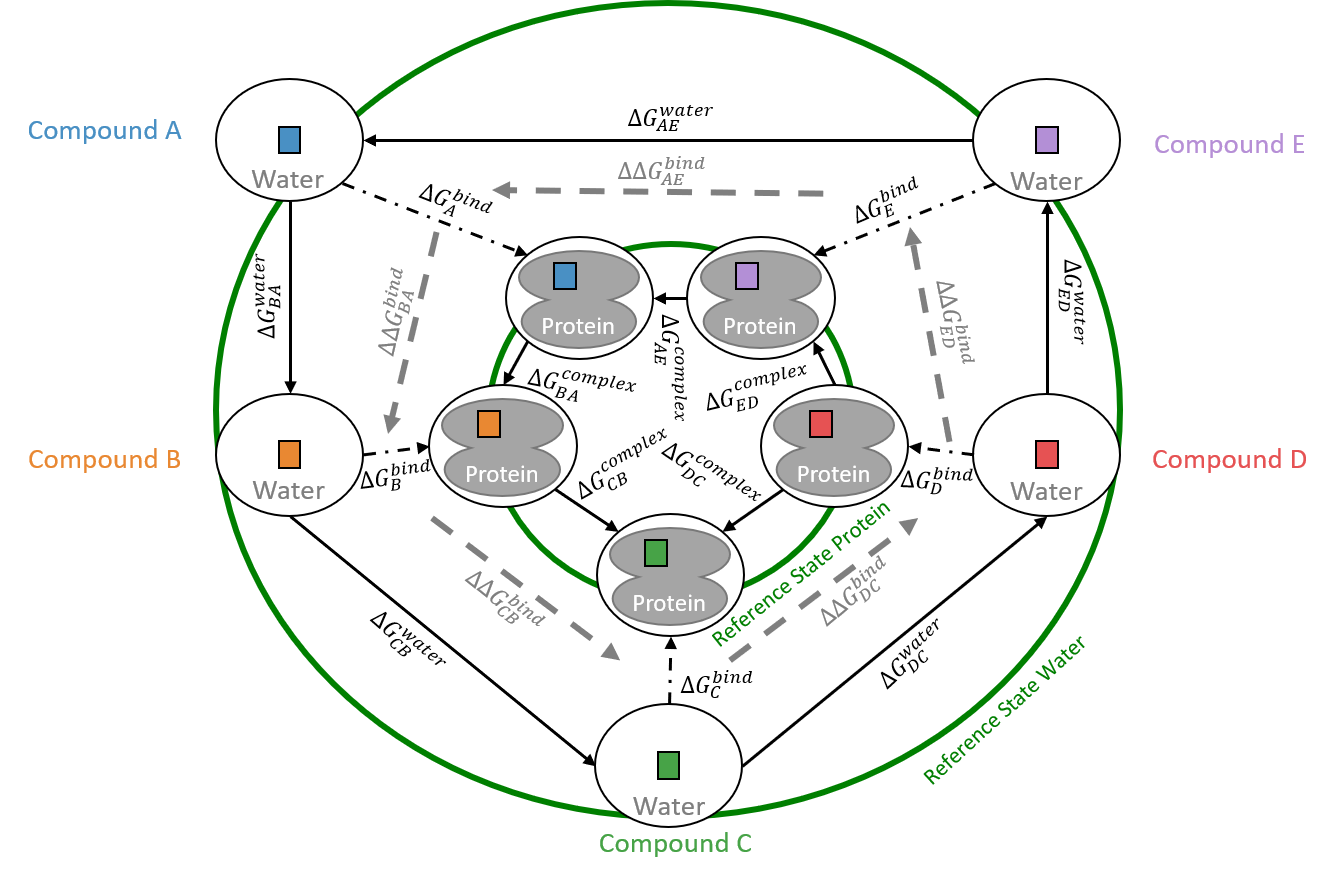
\includegraphics[width=\columnwidth]{fig/intro/State_graph.png}
    \caption{State graph to calculate relative binding free energies, where the nodes represent specific compounds $A$ - $E$ in a particular environment (water/protein). 
    The connecting (directed) edges describe the transformations from one end state to another. The dashed-dotted arrows denote the direct calculation of the (absolute) binding free energy of compound $A$ to the protein, $\Delta G_{A}^\text{bind}$, whereas solid arrows indicate alchemical transformations between compound $A$ to compound $B$ in a given environment. From the resulting $\Delta G_{BA}^\text{env}$, $\Delta \Delta G^\text{bind}_{BA}$ can be calculated and compared with the value obtained from the difference of the experimentally determined $\Delta G_{i}^\text{bind}$ (gray dashed arrows).
    In pathway-dependent methods, each edge between two end states is calculated separately. With (RE-)EDS, all end states in a given environment can be considered simultaneously in a single simulation of a reference state (green circles).}
    \label{fig: StateGraph}
\end{figure}

%The advantage of pathlessness
An attractive and more efficient alternative to path-dependent methods is to simulate a reference state, which includes all $N$ end states simultaneously, without the specification of pathways (green rings in Figure \ref{fig: StateGraph}). Such a reference state is provided by the EDS \cite{Christ2007, Christ2008, Christ2009, Riniker2011} method. The EDS reference state can be further tuned for optimal sampling with parameters. Note that cycle closure is guaranteed by definition in this approach.
%
In order to enhance sampling further, combinations of EDS with enhanced sampling methods were developed such as replica-exchange EDS (RE-EDS) \cite{Lee2014, Sidler2016, Sidler2017} and accelerated EDS \cite{Perthold2018, Perthold2020}.

%conclusion:
In this study, we present an improved automated workflow for RE-EDS simulations that was restructured into two phases. The first phase aims to automatically estimate method parameters that otherwise had to be provided by the user. The second phase automatically optimizes the estimates from the first phase to retrieve a robust parameter set. The final production phase calculates the relative binding free energies of multiple ligands from a single simulation per environment. 
The robustness and versatility of the RE-EDS workflow are demonstrated on a series of five inhibitors of human checkpoint kinase 1 (CHK1) \cite{Huang2012}.
These ligands were selected by Wang \textit{et al.} \cite{Wang2017} as a challenging benchmarking set for FEP calculations since the changes between these ligands exemplify different types of core-hopping transformations (i.e. ring size change, ring opening/closing, and ring extension). Special soft bond-stretching terms were developed to be able to handle these transformations \cite{Wang2017}. In contrast to many other methods, no such special soft bonds are required with RE-EDS as we can use a ``dual topology'' approach \cite{Riniker2011} in a straightforward manner. 
\FloatBarrier

%================================================================================
\section{Theory}
%================================================================================

\label{ch:3Theory}
\subsection{Enveloping Distribution Sampling (EDS)}
In EDS, free-energy differences between multiple end states are obtained by sampling a reference-state Hamiltonian, i.e. without the definition of specific alchemical paths \cite{Christ2007,Christ2008,Riniker2011}. 
Given $N$ end states, the potential energy function $V$ of the EDS reference state $R$ is defined as,
\begin{equation}
    V_R(\textbf{r}; s, \textbf{E}^R)= - \frac{1}{\beta s}\ln \left[ \sum^N_{i=1}{e^{-\beta s \left(V_i(\textbf{r})- E_i^R\right) }} \right] ,
    \label{EQ: Reference EDS}
\end{equation}
where $\beta = (k_\mathrm{B} T)^{-1}$ with $k_\mathrm{B}$ being the Boltzmann constant and $T$ the absolute temperature.
The smoothing parameter $s$ and the energy offsets $\textbf{E}^R$ were introduced to enable tuning of the reference state for optimal sampling of all end states \cite{Christ2007, Christ2008}.

%% $s$-parameter    
A smoothness parameter set to $s=1.0$ gives a reference potential-energy landscape that contains all the relevant minima of the end states. However, these might be separated by high barriers.
For $s < 1$, the energy barriers between different end states $V_i$ are smoothed in the reference potential $V_R$, increasing the transition rates between the different minima (Figure \ref{fig: EDS_potential_behaviour}A) \cite{Christ2008}. 
However, if $s$ is chosen too small, $V_R$ consists of a global unphysical minimum, which does not correspond to any of the end states. 
In the limit of $s\rightarrow 0$, all end states contribute equally to the potential-energy function of the reference state \cite{Koenig2020}, which can lead to unphysical deformations. The situation with a too small $s$ has been termed ``undersampling'' \cite{Riniker2011}.



%%Eoff
The energy offsets $\textbf{E}^R$ are used to ensure equal weighting of all end states $V_i$ in $V_R$ (Figure \ref{fig: EDS_potential_behaviour}B). 
Note that the optimal values of $s$ and $\textbf{E}^R$ are not independent of each other (as can be seen in Eq. (\ref{EQ: Reference EDS})) \cite{Christ2008}.
%
Different schemes have been proposed to determine optimal reference-state parameters \cite{Riniker2011, Christ2009, Hansen2012}, however, these are only applicable to systems with two end states.

\begin{figure}[h]
    \begin{center}
    \begin{subfigure}{0.44\columnwidth}
        \centering
        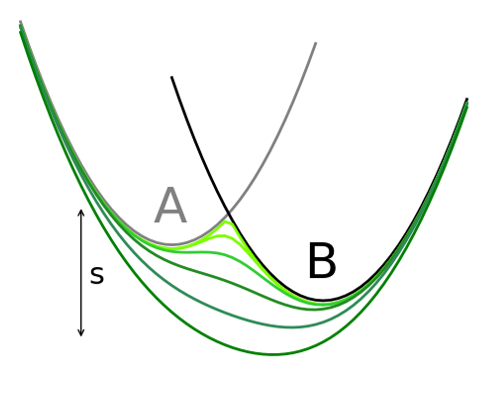
\includegraphics[width=\textwidth]{fig/intro/EDS_parmeters_s.png}
        \caption{Effect of $s$ on $V_R$}
        \label{fig: EDS_potential_behavioura}
    \end{subfigure}
    \begin{subfigure}{0.44\columnwidth}
        \centering
        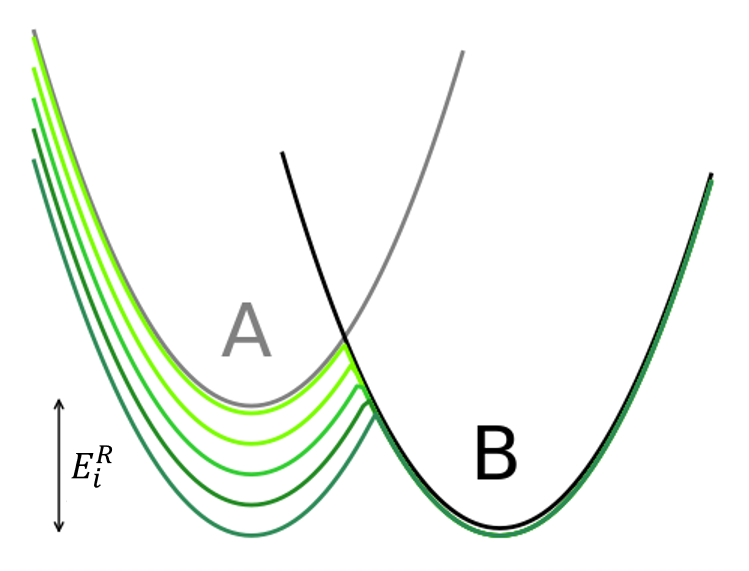
\includegraphics[width=\textwidth]{fig/intro/EDS_parmeters_Eoff.png}
        \caption{Effect of $E_i^R$ on $V_R$}
        \label{fig: EDS_potential_behaviourb}
    \end{subfigure}
    \end{center}
    \caption{Schematic illustration of the effect of the two types of EDS reference-state parameters. (\textbf{A}): The smoothing parameter $s$ decreases the barriers between the end states. If $s$ is too small, an ``undersampling'' situation occurs with a global unphysical minimum. (\textbf{B}): The energy offsets $\textbf{E}^R$ provide equal weighting to all end states in the EDS reference state.  The figure was generated with Ensembler\cite{Ries2021} (Chapter \ref{ch:feens}).}
    \label{fig: EDS_potential_behaviour}
\end{figure}

% laws of motion of R
The force on a particle $k$ in the EDS reference state is calculated as \cite{Christ2008},
\begin{equation}
    \textbf{f}_k(t)=-\frac{\partial V_R(\textbf{r}; s, \textbf{E}^R)}{\partial \textbf{r}_k} = \sum^N_{i=1}\frac{e^{-\beta s(V_i(\textbf{r}) -E_i^R)}}{\sum^N_{j=1}{e^{-\beta s (V_j(\textbf{r})-E_j^R)}}}  \left( -\frac{\partial V_i(\textbf{r})}{\partial \textbf{r}_k} \right) \,.
    \label{eq:laws_of_motion}
\end{equation}
%
For $s$ values close to one, the reference-state forces are dominated by the one end state, for which the current coordinates are most favourable, while the other end states give high energies and therefore contribute little (i.e. ``dummy states'').  
For small $s$ values (undersampling situation), all end states contribute effectively to the forces, resulting in the global unphysical minimum.

%% ddFE
The free-energy difference between two end states $A$ and $B$ can be calculated by employing the Zwanzig equation twice forming a path via the reference state~$R$ \cite{Zwanzig1954,Christ2007,Christ2008},

\begin{align} \nonumber
    \Delta G_{\text{BA}} &=  \Delta G_{\text{BR}} + \Delta G_{\text{RA}} \\ 
    &=-\frac{1}{\beta}\left(\ln \langle e^{-\beta (V_B-V_R)}\rangle_R - \ln \langle e^{-\beta (V_A-V_R )}\rangle_R\right) \\ 
    &= -\frac{1}{\beta} \ln \frac{\langle e^{-\beta (V_B-V_R)}\rangle_R}{\langle e^{-\beta (V_A-V_R)}\rangle_R}.
    \label{EQ: Free Energy calculation via reference state}
 \end{align}

%---------------------------
\FloatBarrier

\subsection{Replica-Exchange EDS (RE-EDS)}
The recently introduced RE-EDS method \cite{Sidler2016,Sidler2017} is a type of Hamiltonian replica exchange \cite{Hansmann1997,Sugita2000} with the smoothness parameter $s$ as the exchange dimension ($1 \geq s > 0$), which was inspired from constant pH simulations by Lee \textit{et al.} \cite{Lee2014,Lee2015}. The approach is shown schematically in Figure \ref{fig:RE-EDS_Scheme}.
RE-EDS does not require a single (optimal) $s$-value. Instead enhanced sampling is achieved by exchanging between the replicas with different smoothness levels. This simplifies the parameter choice problem and thus, the method can be applied to systems with more than two end states \cite{Sidler2016,Sidler2017}.

%Exchange criterium
For the pairwise exchanges between neighboring replicas $k$ and $l$, a Metropolis-Hastings criterion \cite{Hastings1970} is used \cite{Sidler2016,Sugita2000},
\begin{equation}
    \begin{split}
    p_{k,l} = min\bigg(1, \exp \Big[
                &-\beta \big((H_{R}(\textbf{r}_k; s_l)+H_{R}(\textbf{r}_l; s_k))\\
                &-(H_{R}(\textbf{r}_l; s_l)+H_{R}(\textbf{r}_k; s_k))\big)  \Big] \bigg) ,
    \end{split}
\end{equation}
where $H_{R_k}$ and $H_{R_l}$ are the reference-state Hamiltonians of the respective replicas, $\textbf{r}_k$ and $\textbf{r}_l$ are the current coordinates of the replicas.

Replicas are placed between $s=1.0$ and a lower bound of $s$, where the reference state is in undersampling. The replicas with low $s$ values facilitate the transitions between the low-energy regions of the  different end states. Especially for systems with slowly adapting environments (e.g. protein binding pockets), regions in $s$-space with very low acceptance probability can occur. Thus, to ensure sufficient exchanges between all pairs of replicas, a local variant of the round-trip time optimization algorithm \cite{Katzgraber2006, Nadler2008} was developed to optimally place the replicas in $s$-space \cite{Sidler2017}.
It was found that a single set of energy offsets can be used for all replicas \cite{Sidler2016}. However, it is important that these energy offsets are chosen well to avoid ``leakage'' effects, resulting in one or more end states not being properly sampled \cite{Sidler2016}.
The final free-energy differences are estimated from the replica at $s=1.0$, which represents the physical minima of the end states.

\begin{figure}[h]
    \centering
    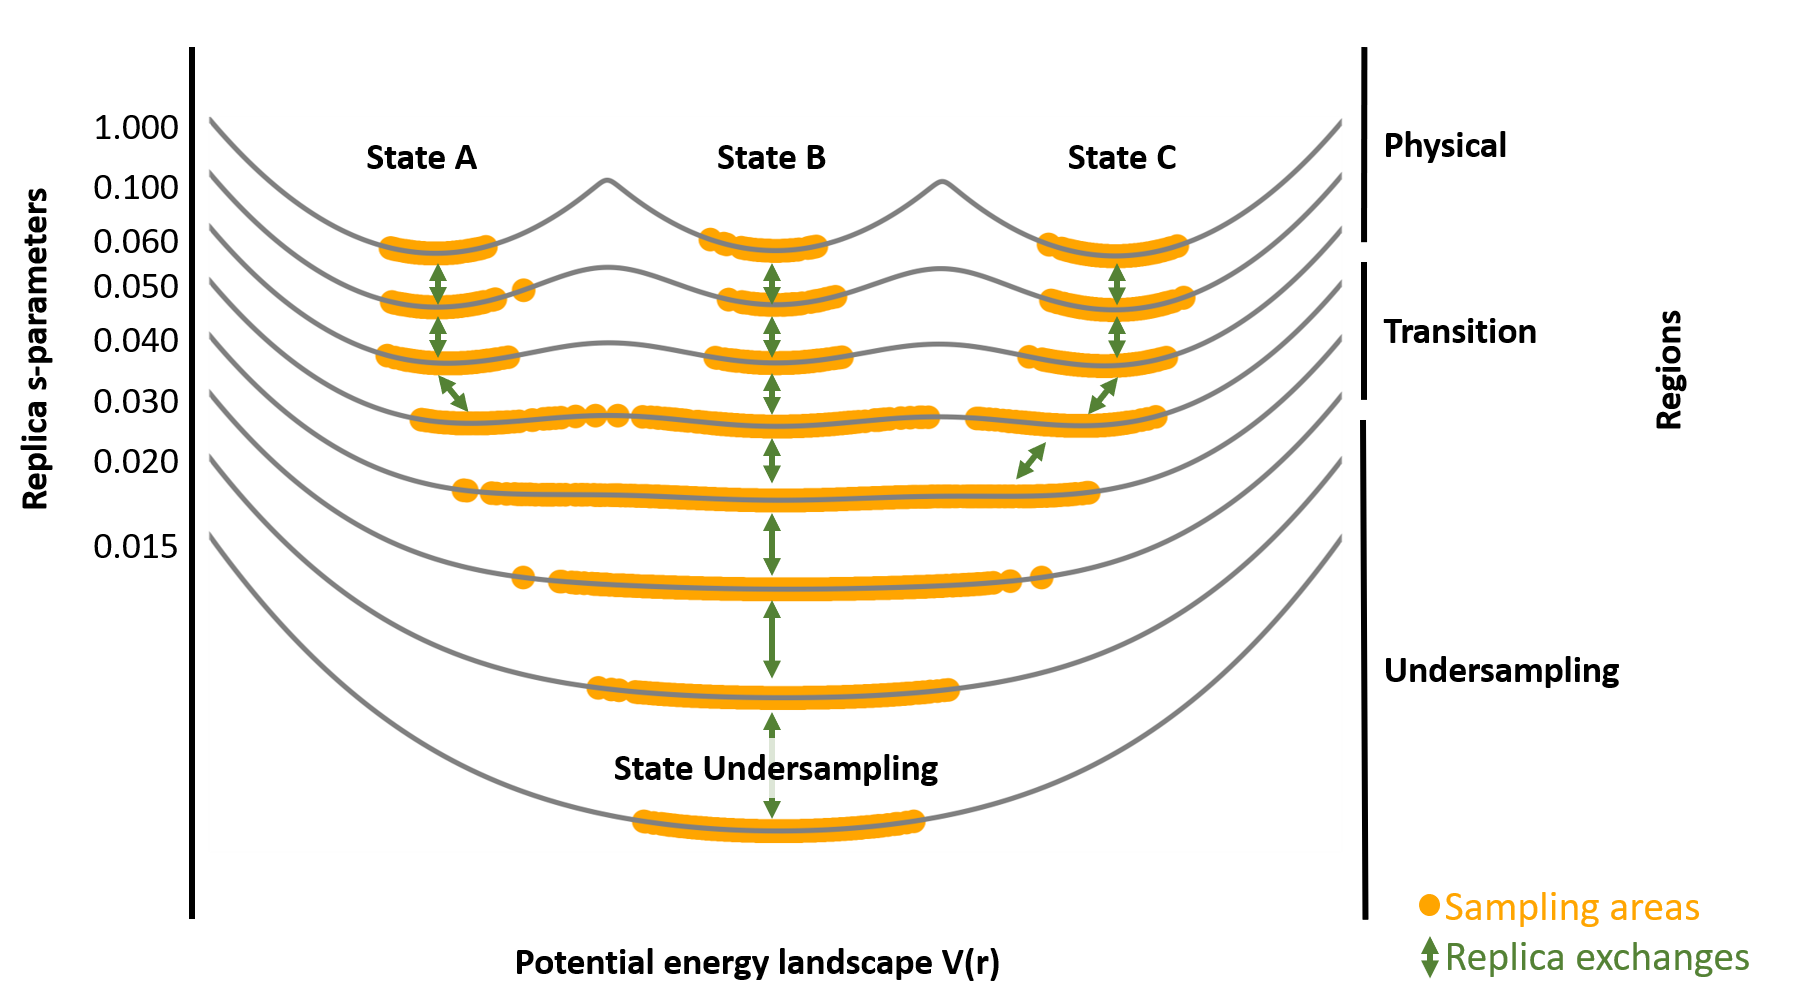
\includegraphics[width=\columnwidth]{fig/theory/Reeds_scheme_first.png}
    \caption{Schematic illustration of RE-EDS with three harmonic oscillators as end states ($A$, $B$, and $C$). Each replica differs by the $s$-parameter, generating reference states with a different degree of smoothness. Sampling of each replica is denoted with orange dots. Exchanges between the replicas are indicated with green arrows. The replica graph shows three regions: a ``physical'' region where $s$ is close to 1, a transition region, and the ``undersampling'' region when $s$ approaches zero. The figure was generated with Ensembler \cite{Ries2021}  (Chapter \ref{ch:feens}).}
    \label{fig:RE-EDS_Scheme}
\end{figure}

%---------------------------
\FloatBarrier

\subsection{Automatic Parameter Optimization}
To facilitate the determination of the energy offsets and $s$-parameter distribution, we have extended and further automatized the previous \cite{Sidler2017} RE-EDS workflow (Figure \ref{fig:Workflow}).
\begin{figure}[h!]
    \centering
    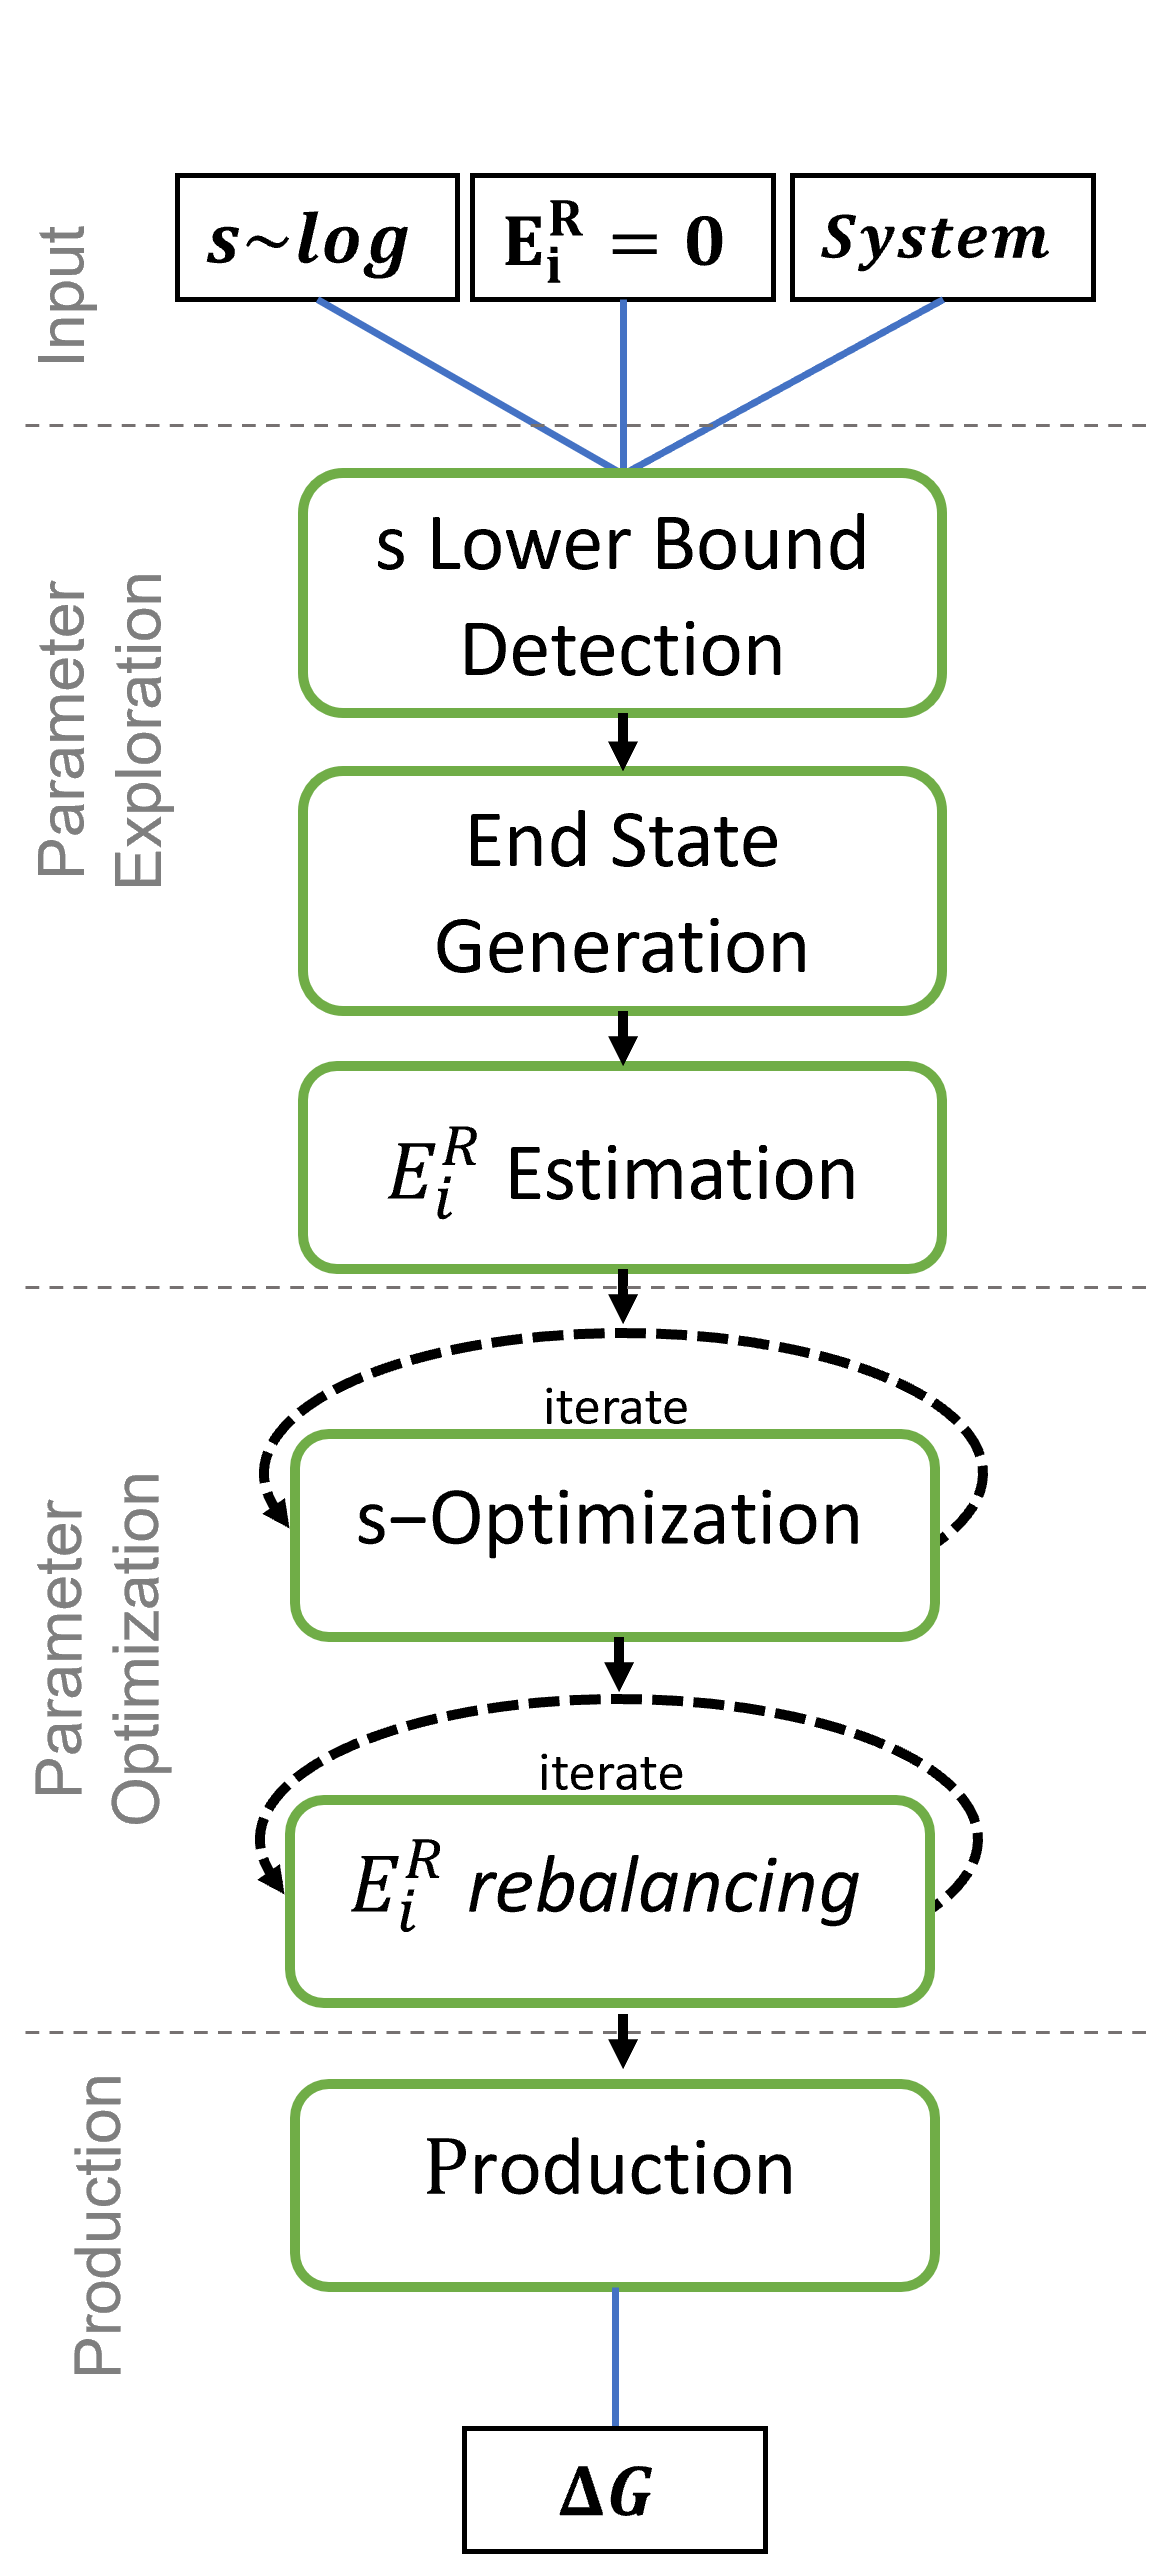
\includegraphics[width=0.5\columnwidth]{fig/theory/RE_EDS_Pipeline.png}
    \caption{The RE-EDS workflow can be split into four steps: (1) Input stage with energy offsets set to $E_i^R=0$ and a set of $s$-parameters logarithmically distributed between $1$ and $10^{-5}$; (2) Parameter exploration to determine the lower bound for $s$, to obtain equilibrated coordinates for each end state, and to estimate initial energy offsets with the PEOE scheme \cite{Sidler2016}; (3) Parameter optimization to improve the $s$-distribution with the N-LRTO algorithm \cite{Sidler2017} and the state sampling with energy offset rebalancing; (4) Production run and calculation of the free-energy differences.}
    \label{fig:Workflow}
\end{figure}

%
The initial input for a system with $N$ end states consists of a prepared EDS system (i.e. topology,  perturbation topology, initial coordinates, and distance restraints), a list of energy offsets of length $N$ with $E_i^R = 0; ~ \forall ~ i \in [1,...,N]$, and a list of $s$-parameters, which are logarithmically distributed in the range $s_i \in [1, 10^{-5}]$. Typically, we use 21 initial $s$ values. 

The parameter exploration consists of three substeps: (i) determining the lower bound for the $s$-distribution (newly introduced), (ii) obtaining optimized coordinates within the EDS set-up for each end state (newly introduced), and (iii) estimation of an initial set of energy offsets (as done previously in Ref.~\citenum{Sidler2016}).

%%1. initial parameter search
To enable sampling of all end states at $s=1.0$, some replicas have to be in undersampling to facilitate transitions. However, for efficiency reasons (and numerical stability) the number of replicas $M$ in undersampling should be small and the lowest $s$-value should be as high as possible. From a short simulation with the initial $s$-distribution between $[1, 10^{-5}]$, the highest smoothing parameter $s_{M_\mathrm{us}}$ at which undersampling still occurs is determined and used in the following as a lower bound for the $s$-distribution. The $s$-distribution for the next step is then defined by logarithmically distributed replicas between $s=1.0$ and the automatically determined lower bound.

%%%state optimization
Optimized coordinates for each end state in the EDS setup can be automatically obtained by short parallel simulations, where one end state in turn is favoured by setting an arbitrarily large energy offset for this state. 
The optimized coordinates allow the user to start RE-EDS simulations from different end states and are needed for the subsequent parameter optimization. 

 %%% estimate EOFFs:
In the last substep, $E_{\text{i}}^{\text{R}}$ estimation, the previously developed parallel energy offset estimation (PEOE) \cite{Sidler2016} scheme is used to estimate the initial set of energy offsets. This is done based on a short simulation with the initial parameters. For each replica $k$ in the undersampling region, the energy offsets are extracted using \cite{Sidler2016},
\begin{equation}
    E_{i}^{R}(new)=-\frac{1}{\beta}\ln \Big < e^{-\beta \big(V_i(\textbf{r})-V_R(\textbf{r}; s_{k},\textbf{E}^{R}(old))\big)}\Big>_{R(s_{k},\textbf{E}^{R}(old))} .
    \label{eq: EoffEstimator}
\end{equation}
The energy offsets that were extracted in parallel for the $k$ replicas are subsequently averaged and used as initial set of energy offsets. These energy offsets should provide a first solution that is close to the optimal choice of energy offsets, which leads to an optimal state sampling of all end states in the RE-EDS simulation. As the initial energy offsets are obtained from the replicas in undersampling, they may not be exactly optimal and require fine-tuning in the next phase. 


%%2. optimization of parameters
In the second step of the RE-EDS workflow, first the $s$-distribution is optimized and subsequently the energy offsets are fine tuned.
%
%%% s-Optimization:
The $s$-distribution is improved by minimizing the round-trip time $\tau$ and increasing the number of round-trips, using the multistate local round-trip time optimization (N-LRTO) algorithm \cite{Sidler2017}. The optimization is performed in an iterative manner with short simulations.
This step is required as exchange bottlenecks between two replicas might occur leading to a very slow round trip time or to no round trips at all. 
In the N-LRTO algorithm, new replicas are inserted in each iteration by linear interpolation in the $s$-regions with exchange bottlenecks, while the replica positions of the previous iteration are retained. Adding replicas theoretically increases the round-trip time because of a longer path between the top and bottom replicas. However, the addition of intermediate replicas also increases the exchange probability between neighboring replicas, thus reducing the round-trip time. With the optimization algorithm, we aim to determine the balance between the length of the replica path and the likelihood of exchange between replicas for minimal round-trip time. The exchange bottlenecks are identified for each end state separately (i.e. multistate). The number of replicas added can be chosen by the user. The iteration is stopped when the average round-trip time $\overline{\tau}$ converges. 
The N-LRTO variant is needed for systems for which severe bottlenecks are observed with the initial logarithmic $s$-distribution (e.g. protein binding pockets). For systems with smaller perturbations, the global multistate variant (N-GRTO) \cite{Sidler2017} can be more efficient as this algorithm re-distributes the replicas in $s$-space according to the exchange statistics. %In very severe cases, this can lead to an oscillating behavior, as one bottleneck is fixed, but another appears due to an imbalance of replica shifting.
%
In this study, we started with the same number of replicas as used for the PEOE scheme above and added four replica positions per iteration in the N-LRTO algorithm.

%%%% Eoff Rebalancing:
After optimizing the number of round trips and $\tau$, the distribution of the state sampling is improved. To reach the ideal situation that each end state is sampled to an equal amount, the initial energy offsets need to be fine tuned, while keeping the round trips approximately constant. For this, we introduce here the energy offset rebalancing scheme.
To avoid overshooting, a correction factor is calculated and applied iteratively,
\begin{equation}
    \Delta E^{corr}_i = - \frac{1}{\beta} \ln \left( \frac{f_i^{\text{mc}}+c}{f^{\text{mc,ideal}}_{i}+c} \right),
    \label{eq: EoffRebalancing}
\end{equation}
where $f_i^{\text{mc}}$ is the current sampling fraction (or estimated probability) of an end state contributing to $V_R $, and $f^{\text{mc,ideal}}$ is the ideal sampling fraction (see Section \ref{metrics}). 
%
To make the approach more robust, a pseudo count $c$ is introduced to avoid singularities with zero sampling, which is defined as,
\begin{equation}
    c = \frac{f^{\text{mc,ideal}}}{x},
    \label{eq: EoffRebalancingPseudoCount}
\end{equation}
with the intensity factor $x$.
The default of the pseudo count was chosen to result in a maximal correction of $\Delta E^{corr}_i=8.43$~kJ/mol, corresponding to a minimum 30-fold reduced sampling compared to the expected optimal sampling.

%%% 3. production run
After optimizing the RE-EDS parameters, the production run is performed for a chosen length. 
The free-energy differences are subsequently calculated using the replica at $s=1.0$ with Eq.~(\ref{EQ: Free Energy calculation via reference state}).

\subsubsection{Starting State Mixing}
The sampling in RE-EDS simulations can be further improved by using starting coordinates for the replicas corresponding to the different end states (i.e. replica 1 starts in a low-energy configuration for end state 1, replica 2 in a low-energy configuration for end state 2, etc.). This technical approach is called ``starting state mixing'' (SSM) in the following and is also used for Hamiltonian replica-exchange TI calculations (see e.g. \citenum{Graf2016, Hahn2020}). The optimized coordinates obtained in the parameter exploration step can be used for SSM. We compare RE-EDS simulations with SSM and with a single set of starting coordinates (abbreviated as 1SS).  

\subsubsection{Analysis}
\label{metrics}
Three types of metrics were used to quantify the sampling in RE-EDS simulations. The first metric determines for each end state $i$ the sampling fraction where it is maximally contributing to the reference state, i.e. $f_i^{\text{mc}}$. A maximally contributing state is defined as the end state with the lowest potential energy minus its energy offset in a frame. As can be seen in  Eq.~\eqref{eq:laws_of_motion}, maximally contributing end states have the largest impact on the reference-state sampling at a given time point.

%
Optimal sampling in a RE-EDS system is achieved when all end states are sampled as maximally contributing states to an equal extent at $s=1.0$, i.e. 
\begin{equation}
f_{i}^{\text{mc,ideal}} = \frac{1}{N} ~, \forall ~ i~\in~ \{1, ..., N\}
\label{eq: optimalDominationSamplingDist}
\end{equation}

The second metric is the estimated sampling fraction of ``physical occurrence'' of an end state $i$, i.e. $f_i^{\text{occur}}$. As a result of phase-space overlap with the current maximal contributing end state, other end states in the EDS system might be sampled simultaneously. An end state is counted as ``occurred'' when its potential energy is below the threshold $V_i \leq T_{i}^{\text{phys}}$ at a time point $t$. 
These thresholds are estimated during the second substep of the parameter exploration phase. If end states show no phase-space overlap, $f_i^{\text{occur}}$ will be (nearly) the same as $f_i^{\text{mc}}$. 

Undersampling is detected with a third metric using the thresholds $T_{i}^{\text{us}}$. These thresholds are determined in the first substep of the parameter exploration phase from the simulation with the lowest $s$-value. If all end states have a potential energy below their respective $V_i - E^R_i \leq T_{i}^{\text{us}}$, the current frame is characterized as undersampling. \cite{Sidler2016} 

\FloatBarrier

%================================================================================
\section{Computational Details}
%================================================================================


\section{Toy model Comparisons}
To evaluate the introduced greedy approach, its performance was tested on randomly generated toy models. The models contained 12 to 30 particles that were randomly distributed in space. The particles were randomly assigned to two entities, representing two molecules. A selection of four restraints was simulated with no preprocessing filtering steps. Different algorithmic approaches were applied in the simulated selections: the introduced greedy approach, a 100 times repeated random selection, and two brute force approaches were used. One brute force approach maximized the distance between the selected restraints, and the other brute force approach maximized the CHV around the selected restraints like it is done for multistate system chaining. Each number of particles was sampled 20 times to give an insight into the uncertainty estimate of the particle placement. The scripts for this approach can be found in the example folder of our repository.

\subsection{Systems}
The systems for which the relative hydration free energies were calculated are selected sub-sets of the ATB Solvation Free Energy Database \cite{Martin2018}.

The solvation free energy calculations with the pairwise TI were carried out on a subset of $16$ molecules leading to 15 relative hydration free energies. The selected molecules represent transformations such as R-group changes and ring size changes, but also scaffold hopping transformations.

\begin{figure}[h]
    \centering
    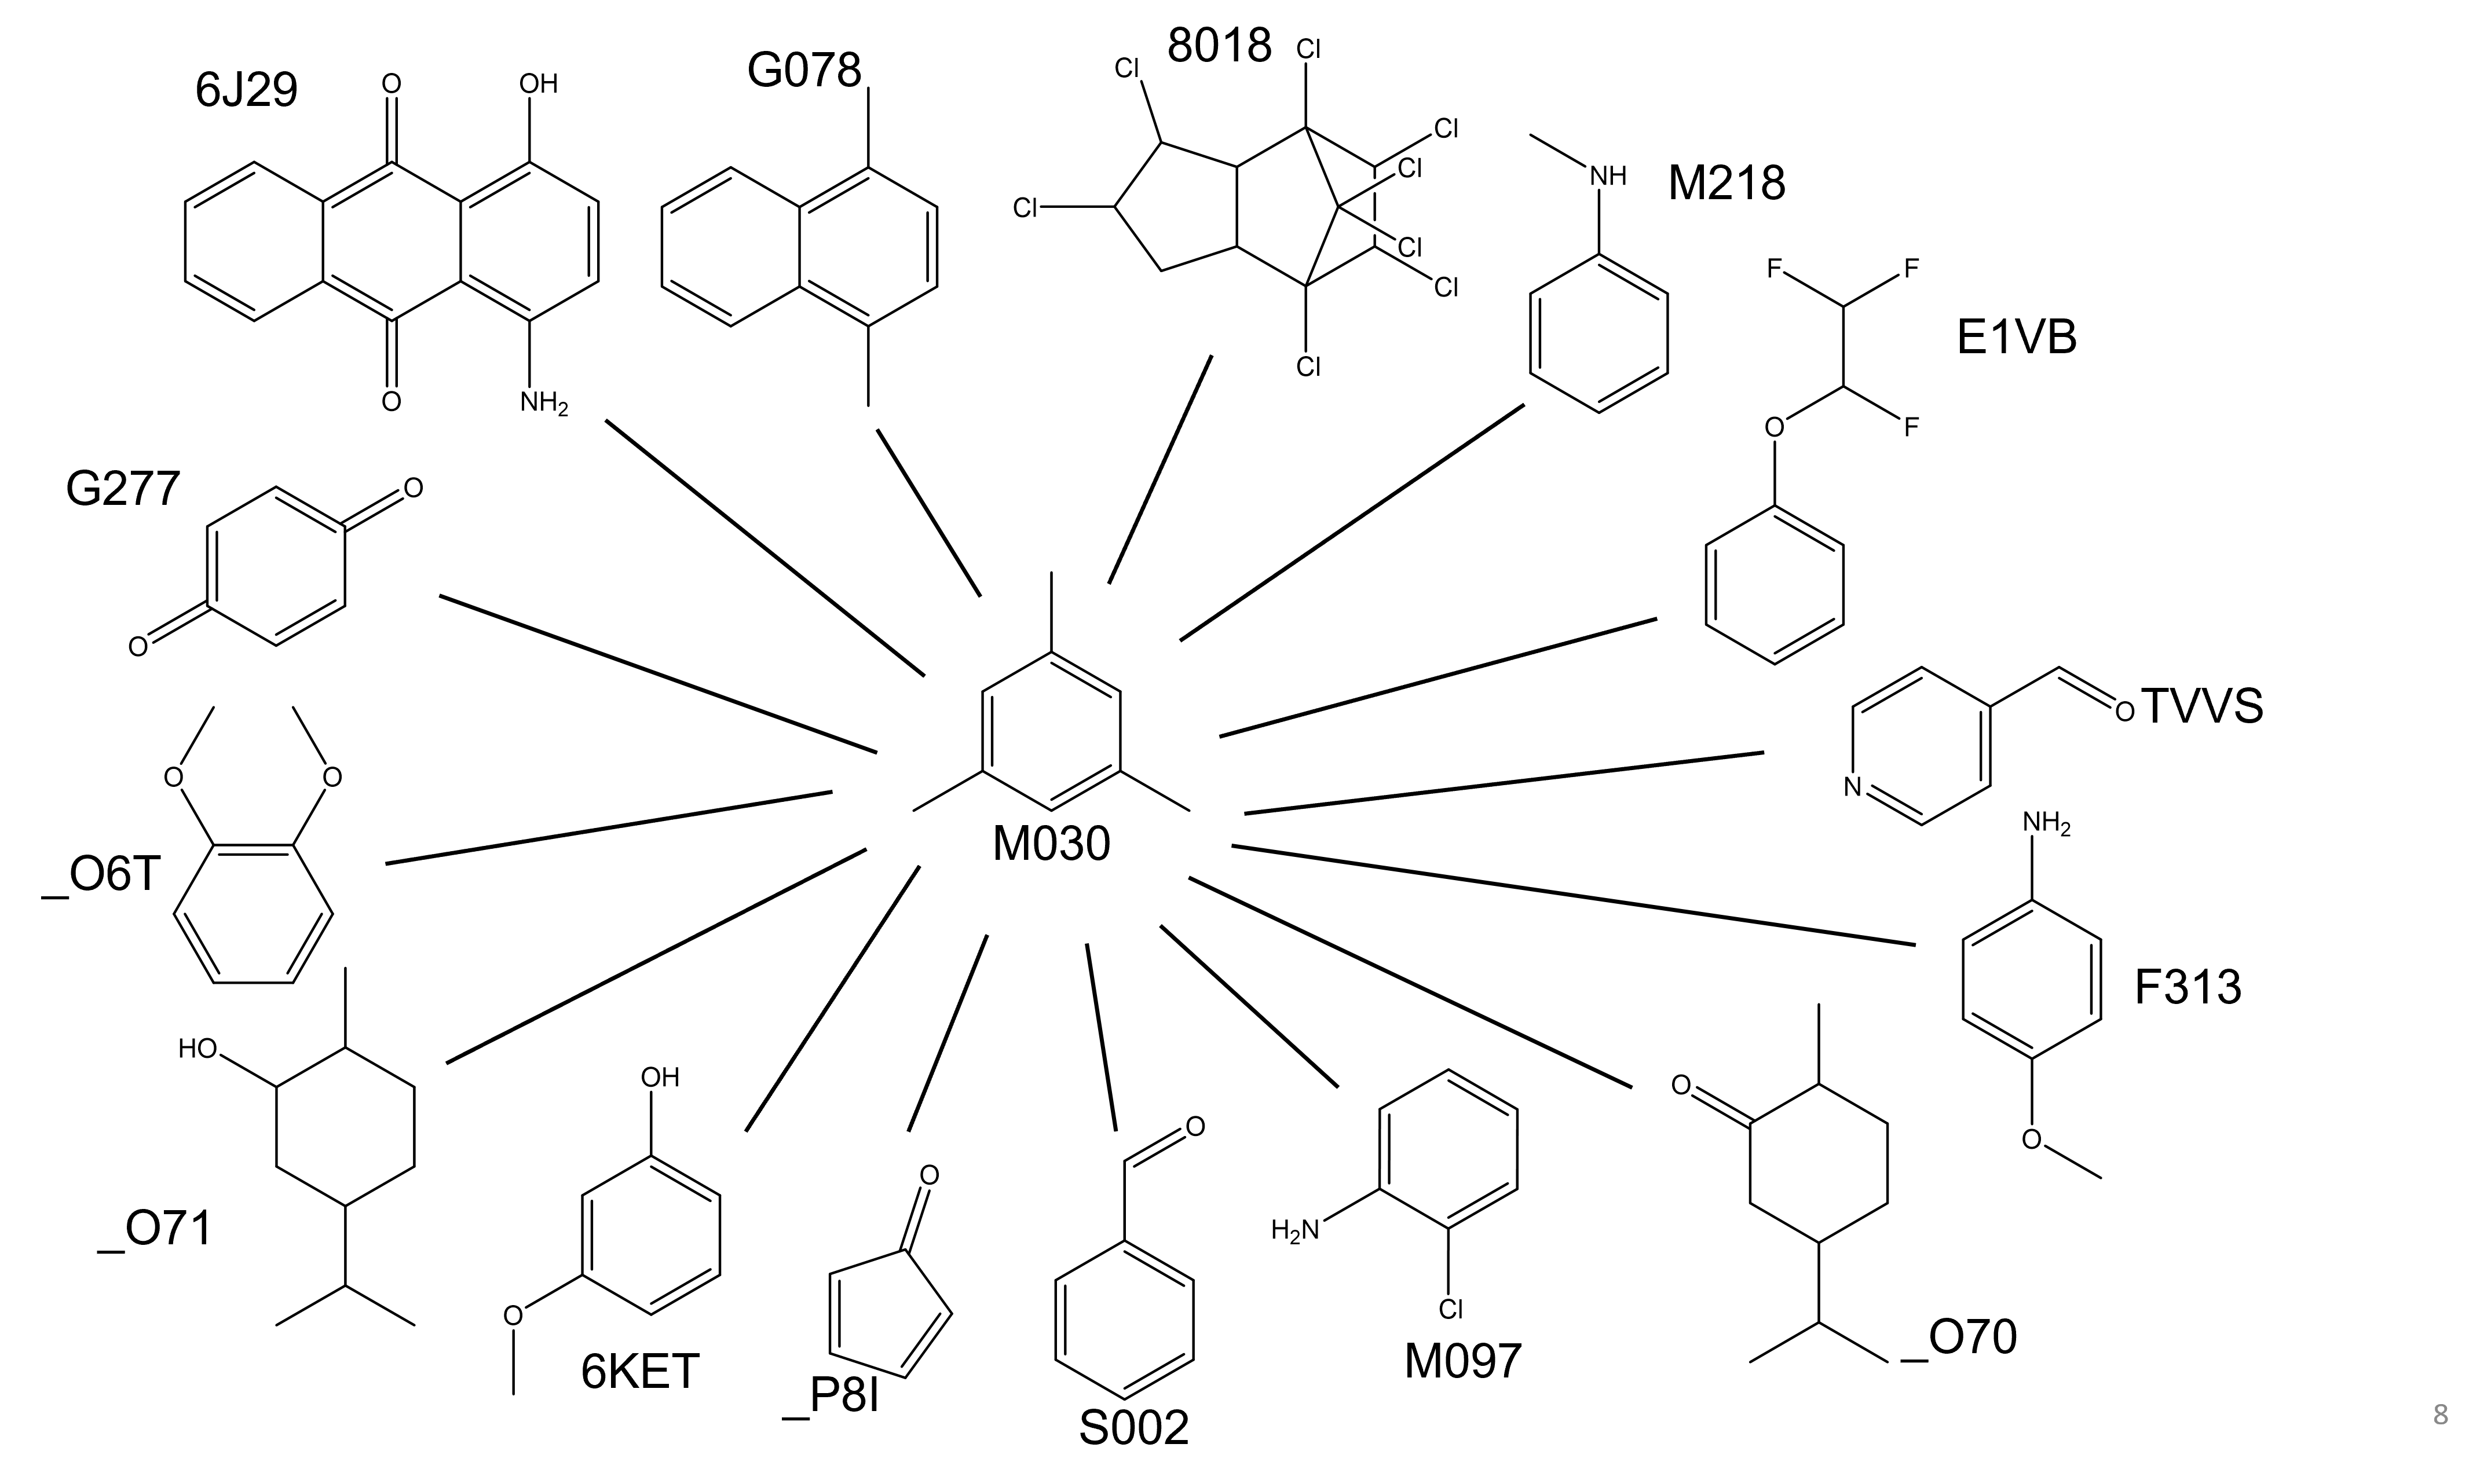
\includegraphics[width=\textwidth]{fig/methods/StateGraph_TI_2D.png}
    \caption{TI-Graph. In order to evaluate the restraints generated by RestraintMaker, a set of 16 molecules was chosen from the ATB Database.\cite{Martin2018} The set was chosen so it contained both relatively similar molecules with identical cores, as well as more difficult transformations such as scaffold hopping. The RestraintMaker was used to generate pairwise distance restraints between molecule M030 and the other molecules of the set. The relative hydration free energies were then calculated using TI with a linked dual topology approach with the generated distance restraints .}
    \label{fig: Pairwise_TI_M030_Graph}
\end{figure}

To apply our approach to multistate systems, two sub-sets of molecules were generated from the set of molecules selected for the pairwise TI simulations. The first subset A contains six molecules with the same core and transformations like R-group changes.

The second subset B for the multistate simulations increases the number of states and consists of 10 molecules. In this set, the complexity of the transformations is increased by a ring size change and a ring flexibility change.

\begin{figure}[h]
    \centering
    \begin{subfigure}{0.40\columnwidth}
        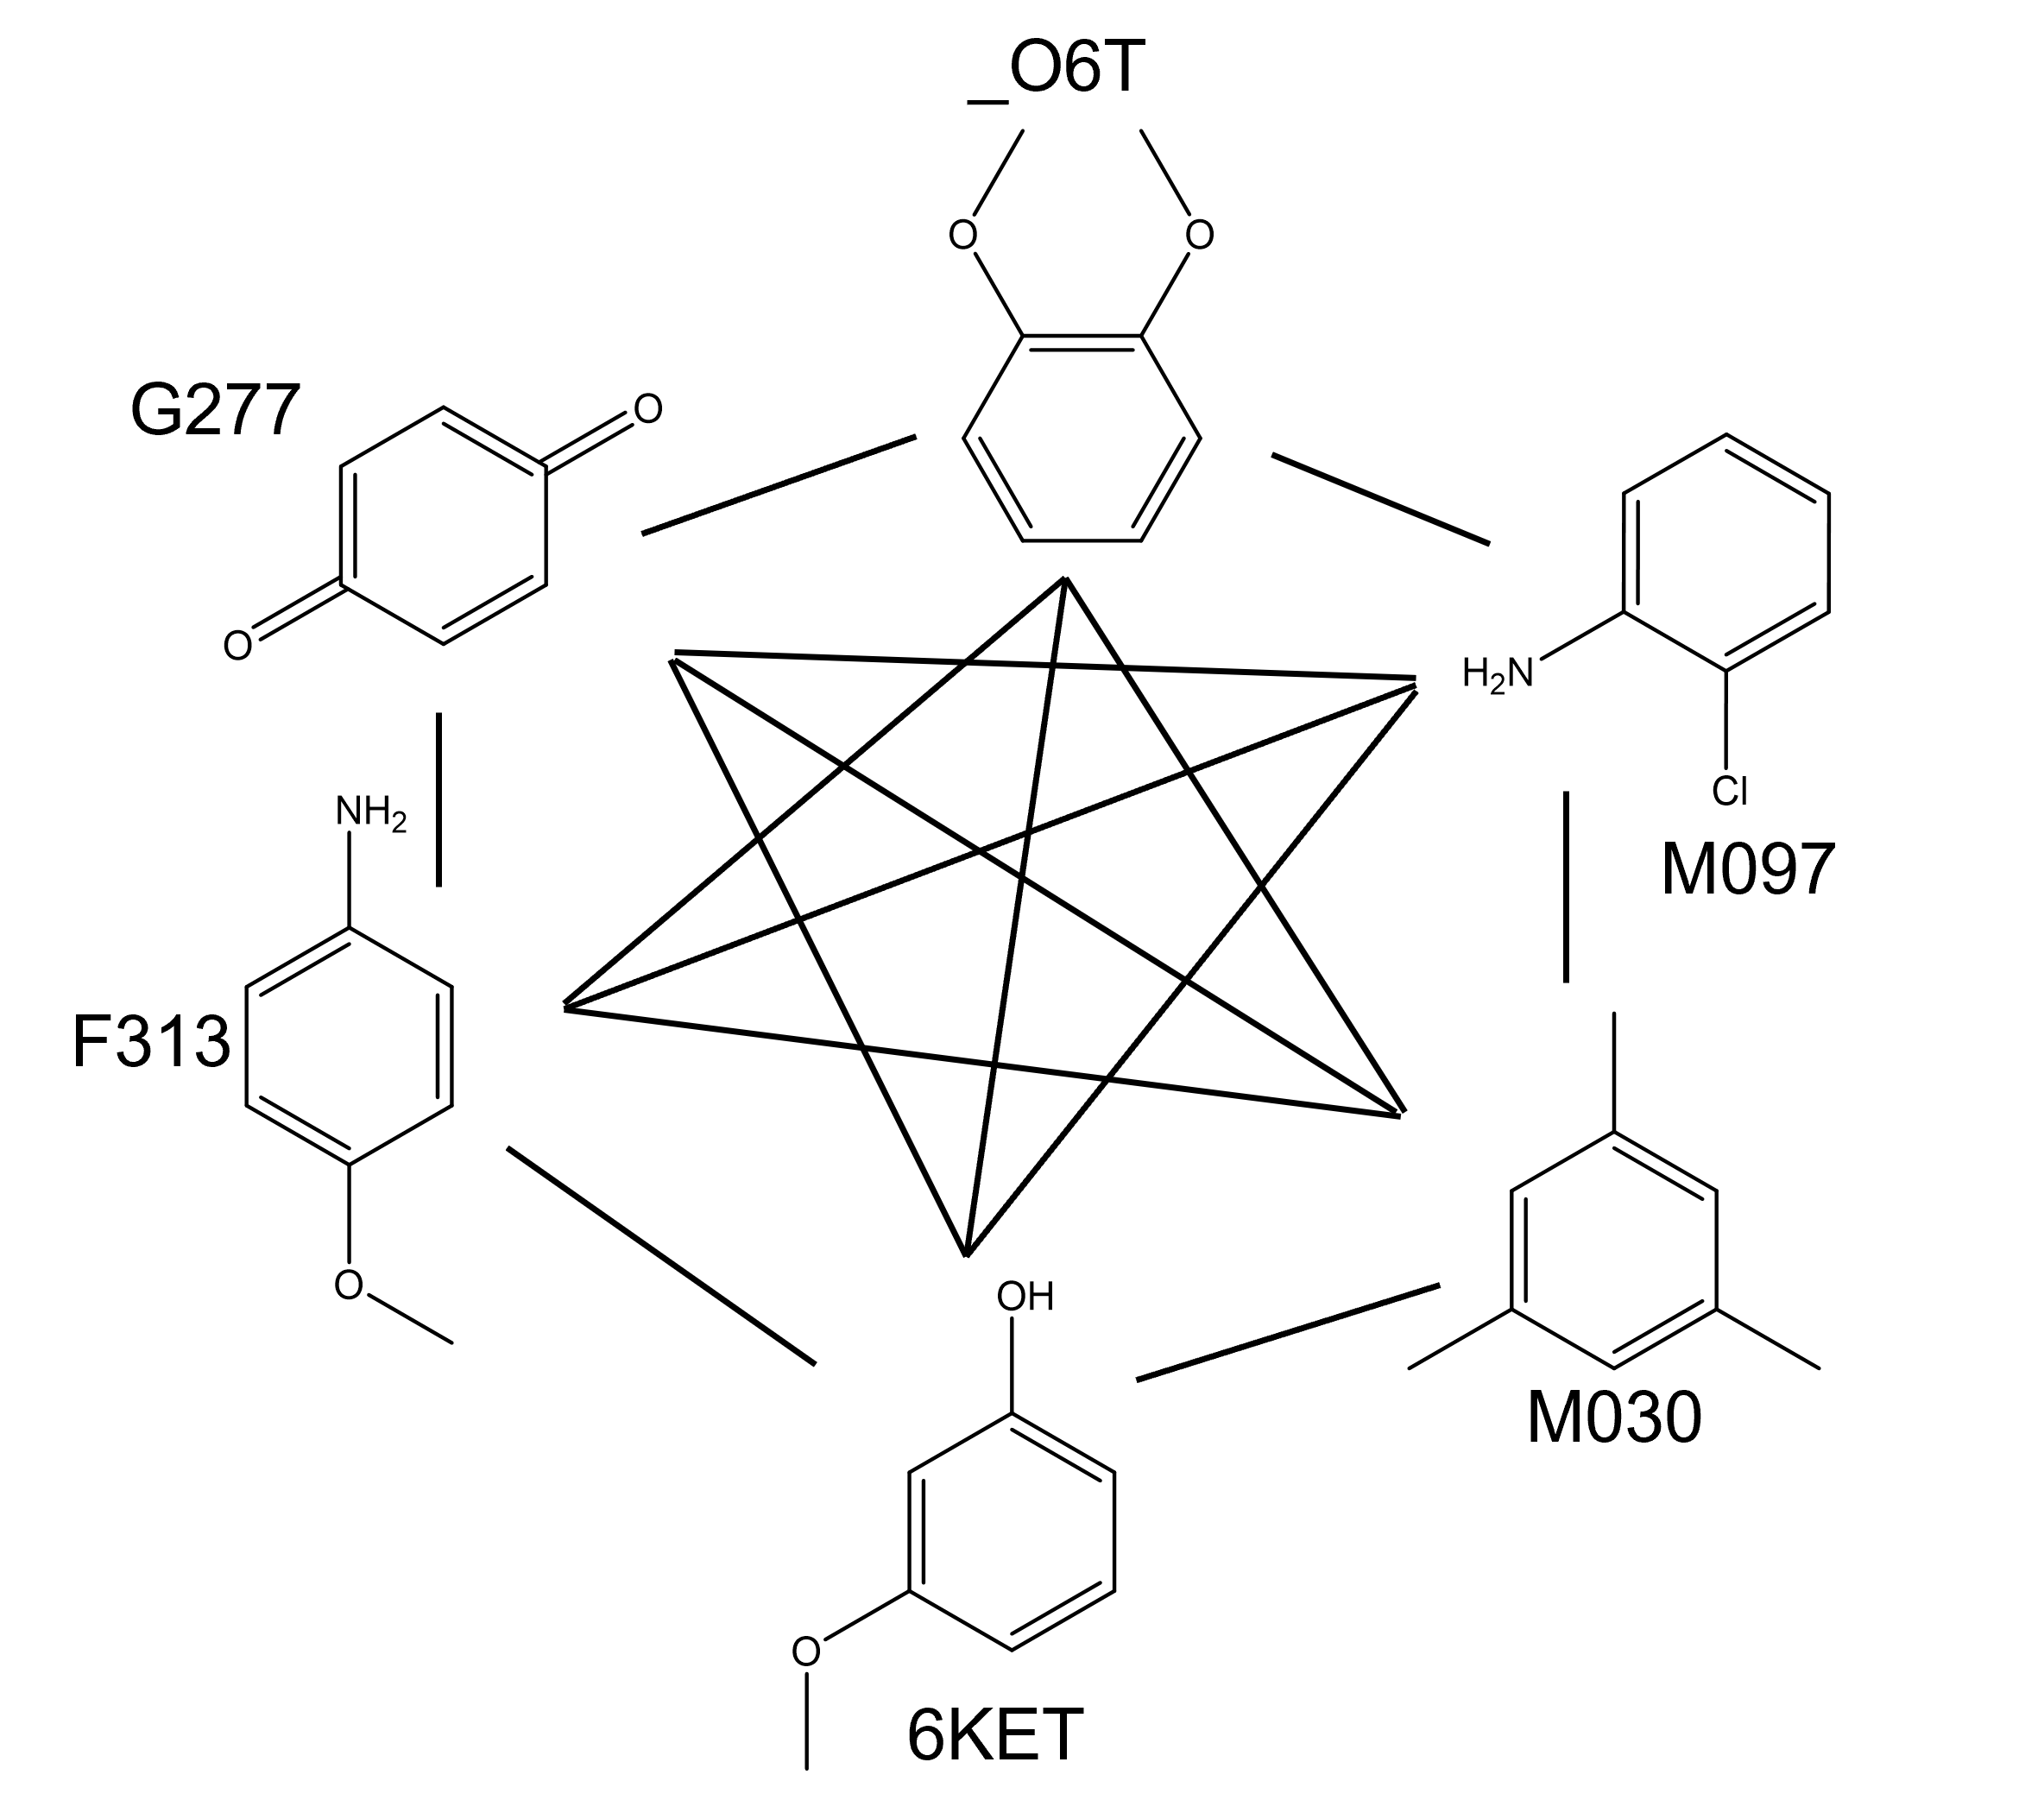
\includegraphics[width=\textwidth]{fig/methods/StateGraph_Multistate_easy6_2D.png}
        \caption{}
        \label{fig: multistate_6LigandsGraph}
    \end{subfigure}
    \begin{subfigure}{0.55\columnwidth}
        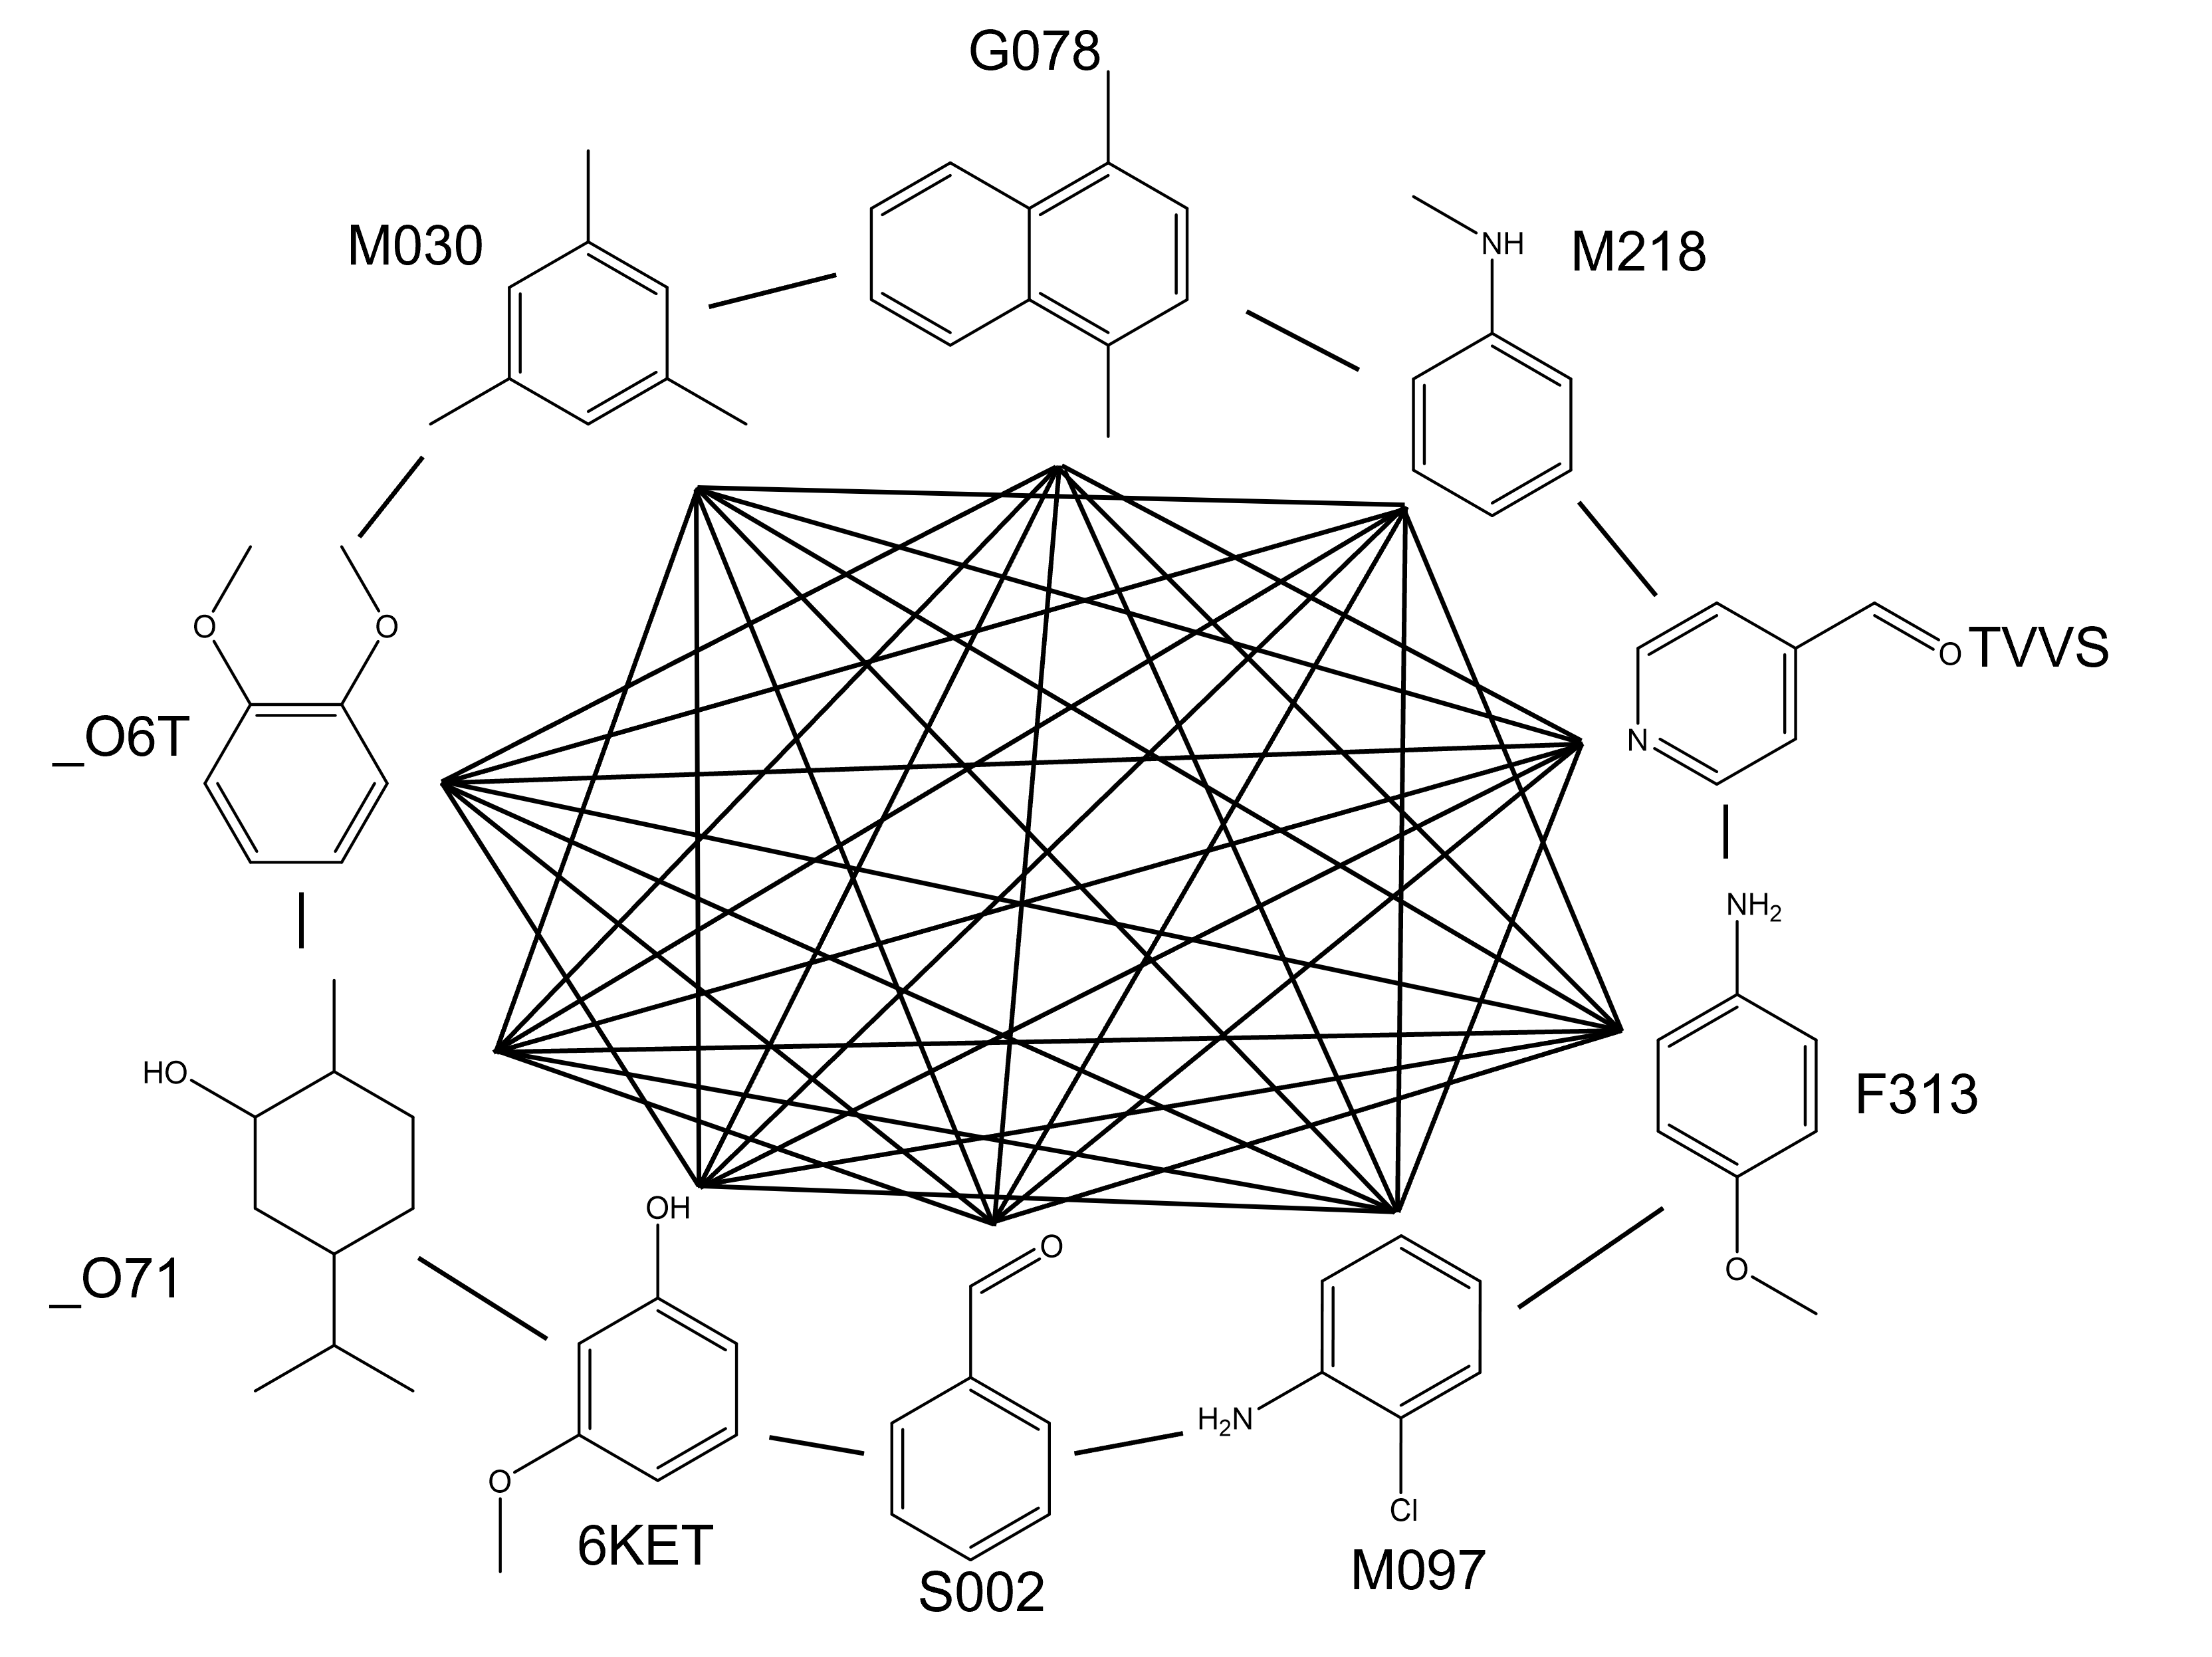
\includegraphics[width=\textwidth]{fig/methods/10state_flat_graph_2D.png}
        \caption{}
        \label{fig: multistate_10LigandsGraph}.
    \end{subfigure}
    \caption{Overview of the multistate systems. Two subsets were formed from the chosen molecules in Fig. \ref{fig: Pairwise_TI_M030_Graph} and all the possible transformation paths are indicated. \ref{fig: multistate_6LigandsGraph} Set A consists of six molecules, that contain mainly R-group and polarity transformations. \ref{fig: multistate_10LigandsGraph} Set B consists of 10 molecules that add to the transformations of set A ring flexibility changes}
    \label{fig: Subsets}
\end{figure}

The sets of molecules are depicted in Figures \ref{fig: Pairwise_TI_M030_Graph}, \ref{fig: multistate_6LigandsGraph}, and \ref{fig: multistate_10LigandsGraph}, respectively.

\subsection{Simulation Details}
The simulations were carried out using the molecular dynamics package GROMOS version 1.5.0 (freely available on \textit{http://www.gromos.net}),
the python RE-EDS pipeline package (\textit{https://github.com/rinikerlab/reeds}) 
and PyGromosTools (\textit{https://github.com/rinikerlab/PyGromosTools}). \cite{Schmid2012, Ries2021, Lehner2021} 

In order to compare the simulated results to the results reported in the ATB database, the same simulation setup was used. The topologies were taken from the ATB database. All simulations in water were carried out using the single-point charge (SPC) water model.\cite{Berendsen1981}. A single cutoff radius of $1.2$~nm was used for the calculation of the non-bonded interactions. The integration time step was set to $2$~fs and the pairlist was updated every five steps. Long-range nonbonded interactions were calculated using a reaction field correction with $\varepsilon_{rf}=1$ for the simulations in vacuum and $\varepsilon_{rf}=61$ for the simulations in water.\cite{tironi1995} The force constant for the distance restraints was set to $5000$ kJ$/($mol$\cdot$nm$)$.

\subsubsection{TI}
The thermodynamic integration was prepared by a short energy minimization with maximally 30000 steps and minimally $2000$ steps, converging if the potential energy is not changing anymore for larger values then $0.1~kJ$ . Next the TI was carried out with $21$ evenly spaced $\lambda$-windows between $1$ and $0$, both for water and vaccum environment. Each window was equilibrated for $1~$ns and afterwards a production run of $5~$ns was carried out. The free energies were calculated using the simpson integration of SciPy.\cite{Virtanen2020}

\subsubsection{RE-EDS}
The topologies for the RE-EDS calculations were prepared using PyGromosTools.\cite{Lehner2021} The simulations were carried out using the RE-EDS pipeline of Ries et al.\cite{Ries2021}.

For set A, six EDS simulations of $2$~ns were carried out in vacuum/water to generate optimized state configurations. 21 EDS simulations with s-values distributed logarithmically between $1$ and $10^{-5}$ were run for $200$~ps to determine the lowest s-value for the RE-EDS simulations such that undersampling was observed. For the simulations in vacuum, the lowest s-value was determined to be $0.00316$. For the simulations in water, the lowest s-value was determined to be 0.001. Next, the energy offsets were estimated from $800$~ps RE-EDS simulations. For the vacuum simulations, $12$ replicas were used and for the water simulations, $14$ replicas were used. In vacuum, one s-optimization run of $500$~ps was enough to ensure that roundtrips occurred in all replicas and all states were sampled well. 4 replicas were added. In water, three s-optimization runs of $500$~ps, $1000$~ps and $1500$~ps, respectively, were used to achieve roundtrips in all replicas. After each s-optimization run, five replicas were added. Additionally, for the simulation in water, the energy offsets were rebalanced during three $500$~ps RE-EDS energy offset rebalancing runs to ensure that all states were sampled equally. This was not necessary for the vacuum simulations, as all states were already sampled well after the s-optimization. Finally, a $500$~ps RE-EDS simulation was used to calculate the free energy differences in vacuum. In water, a $1$~ns RE-EDS simulation was used to calculate the free energy differences.

For set B, ten EDS simulations of $2$~ns were used in vacuum/water to generate optimized configurations for the ten molecules. As for set A, $21$ $200$~ps EDS simulations were carried out with logarithmically distributed s-values between $1$ and $10^{-5}$. The lowest s-value for the vacuum simulations was determined to be $0.00178$, and for the simulations in water $0.001$. For the energy offset estimation a $800$~ps RE-EDS simulation was used. For the simulation in water, $18$ replicas were used and for the simulation in vacuum, $17$ replicas were used. As for set A, only one s-optimization RE-EDS simulation of $500$~ps was needed in vacuum. Again, $4$ replicas were added. However, for the simulation in water, five s-optimzation runs of $500$~ps, $1000$~ps, $1500$~ps, $1500$~ps and $1500$~ps, respectively, were needed to ensure sufficient roundtrips in all replicas. At each s-optimization iteration, five replicas were added. While the energy offset rebalancing step could again be skipped for the simulation in vacuum, the energy offsets for the water simulation were rebalanced in 5 RE-EDS runs of $500$~ps. In order to determine the free energy differences in vacuum, a $1$~ns RE-EDS simulation was carried out. A $5$~ns RE-EDS production run was used to calculate the free energy differences in water.

More details on the RE-EDS pipeline and its substeps can be found in the work of Ries et al.\cite{Ries2021}

\subsection{Analysis}
The analysis of the simulations was done using \textit{GROMOS++} \cite{eichenberger2011} and PyGromosTools \cite{Lehner2021}. Further, the  following python packages were used for the statistical analysis and plotting: pandas \cite{Mckinney2010}, Matplotlib \cite{Hunter2007}, NumPy \cite{VanDerWalt2011}, SciPy \cite{Virtanen2020}, mpmath \cite{Johansson2013} and Jupyter notebooks.\cite{Kluyver2016}.

%================================================================================
\section{Results and Discussion}
%================================================================================

The chosen model system of five inhibitors of CHK1 kinase exemplifies different core-hopping transformations (i.e. ring size change, ring opening/closing, ring extension) and R-group modifications \cite{Wang2017}, increasing the complexity compared to the systems previously studied with RE-EDS. Furthermore, the performance can be directly compared to the results obtained with FEP+ and OPLS3 in Ref.~\cite{Wang2017} as well as with QligFEP results in Ref.~\cite{Jespers2019}.

\subsubsection{Parameter Exploration and Parameter Optimization}
The RE-EDS workflow was started by estimating the lower bound for the $s$-distribution. Using the above mentioned undersampling criterion (see Methods section), a lower bound of $s=0.01$ was determined for the protein-ligands complex and $s=0.0056$ for the ligands in water. 

%State Optimizations
Optimized coordinates were obtained for all five ligands, as verified by comparing the potential-energy distribution from the EDS simulation with the one extracted from a standard MD simulation of the respective ligand (Figure S1 in the Supporting Information). % SUPPL
From these same steps, the potential-energy thresholds for the occurrence sampling ($T_{i}^{\text{phys}}$) and undersampling ($T_{i}^{\text{us}}$) were estimated.

%Eoff:
The energy offsets $\vec{E}^R$ were estimated from a short RE-EDS simulation with the PEOE \cite{Sidler2016} scheme and are listed in Table \ref{tab:CHK1_set2_Eoff}.
For $s=1.0$, the energy offsets should ideally be equal to the free energy of the corresponding state (i.e. $\Delta E^R_{ji} = \Delta G_{ji}$) such that the partition function of the reference state is the sum of the partition functions of the end states \cite{Christ2008}. Therefore, the comparison between the relative estimated energy offsets in water and in complex ($\Delta \Delta E^R_{ji} = \Delta E^R_{ji,\text{complex}} - \Delta E^R_{ji,\text{water}}$) and the relative binding free energy $\Delta \Delta G^\text{bind}_{ji}$ can be used to (roughly) assess the quality of the estimated energy offsets. As shown in Figure S2 in the Supporting Information, % SUPPL
the energy offsets estimated from the SSM simulations are in better agreement with the experimental relative binding free energies than those estimated from the 1SS simulations.

\begin{table}[h]
\caption{Energy offsets $\vec{E^R}$ estimated from a short RE-EDS simulation using the PEOE \cite{Sidler2016} scheme. The errors indicate the standard deviation over the different replicas in undersampling. All energy offsets were calculated relative to ligand L1. The starting coordinates were selected following the 1SS or the SSM approach (see Theory and Methods sections).}
\label{tab:CHK1_set2_Eoff}
\resizebox{\columnwidth}{!}{%
\centering
\begin{tabular}{ l | r r | r r }
 Ligand & \multicolumn{2}{c|}{Water}&\multicolumn{2}{c}{Complex}  \\ 
  &RE-EDS 1SS [kJ~mol$^{-1}$]&RE-EDS SSM [kJ~mol$^{-1}$]&RE-EDS 1SS [kJ~mol$^{-1}$]&RE-EDS SSM [kJ~mol$^{-1}$]\\ 
 \hline
     L1 & $0.0$ & $0.0$ & $0.0$ & $0.0$ \\ 
     L17 & $11.07 \pm 7.61 $ & $17.81 \pm 0.69 $ & $20.03 \pm 5.04 $ & $18.19 \pm 3.43$ \\
     L19 & $-9.38 \pm 6.85 $ & $ -12.37 \pm 5.23 $ & $-2.09 \pm 1.56 $ & $ 2.4 \pm 1.56$ \\
     L20 & $-53.15 \pm 2.95 $ & $ -56.01 \pm 13.67 $ & $ -58.73 \pm 4.87 $ & $-52.2 \pm 2.6$\\
     L21 & $-76.75 \pm 5.79 $& $-69.15 \pm 3.74 $ & $ -77.29 \pm 3.12 $ & $ -77.9 \pm 3.4$\\
\end{tabular}
}
\end{table}

%S-Optimization
The optimization of the $s$-distribution was performed with the N-LRTO \cite{Sidler2017} algorithm, thereby minimizing the average round-trip time $\overline{\tau}$ in the replica graph. For the 1SS complex system, four optimization iterations were used. For the other systems, three iterations were used. 

%
In the first iteration, the total number of observed round trips was very low or zero for all approaches. In the following iterations, this quantity increased, and the average round-trip time decreased for all simulations (Figure \ref{fig: CHK1_RingOpening_sOptimization}). The number of round trips was generally smaller in the complex than in water due to a more pronounced gap region \cite{Sidler2017}.
Already after the second iteration, the round-trip time was reduced in all approaches. The improvement of the $\overline{\tau}$ over the iterations can also be seen in Figure S3 in the Supporting Information. % SUPPL
%% s-replica placements
As can be seen in the third row of Figure \ref{fig: CHK1_RingOpening_sOptimization}, the optimization algorithm increases the density of the replicas around $s = 0.041$, where the major gap region lies.

\begin{figure}[h]
\centering
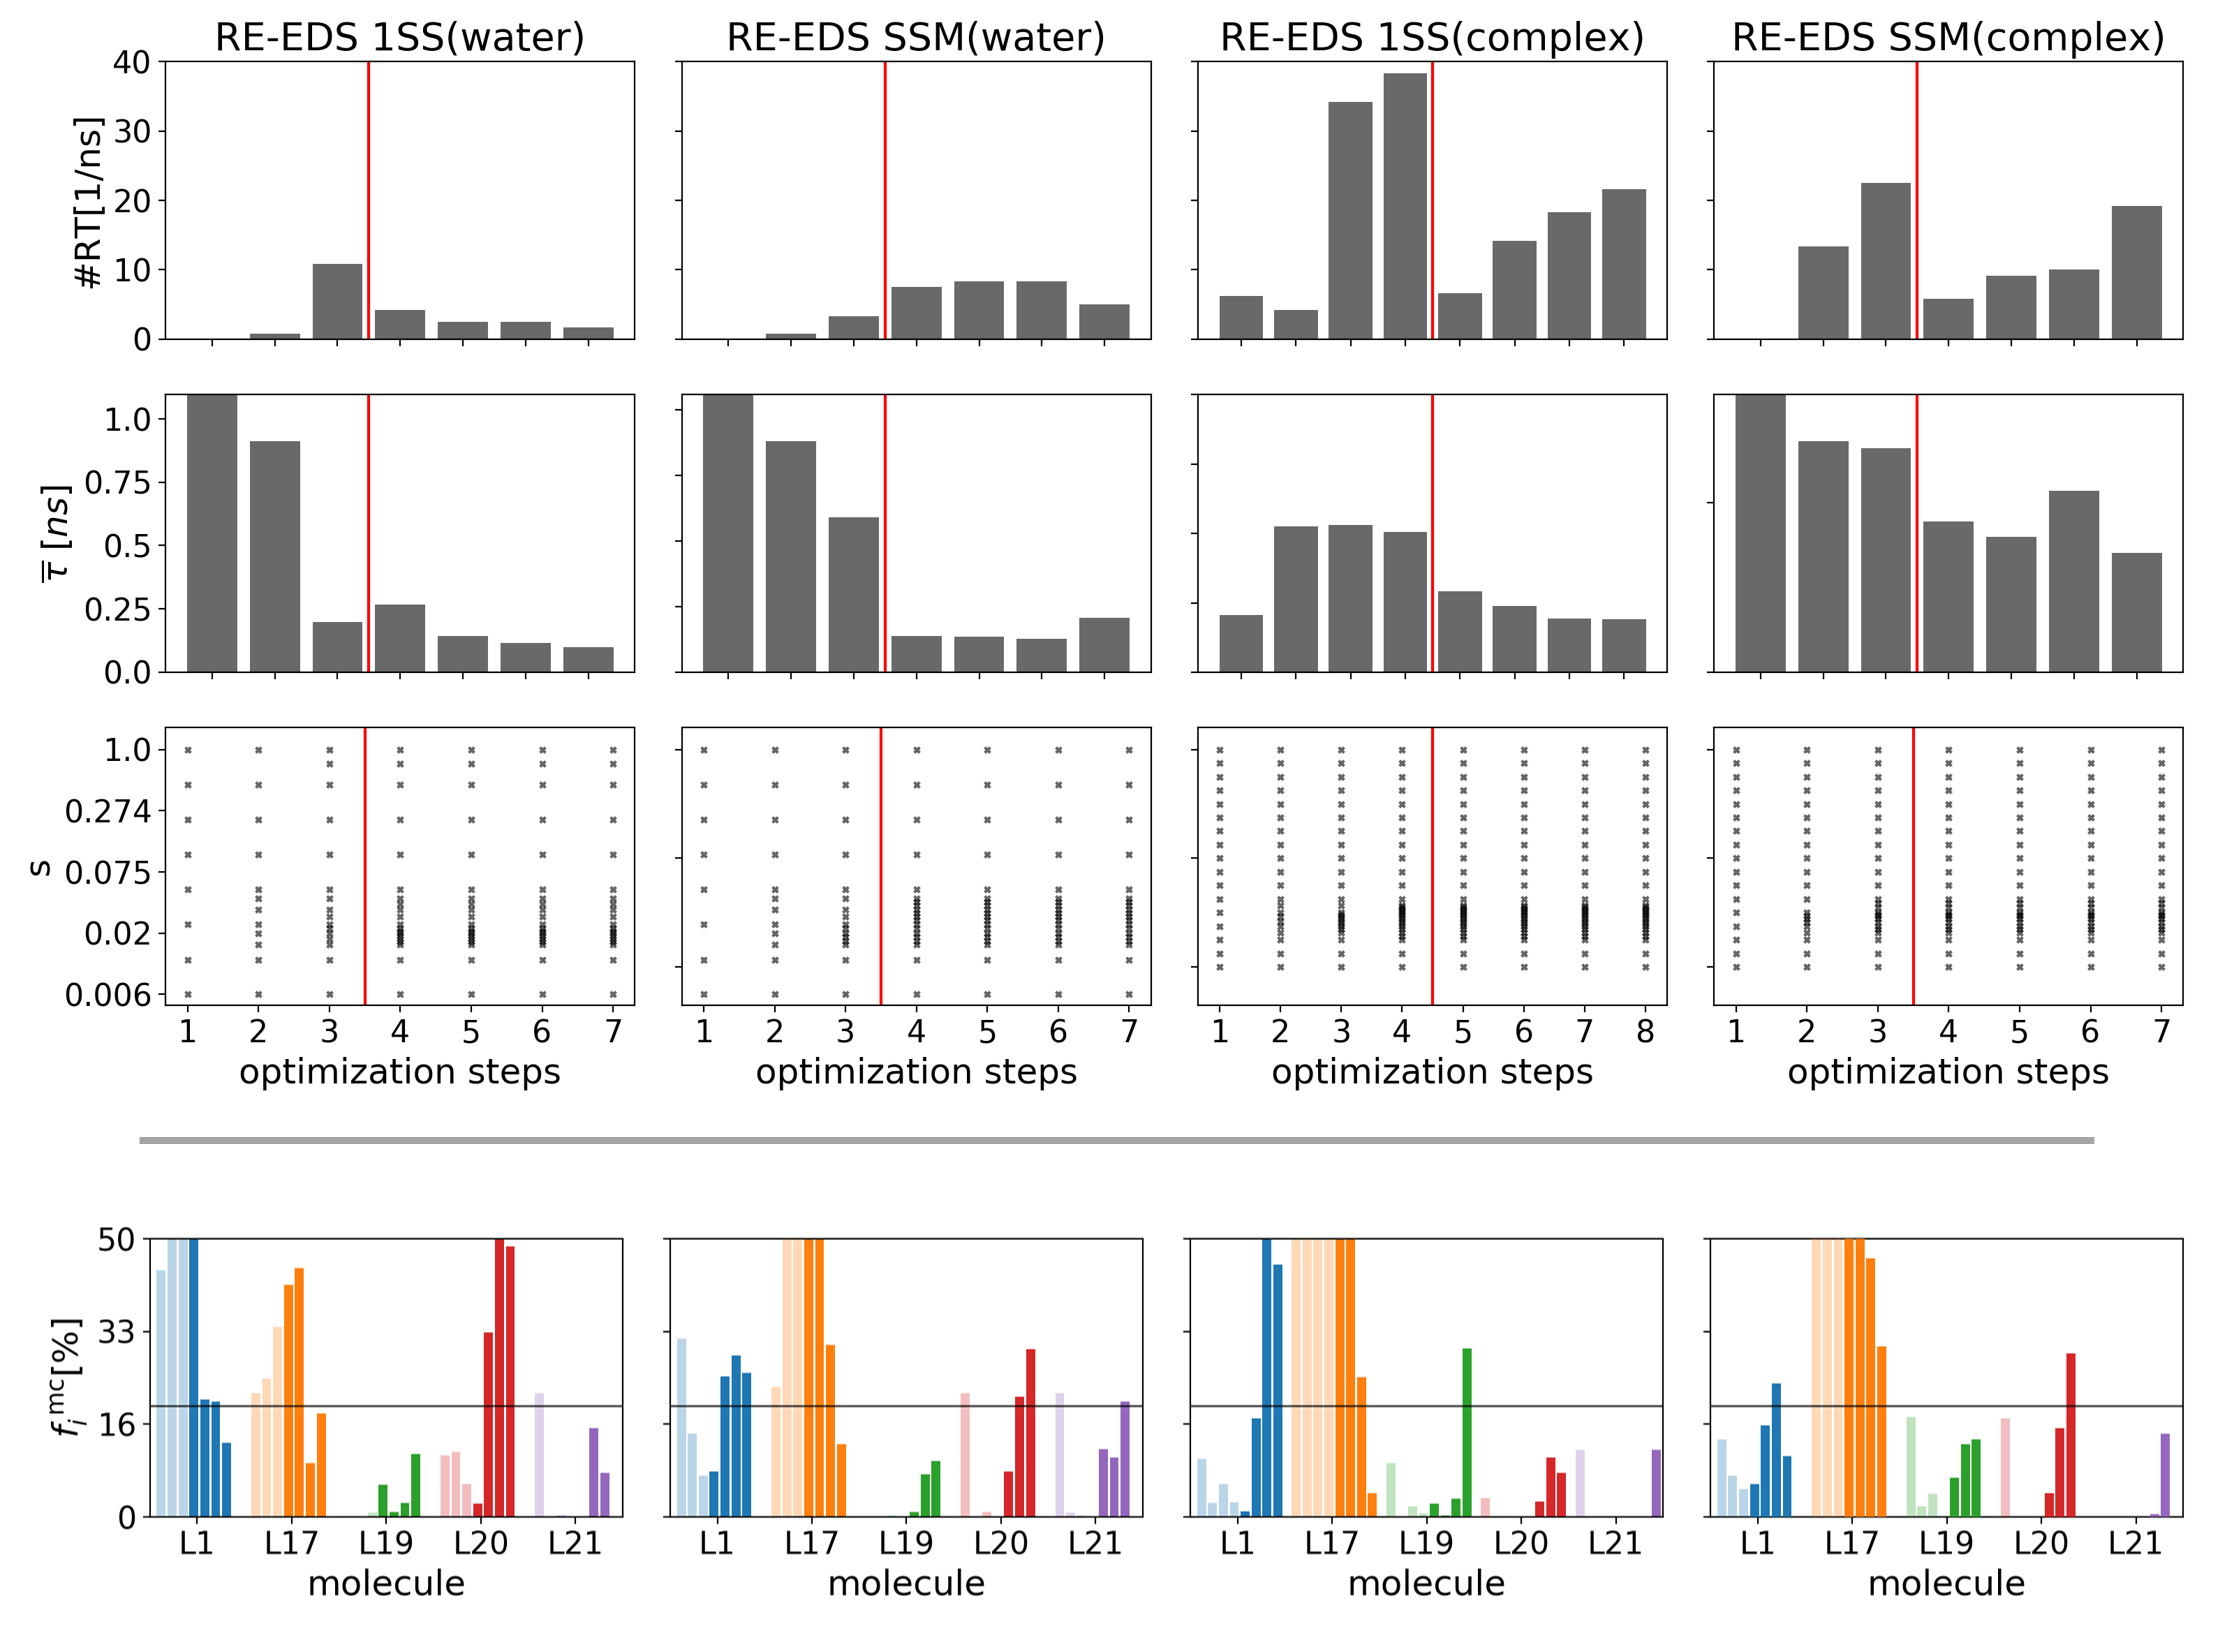
\includegraphics[width=\textwidth]{fig/results/ringOpening/paramOptimization/S-optimization_ringOpening.png}
\caption{Optimization steps of the $s$-distribution with the N-LRTO \cite{Sidler2017} algorithm followed by the energy offset rebalancing scheme (start indicated by the red horizontal line). The measured quality criteria were the number of round trips (1. row), the average round-trip time $\overline{\tau}$ (2. row), the placement of the replicas in $s$-space (3. row), and the sampling fractions of maximally contributing states $f_{i}^{\text{mc}}$ (4. row). The light colored bars of $f_{i}^{\text{mc}}$ indicate $s$-optimization iterations, whereas the fully colored bars indicate energy offset rebalancing steps. }
\label{fig: CHK1_RingOpening_sOptimization}
\end{figure}



%% tau converge - Conclusion
The $s$-optimization was stopped after a sufficiently high number of round trips and low round-trip time was reached. 
This resulted in 20 replicas for the ligands in water after three $s$-optimization iterations.
For the protein-ligands complex, the fourth $s$-optimization iteration was chosen for the 1SS approach, and the third iteration for the SSM approach, resulting in 29 and 25 replicas, respectively. 
The average round-trip time after convergence was $\overline{\tau} = 0.4 \pm 0.2$~ns for all simulations.

After the $s$-optimization, the energy offset rebalancing scheme was applied to improve the state sampling. 

%RT analysis
During the rebalancing steps, no further replicas were added to the $s$-distribution. It is essential for the success of the rebalancing scheme that round trips occur. Therefore, the number of round trips and average round-trip time were monitored. In all systems, the number of round trips and $\overline{\tau}$ remained relatively stable over the four rebalancing steps. For the RE-EDS 1SS approach in water, the number of round trips slightly decreased but never dropped to zero.

%% states sampling
Across the optimization steps, also the sampling of the end states as maximally contributing states at $s=1.0$ was monitored.
During the $s$-optimization, some end states ``vanish'' and are no longer sampled as maximal contributing states. This leakage effect can occur when the initially estimated $E^{\text{R}}$ are not exactly optimal \cite{Sidler2016}. 
With energy offset rebalancing, the sampling of each end state can be recovered, and the sampling distribution approaches the ideal case.
%After the s-optimization the MAE($P^{\text{maxContrib}}$) was for all approaches approximately at $25\%$, with the exception of the 1SS water system, here it was $20\%$. 
After rebalancing, all end states showed a $f_i^{\text{mc}} > 0$ and the mean absolute deviation of the sampling distribution from ideal decreased from $20-25\%$ to approximately $7-12\%$ (Figure S4 in the Supporting Information). % SUPPL
 
\subsection{Free-Energy Calculation}
After successfully optimizing the RE-EDS parameters, the production runs were performed for $3.5$~ns. 

%%Sampling++
Both in water and in complex, the potential-energy distributions of the end states generally match well the corresponding distributions from the standard MD simulations of the single end states (Figure \ref{fig:RingOpening_sampling_comparison}). Only in the complex 1SS approach, a deviation can be seen for L17, with a slight shift to higher potential energies. This is due to insufficient sampling of L17 in this case (see below). 
%
The analysis of the maximally contributing end states at $s=1.0$ shows that in water all end states were sampled close to the ideal equal distribution (Figure S5 in the Supporting Information). % SUPPL
In the simulation of the protein-ligands complex, there are still differences in sampling. Especially with the 1SS approach, L19 is generally sampled too much, while L17 is not sampled enough. The situation is improved with the SSM approach.
Comparing $f_i^{\text{occur}}$ and $f_i^{\text{mc}}$ in Figure S5 indicates that the end states in the CHK1 system are clearly separated (i.e. no phase-space overlap). % SUPPL

\begin{figure}[h]
    \centering
    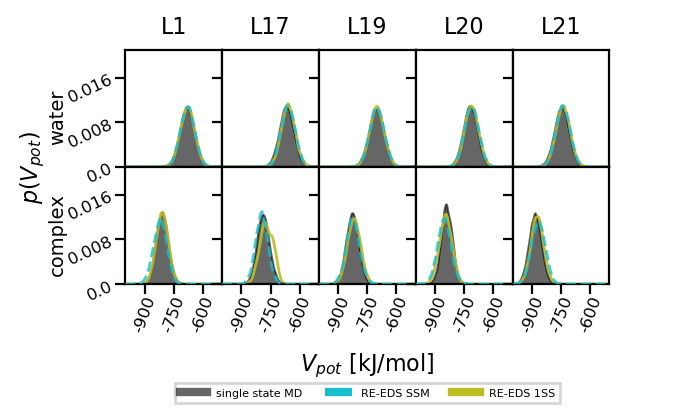
\includegraphics[width=\columnwidth]{fig/results/ringOpening/FE/RingClosure_system_final_sampling.png}
    \caption{Comparison of the Boltzmann reweighted potential-energy distributions obtained from standard MD simulations of a given end state (black) and from the RE-EDS production runs of the 1SS (green) and SSM (turquoise, dashed) approaches.}
    \label{fig:RingOpening_sampling_comparison}
\end{figure}

%%Accuracy
From the replica at $s=1.0$, the free-energy differences were calculated using Eq.~(\ref{EQ: Free Energy calculation via reference state}) and the resulting $\Delta \Delta G^\text{bind}_{ji}$ were compared with the experimental results taken from Ref.~\cite{Huang2012}. The results are shown graphically in Figure \ref{fig:CHK1_set2_FreeEnergyCalculation} and numerically in Table \ref{tab: RE-EDS_FE_RingCycleOpening_ddF}. The individual free-energy differences are given in Table S3 in the Supporting Information. %SUPPL
The RMSE with RE-EDS 1SS is $4.4$~kJ~mol$^{-1}$ and the MAE is $3.9\pm2.8$~kJ~mol$^{-1}$. 
%
%how I calculate the MAE and RMSD:
%MAE = np.mean(np.abs(ddG_differences))
%std(MAE) = np.std(np.abs(ddG_differences)) #gives an impression of absolute deviation of all ddG_diffs
%RMSE = np.sqrt(np.mean(np.square(ddG_differences))
%
The main deviations stem from ligand L17 in the RE-EDS 1SS approach, which can be explained by the insufficient sampling of L17 in the complex (see Figure \ref{fig:RingOpening_sampling_comparison} and Figure S5 in the Supporting Information). %SUPPL

The performance was substantially improved using the SSM approach with RE-EDS, giving an RMSE of $3.3$~kJ~mol$^{-1}$ and an MAE of $2.8 \pm 1.7$~kJ~mol$^{-1}$. 
Only two values (L21-L11) and (L21-L19) deviate more than $4.184$~kJ~mol$^{-1}$ (i.e. $1$~kcal~mol$^{-1}$) from experiment.
The Spearman correlation coefficient for RE-EDS 1SS is $r_{\text{Spearman}}=0.01$ and for RE-EDS SSM $r_{\text{Spearman}}=0.69$.

%%Performance:
Next, we assessed the convergence of the $\Delta G_{ji}$ values as a function of simulation time (Figure S6 in the Supporting Information). % SUPPL
For the RE-EDS 1SS approach, all free-energy differences appeared converged after $2.5$~ns in water and after $2.7$~ns in the complex. For the RE-EDS SSM approach, convergence was observed after $2.5$~ns in water and after $2.9$~ns in the complex.

\begin{figure}[h]
    \centering
    \begin{subfigure}{0.85\columnwidth}
        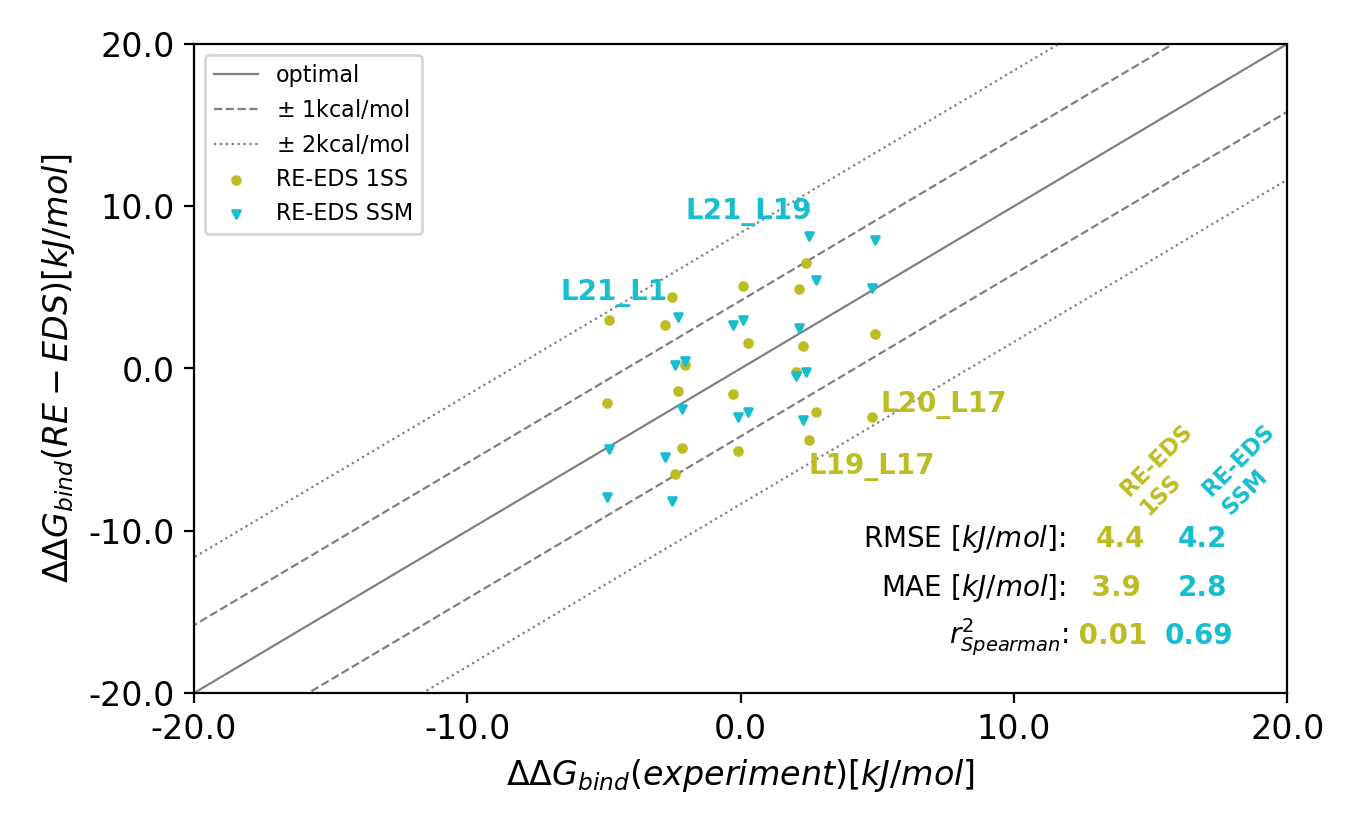
\includegraphics[width=\textwidth]{fig/results/ringOpening/FE/RingClosure_system_final_results_4ns_comparison.png}
        \end{subfigure}
    \begin{subfigure}{0.85\columnwidth}
        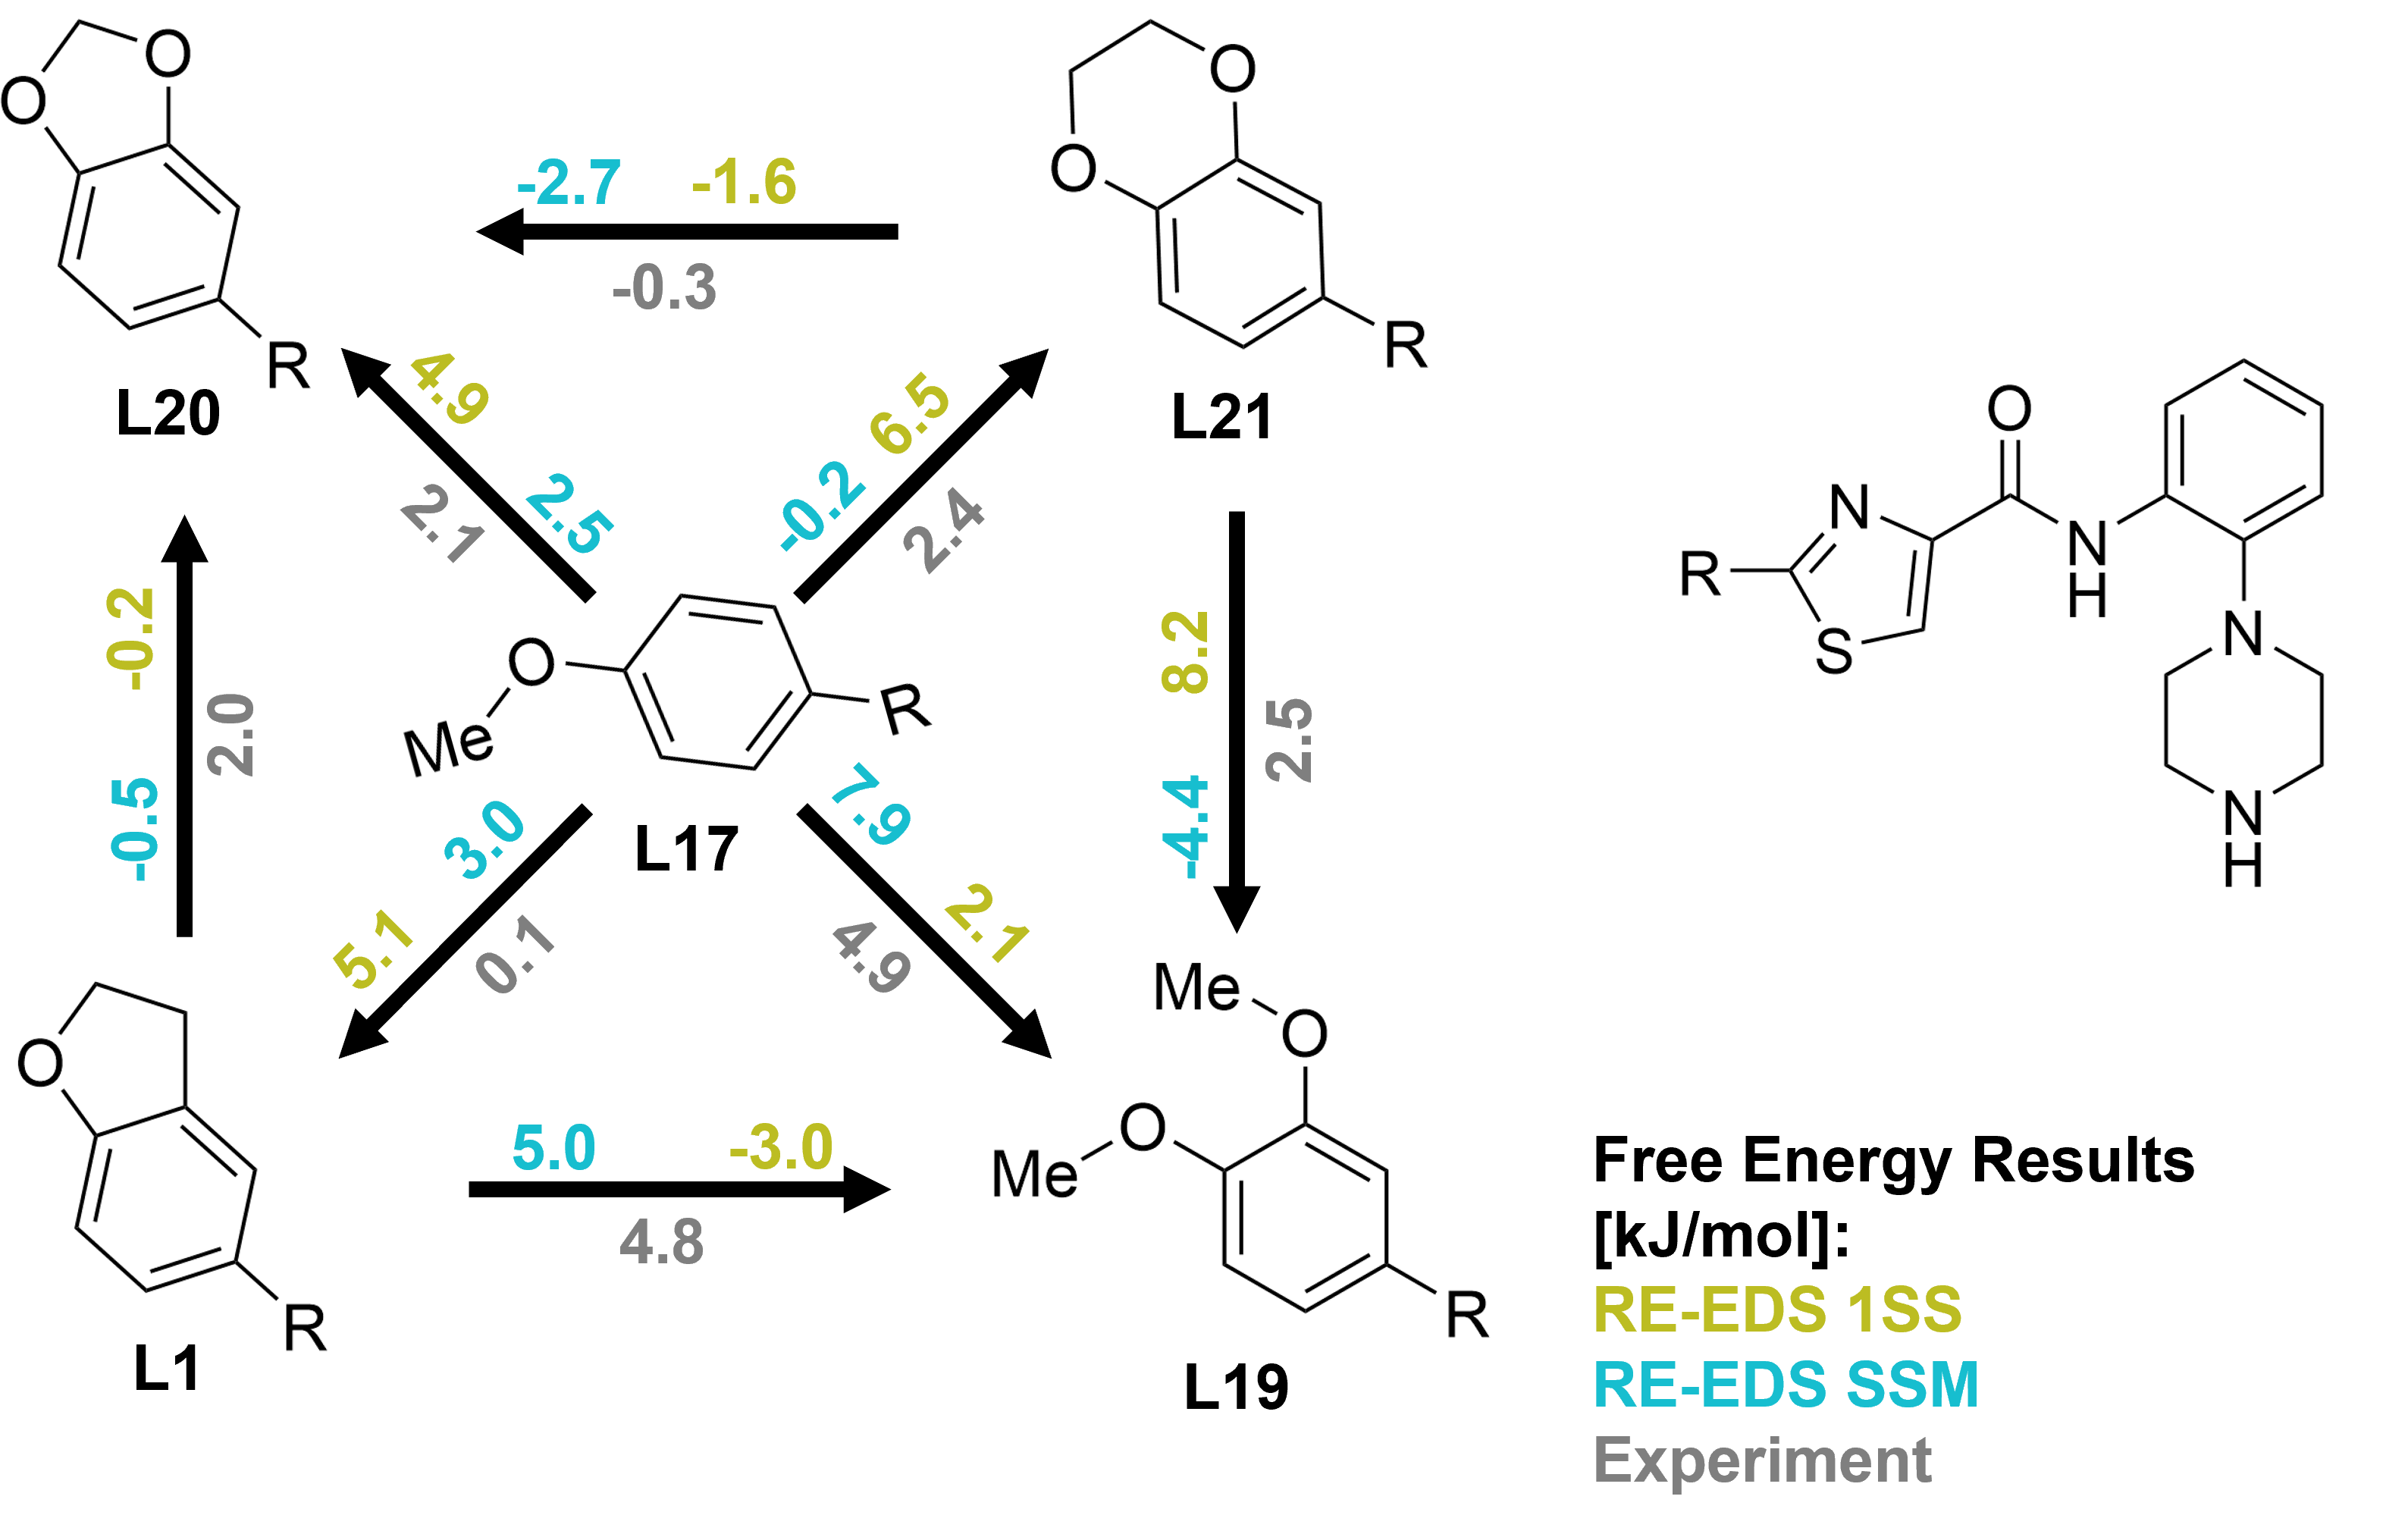
\includegraphics[width=\textwidth]{fig/results/ringOpening/FE/ddG_bind_paper_comparison_reeds_only_4nsSimulation.png}
        \end{subfigure}
    \caption{Free-energy differences estimated from the production run of $3.5$~ns length. (Top): Comparison between the experimental and calculated $\Delta \Delta G^\text{bind}_{ji}$ using RE-EDS 1SS and RE-EDS SSM. The results were calculated with all possible pairwise transformations (forward and backward). (Bottom): Graphical representation of the $\Delta \Delta G^\text{bind}_{ji}$ results with structures, inspired by the one in Ref.~\cite{Wang2017}.}
    \label{fig:CHK1_set2_FreeEnergyCalculation}
\end{figure}

%Comparison results with Schroedinger & Jespers
By applying the RE-EDS methodology to the same system of five CHK1 inhibitors as studied by Wang \textit{et. al.} \cite{Wang2017} and later on also Jespers \textit{et al.} \cite{Jespers2019}, a direct comparison with FEP+ and QligFEP is possible (Table \ref{tab: RE-EDS_FE_RingCycleOpening_ddF}). Note that the quality metrics were calculated over all possible pairs of ligands and in both directions, not only those directly calculated by FEP+ and QligFEP.
For FEP+, we obtained an RMSE of $2.4$~kJ~mol$^{-1}$ and an MAE of $1.8 \pm 1.2$~kJ~mol$^{-1}$ with a Spearman correlation coefficient of $r_{\text{Spearman}}=0.67$.
Including cycle closure correction (CC) \cite{Wang2017} reduced the RMSE to $2.1$~kJ~mol$^{-1}$ and the MAE to $1.9 \pm 1.0$~kJ~mol$^{-1}$. The Spearman correlation coefficient increased to $r_{\text{Spearman}}=0.73$.
Jespers \textit{et al.} \cite{Jespers2019} reported free-energy differences with QligFEP as an average over ten independent replicas, each with significantly less simulation time per $\lambda$-window than in Ref.~\cite{Wang2017}. For QligFEP, an RMSE of $2.3$~kJ~mol$^{-1}$, an MAE of $2.0 \pm 1.2$~kJ~mol$^{-1}$, and a Spearman coefficient of $r_{\text{Spearman}}=0.61$ was obtained.

Overall, the performance of RE-EDS SSM is comparable with the pairwise methods. The results with FEP+ CC and QligFEP showed a slightly higher accuracy compared to experiment, likely due to the different force fields used. The Spearman correlation coefficient is comparable with the other methods for the RE-EDS SSM approach.

\begin{table}[h]
\caption{Relative binding free energies $\Delta \Delta G^\text{bind}_{ji}$ from experiment and calculated with the RE-EDS 1SS and RE-EDS SSM approaches. For comparison, the results for FEP+ with and without cycle closure (CC) correction taken from Ref.~\cite{Wang2017} and the results for QligFEP taken from Ref.~\cite{Jespers2019} are listed. The free-energy differences of directly simulated paths were used to infer not directly simulated free-energy differences (marked in bold). If multiple indirect paths were possible, their average was used. The errors for QligFEP were determined in Ref.~\cite{Jespers2019} by calculating the standard deviation over ten replicas. For FEP+, the error of the results was taken from the used BAR \cite{Bennett1976} method and the FEP+ CC errors were obtained from the cycle closure analysis. For the RE-EDS approaches, the reported error is based on the statistical uncertainties of the $\Delta G_{ji}^{env}$ values estimated using Gaussian error approximation \cite{Christ2008}. The uncertainty estimate of the RMSE was obtained by a 100-fold bootstrapping approach. }
\begin{center}
\footnotesize
\resizebox{\columnwidth}{!}{%
\begin{tabular}{ c c |c |c|c|c|c|c}
  \multicolumn{2}{c|}{Ligands} & \multicolumn{1}{c|}{Exp. \cite{Huang2012}} &\multicolumn{1}{c|}{FEP+ \cite{Wang2017}}&\multicolumn{1}{c|}{FEP+ CC \cite{Wang2017}}&\multicolumn{1}{c|}{QligFEP \cite{Jespers2019}}&\multicolumn{1}{c|}{RE-EDS 1SS}&\multicolumn{1}{c}{RE-EDS SSM}\\ 
    $i$ & $j$  & [kJ~mol$^{-1}$]  & [kJ~mol$^{-1}$] & [kJ~mol$^{-1}$] & [kJ~mol$^{-1}$] & [kJ~mol$^{-1}$] & [kJ~mol$^{-1}$]  \\
  \hline
        L17 &  L1 &   0.1 & -3.6 $\pm$ 0.4          & -2.9 $\pm$ 1.0         & -1.6 $\pm$ 1.7                                     &    5.1 $\pm$ 0.8 &  3.0 $\pm$ 2.0 \\
        L19 &  L1 &  -4.8 & -3.9 $\pm$ 0.3          & -4.0 $\pm$ 0.6         & -1.7 $\pm$ 2.0                                     &    3.0 $\pm$ 1.0 & -5.0 $\pm$ 0.1\\
        L20 &  L1 &  -2.0 & -2.5 $\pm$ 0.1          & -3.1 $\pm$ 1.0         & -1.3 $\pm$ 1.3                                     &    0.2 $\pm$ 0.9 &  0.5 $\pm$ 0.1\\
        L21 &  L1 &  -2.3 &\textbf{-3.4} $\pm$ \textbf{0.7}  &\textbf{-3.2} $\pm$ \textbf{1.3} & \textbf{-0.1} $\pm$ \textbf{3.5} &   -1.4 $\pm$ 0.8 &  3.2 $\pm$ 0.1\\
        L19 &  L17 & -4.9 & -1.4 $\pm$ 0.3          & -1.1 $\pm$ 1.0         & \textbf{0.1} $\pm$ \textbf{2.6}                    &   -2.1 $\pm$ 0.6 & -7.9 $\pm$ 1.9\\
        L20 &  L17 & -2.1 &  0.3 $\pm$ 0.4          & -0.1 $\pm$ 0.8         & -1.3 $\pm$ 2.3                                     &   -4.9 $\pm$ 0.1 & -2.5 $\pm$ 1.9\\
        L21 &  L17 & -2.4 & -1.1 $\pm$ 0.4          & -0.9 $\pm$ 0.9         &\textbf{0.7} $\pm$ \textbf{2.6}                     &  -6.5 $\pm$ 0.1 &  0.2 $\pm$ 1.9\\
        L20 &  L19 & 2.8  &\textbf{0.8} $\pm$ \textbf{0.6}   & \textbf{0.1} $\pm$ \textbf{1.3} & \textbf{-0.4} $\pm$ \textbf{3.7} &  -2.7 $\pm$ 0.6 &  5.4 $\pm$ 0.1\\
        L21 &  L19 & 2.5  & -0.1 $\pm$ 0.6         &  0.6 $\pm$ 0.1         &  0.6 $\pm$ 4.9                                      &  -4.4 $\pm$ 0.6 &  8.2 $\pm$ 0.1\\
        L21 &  L20 & -0.3 & -0.3 $\pm$ 0.8         & -0.6 $\pm$ 0.8         &  0.6 $\pm$ 1.1                                    &    -1.6 $\pm$ 0.1 &   -2.7 $\pm$ 0.1\\ 
    \hline
        \multicolumn{2}{c|}{RMSE} &                    & 2.4  $\pm$ 0.3           & 2.1  $\pm$ 0.2          &  2.3  $\pm$ 0.38      & 4.4 $\pm$ 0.5         & 3.3  $\pm$ 0.3 \\
        \multicolumn{2}{c|}{MAE} &                     & 1.8 $\pm$ 1.2 & 1.9 $\pm$ 1.0 & 2.0 $\pm$ 1.2 & 3.9 $\pm$2.8 & 2.8 $\pm$ 1.7 \\
        %\multicolumn{2}{c|}{$r_{\text{Pearson}}$} & & 0.66            & 0.67          & 0.63          & -0.07m          & 0.71 \\
        \multicolumn{2}{c|}{$r_{\text{Spearman}}$} & & 0.67           & 0.73          & 0.61          & 0.01           & 0.69 \\
        \multicolumn{2}{c|}{$t_{simulation} [ns]$} & & 640          &  640         &  51        & 171.5         & 157.5  \\
\end{tabular}
}
\end{center}
\label{tab: RE-EDS_FE_RingCycleOpening_ddF}
\end{table}

% 
%FEP+: 
%MAE 1.99 +- 1.4
%RMSE 2.43
%r pearson 0.56 	 r spearman 0.56
%
%FEP+ CC: 
%MAE 1.88 +- 1.05
%RMSE 2.15
%r pearson 0.66 	 r spearman 0.71

%QLigFEP
%MAE 1.97 +- 1.2
%RMSE 2.3
%r pearson 0.63 	 r spearman 0.61


%ComputationalCost
%FEP: 16 l-windwos*5ns*4 pairs * 2 approaches ==> 640ns
%QligFEP: 10 repetitions * (eq 131ps + 51lams * 10ps sim) * 4 pairs * 2 approaches ==> 51ns
%Complex: 
%	- Optimization: 1ns * 17 Eoff + 0.5ns*17 sopt1 + 1ns*21 sopt2 + 3*0.5ns*25 eoffRB = 84ns
%	- Production: 25*3.5 = 87.5ns / 29*3.5 =  101.5
%Water:
%	- Optimization: 1ns * 12 Eoff + 0.5ns*12 sopt1 + 1ns*16 sopt2 + 3*0.5ns*20 eoffRB = 64ns
%   - Production: 20 * 3.5maybe = 70ns
%old reeds line complex - optim: eoff(21*0.8)+sop1(0.4ns*21)+sopt2(0.8ns*25)+sopt3(1.2ns*29)+sopt4(1.2ns*31)+sopt5(1.2ns*35) = 276.4 ns
%old reeds line complex - prod: 4ns*41 = 164 ns
%new reeds line complex - optim: eoff(21*0.8)+sop1(0.4ns*21)+sopt2(0.8ns*25)+sopt3(1.2ns*29)+eoffRB(0.5ns*2*29) = 122 ns
%new reeds line complex - prod: 4ns*29 = 116ns 

In terms of computational cost, the RE-EDS approach (with $3.5$~ns per replica) resulted in about a quarter of the total simulation time (in ns) than reported for the FEP+ calculations in Ref.~\cite{Wang2017} (Table \ref{tab: RE-EDS_FE_RingCycleOpening_ddF}). However the QligFEP approach is the approach with the lowest simulation time consumption. A major advantage of the simultaneous simulation of multiple ligands in a single RE-EDS simulation is that all $N(N-1)/2$ transformations are sampled directly, leading to low statistical errors and removing the need for a state graph. This advantage increases with increasing number of ligands. The current workflow of RE-EDS uses a relatively large amount of simulation time for parameter optimization. Future work will focus on further optimization of the workflow to reduce the pre-processing time. 

From the calculated relative binding free energies, $\Delta G_{i}^{\text{bind}}$ can be obtained by using one experimental value as anchor point. This allows us to generate a ranking of the five ligands. To avoid any bias from the selected experimental anchor point, all possibilities were calculated and the resulting values averaged (Table \ref{tab:RE-EDS_FE_RingCycleOpening_absoluteShiftDF}). While the RMSE is generally low for all approaches ($<$ 1 kcal mol$^{-1}$ = 4.184 kJ mol$^{-1}$), the ranking of the ligands as measured by $r_{\text{Spearman}}$ is not very good. 
%A strong correlation with experiment is of interest in drug design approaches, as the ranking of ligands in virtual screening is important to suggest the most promising drug candidates to be synthesized.
This observation is not uncommon for ligand series with small differences in binding free energy \cite{Wang2015,Schindler2020}.
Note that the uncertainties of the individual values have increased compared to the relative binding free energies due to the anchoring and averaging procedure.

\begin{table}[h]
\caption{Absolute binding free energies $\Delta G_{i}^{\text{bind}}$ and ranking of the ligands derived from the relative binding free energies. The values were calculated from the relative binding free energies using an experimental binding free energy as anchor point, and then averaged over the five possibilities. The errors are standard deviations over the possible outcomes. For comparison, the results for FEP+ with and without cycle closure (CC) correction taken from Ref.~\cite{Wang2017} and the results for QligFEP taken from Ref.~\cite{Jespers2019} are shown (calculated with the same procedure). The uncertainty estimate of the RMSE was obtained by a 100-fold bootstrapping approach.}
\begin{center}
\footnotesize
\resizebox{\columnwidth}{!}{%
\begin{tabular}{ c |c |c|c|c|c|c}
  Ligands & \multicolumn{1}{c|}{Exp. \cite{Huang2012}} &\multicolumn{1}{c|}{FEP+ \cite{Wang2017}}&\multicolumn{1}{c|}{FEP+ CC \cite{Wang2017}}&\multicolumn{1}{c|}{QligFEP \cite{Jespers2019}}&\multicolumn{1}{c|}{RE-EDS 1SS}&\multicolumn{1}{c}{RE-EDS SSM}\\ 
    Molecule & [kJ~mol$^{-1}$]  & [kJ~mol$^{-1}$] & [kJ~mol$^{-1}$] & [kJ~mol$^{-1}$] & [kJ~mol$^{-1}$] & [kJ~mol$^{-1}$]  \\
  \hline
        L1 &   -40.7 & -41.7 $\pm$ 1.7         & -41.7 $\pm$ 0.9         & -38.5 $\pm$ 1.5 &   -40.0 $\pm$ 3.4 &    -38.0 $\pm$ 2.0 \\
        L17 &  -40.8 &  -38.0 $\pm$ 1.0         & -38.2 $\pm$ 1.1         & -38.6 $\pm$ 1.3 &    -33.7 $\pm$ 1.3 & -41.7 $\pm$ 2.3 \\
        L19 &  -35.9  & -38.1 $\pm$ 0.9         & -38.3 $\pm$ 1.8         & -38.3 $\pm$ 1.0 &   -37.6 $\pm$ 3.3 &  -33.0 $\pm$ 2.0 \\
        L20 &  -38.6 & -38.6  $\pm$ 1.6         & -38.3 $\pm$ 1.4         & -39.2 $\pm$ 1.7 &    -40.4 $\pm$ 3.3 & -39.1 $\pm$ 2.3 \\
        L21 &  -38.4 & -37.7  $\pm$ 1.4         & -37.8 $\pm$ 1.3         & -39.4 $\pm$ 1.9 &    -42.4 $\pm$ 2.9 &    -42.5 $\pm$ 1.4 \\
    \hline
        RMSE &                    & 1.7  $\pm$  0.4        & 1.7   $\pm$ 0.4        & 1.7 $\pm$ 0.4          & 3.8 $\pm$ 1.3         & 2.6 $\pm$ 0.6 \\
        MAE &                     & 1.3 $\pm$ 1.0  & 1.4 $\pm$ 0.9 & 1.4 $\pm$ 0.9 & 3.0 $\pm$ 2.3 & 2.2 $\pm$ 1.6 \\
        $r_{\text{Spearman}}$ &  & 0.20           & 0.10          & -0.21         &  -0.40           & 0.30 \\
\end{tabular}
}
\end{center}
\label{tab:RE-EDS_FE_RingCycleOpening_absoluteShiftDF}
\end{table}



%%% MERGE APPENDIX %%%

\section{Parameter Exploration}
A fast transition of the initial maximally contributing end state to the desired maximally contributing end state was observed by monitoring the maximally contributing end state over time.
The transition occurred latest after $0.5$~ns, and the system remained in the biased end state for the rest of the simulation time.
In both water and complex simulations, the desired end state was sampled about $~99\%$ of the simulation time with the exception of L19 in water (Table \ref{SItab:RingCycleOpenin_sampling_fraction_optimizedStates}).
To inspect if the optimized state simulations' results sufficiently represent the target states, a comparison between the target state obtained potential-energy distributions in the EDS simulations with MD simulations consisting of only the target state was conducted (Figure \ref{fig:CHK1_set2_stateOptimization_EnergyDistribution}). 

\begin{table}[H]
\centering
\caption{Fraction of the simulation time $f_i^{\text{mc}}$ (in \%) that the desired end state was sampled as the maximally contributing state during the EDS simulation to optimize the coordinates for a desired end state.}
\label{SItab:RingCycleOpenin_sampling_fraction_optimizedStates}
\begin{tabular}{ l | c c }
 Ligand & Water  & Complex \\ 
 \hline
     L1 & 99.84 & 99.97 \\ 
     L17 & 99.99 & 99.97\\
     L19 & 36.07 &  99.98\\
     L20 & 99.99 & 100\\
     L21 & 100 & 99.97 \\
\end{tabular}
\end{table}

\begin{table}[H]
\centering
\caption{Potential thresholds for occurrence sampling ($T_{i}^{\text{phys}}$) and undersampling ($T_{i}^{\text{us}}$) determined during the parameter exploration (in kJ~mol$^{-1}$).}
\label{SItab:RingCycleOpenin_PotentialTresholds}
\begin{tabular}{ l | c c |c c| }
 Ligand &\multicolumn{2}{c|}{Water} & \multicolumn{2}{c|}{Complex}\\ 
  & \multicolumn{1}{c}{$T^{\text{phys}}$}& \multicolumn{1}{c|}{$T^{\text{us}}$}&  \multicolumn{1}{c}{$T^{\text{phys}}$}& \multicolumn{1}{c|}{$T^{\text{us}}$} \\ 
 \hline
     L1  & -582.96 & -436.05 & -737.37 & -516.41\\ 
     L17 & -572.41 & -419.16 & -717.95 & -492.83\\
     L19 & -579.13 & -415.91 & -738.95 & -483.78\\
     L20 & -636.00 & -492.75 & -759.01 & -549.35\\
     L21 & -656.22 & -488.43 & -805.30 & -539.78\\
\end{tabular}
\end{table}

\begin{figure}[H]
\centering
     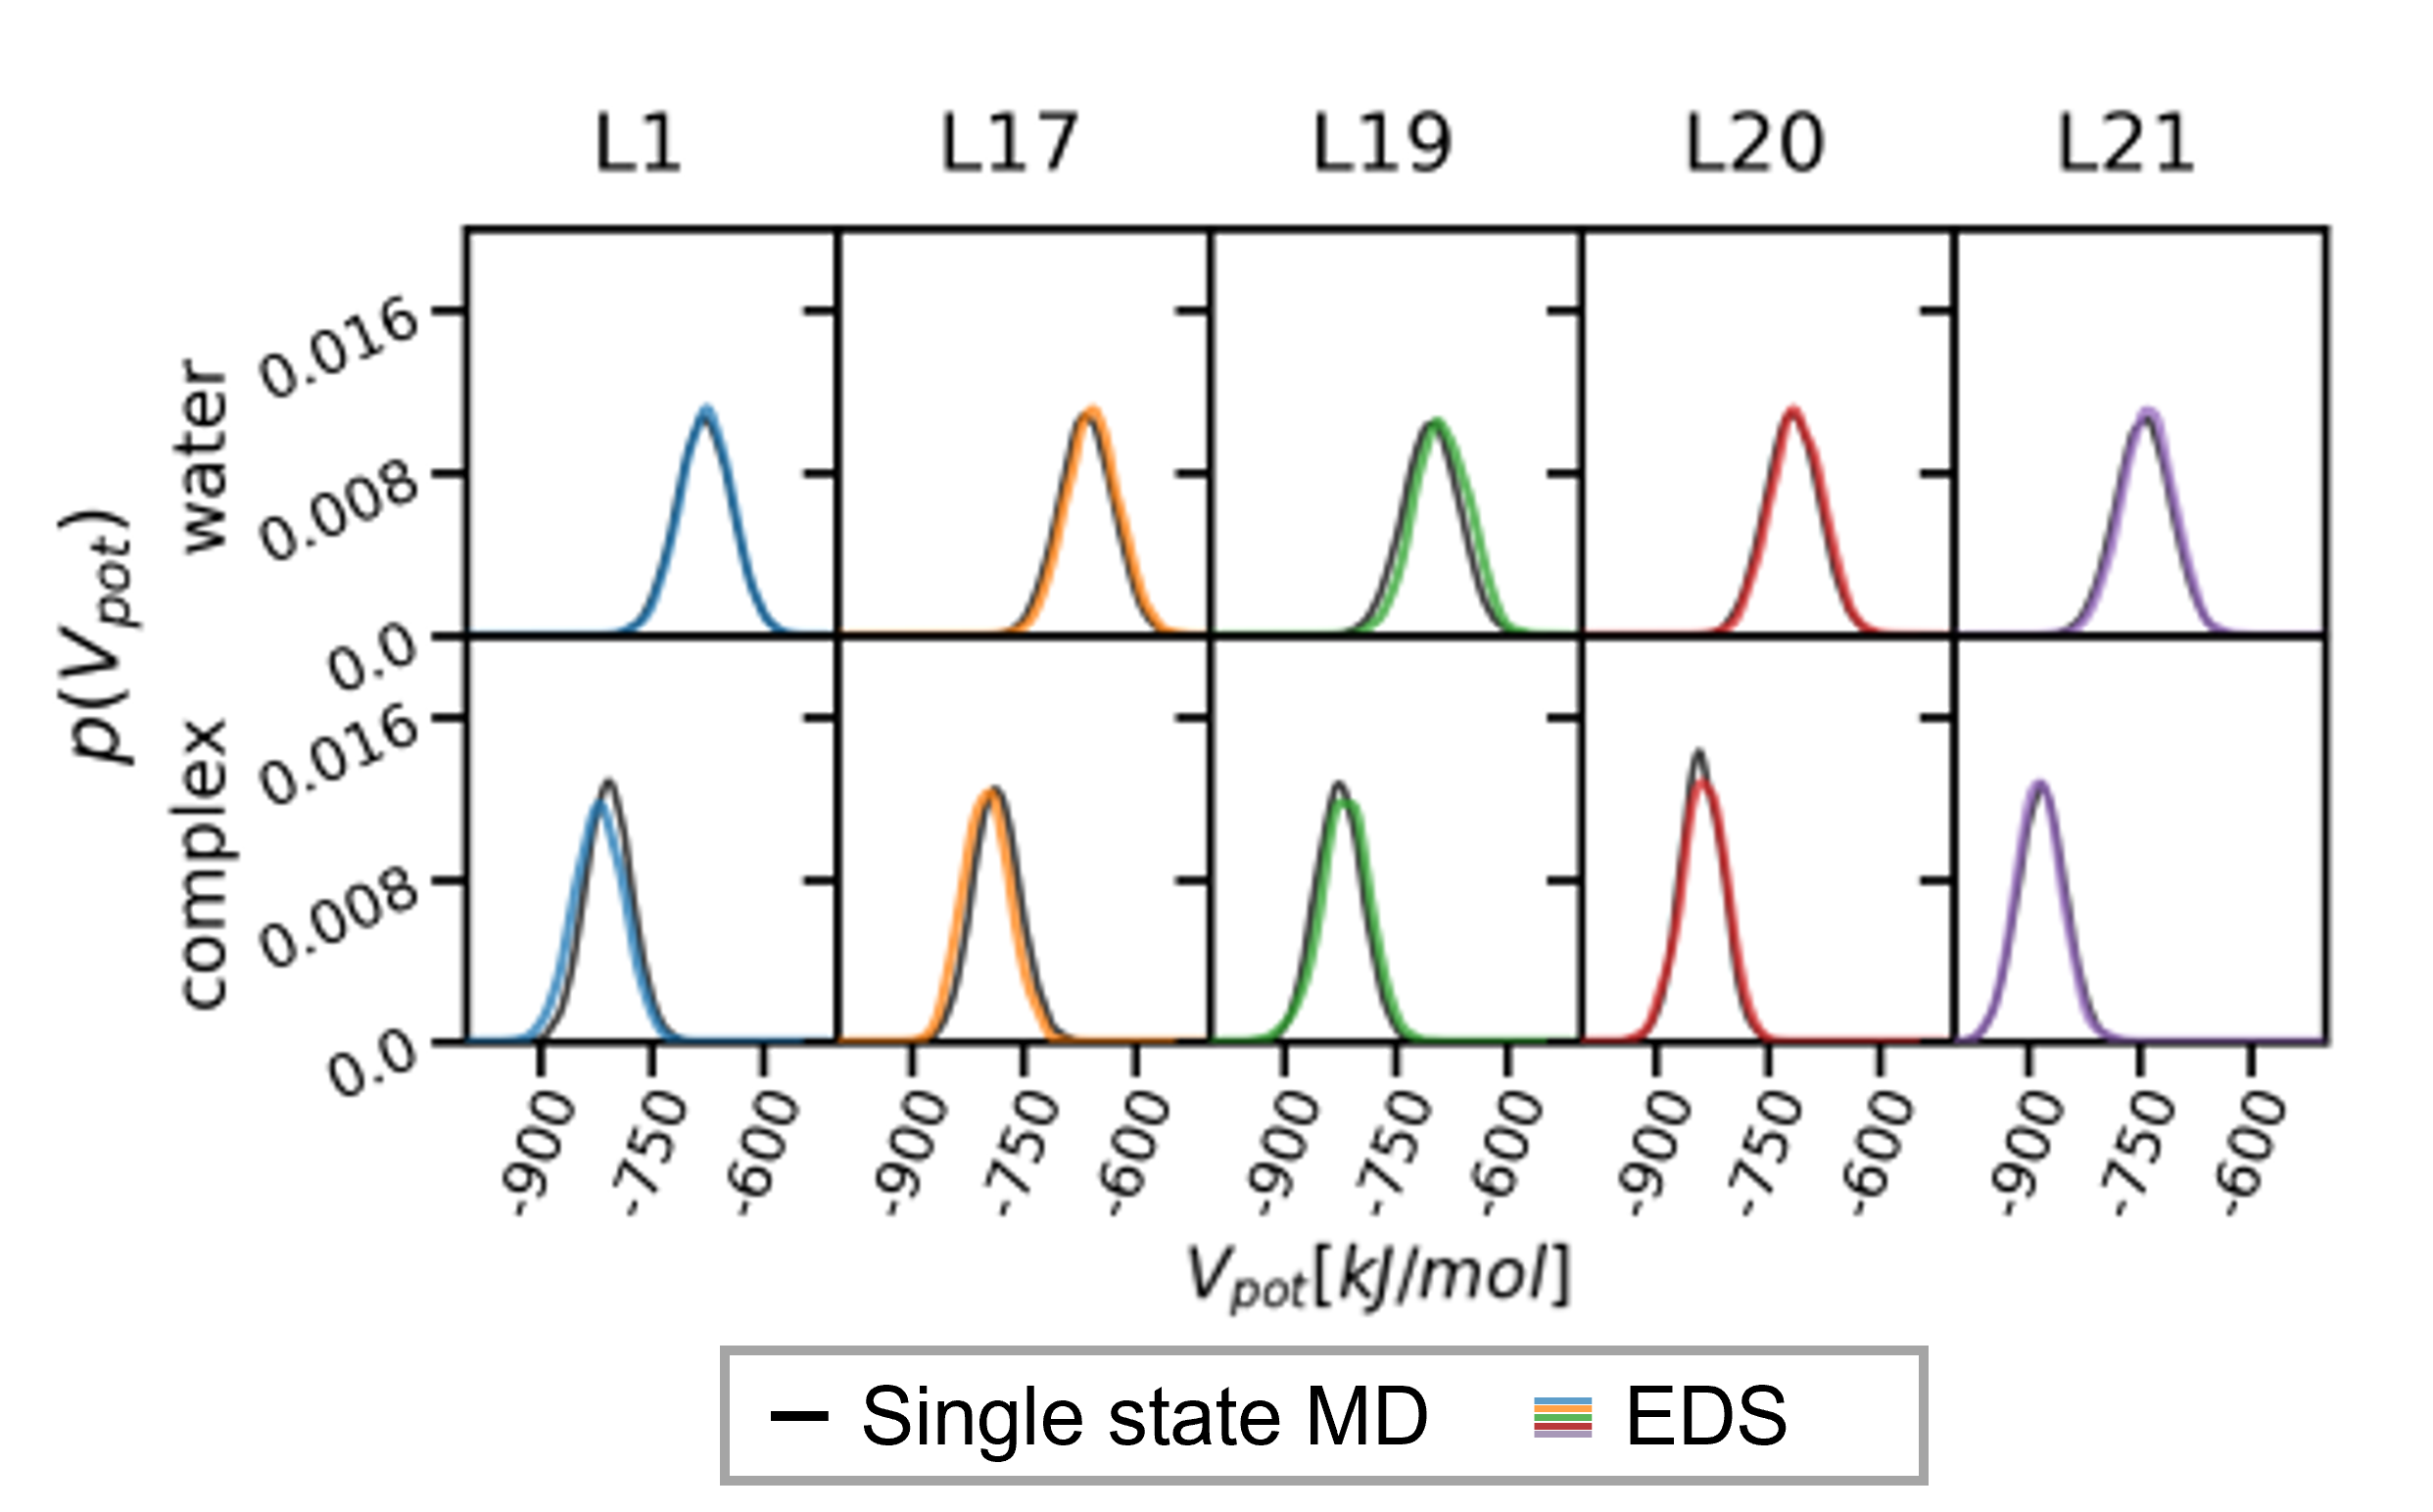
\includegraphics[width=0.8\textwidth]{fig/results/ringOpening/paramExploration/single_state_energy_sampling.png}
    \caption{Comparison of the potential-energy distribution obtained from a standard MD simulation of a given end state (black) and from an EDS simulation with the given end state favoured (colored) from the first step of the RE-EDS workflow.}
     \label{fig:CHK1_set2_stateOptimization_EnergyDistribution}
\end{figure}

\subsection{Energy Offset Estimation}
The relative energy offsets $\Delta \Delta E^R_{ji}$ are compared with the experimental relative binding free energies $\Delta \Delta G^\text{bind}_{ji}$ in Figure \ref{SIfig:Eoff_experiment_corr_RingOpening}. 
The RMSE between $\Delta \Delta E^R_{ji}$ obtained with RE-EDS 1SS and $\Delta \Delta G^\text{bind}_{ji}$ is $12.6$~kJ~mol$^{-1}$. Outliers are mainly related to L19.
With the RE-EDS SSM approach, the RMSE was reduced to $7.0$~kJ~mol$^{-1}$. No clear outliers were observed in this case. Thus, the use of the SSM approach is recommended for RE-EDS simulations.

%The energy offsets obtained with the SSM approach are shown as a function of the replica ($s$-value) in Figure \ref{SIfig:Eoff-perreplica}. 

\begin{figure}[H]
\centering
  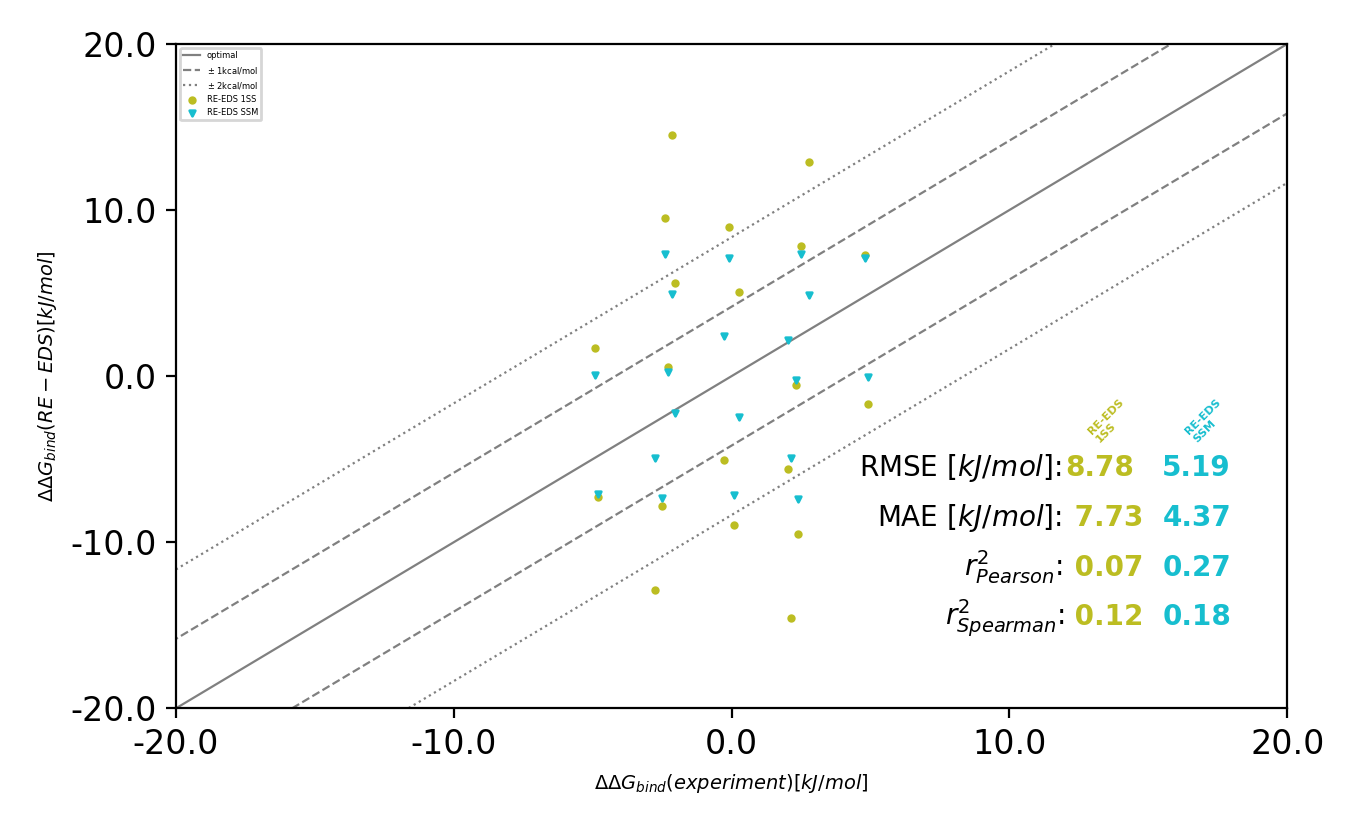
\includegraphics[width=0.8\textwidth]{fig/results/ringOpening/paramOptimization/RingClosure_system_Eoff_final_results.png}
\caption{Comparison of the relative energy offsets $\Delta \Delta E^R_{ji}$ in water and complex with the experimental relative binding free energies $\Delta \Delta G^\text{bind}_{ji}$. The energy offsets were estimated from RE-EDS simulations using the 1SS (green) or SSM (blue) approach to select the starting configurations of the replicas.} \label{SIfig:Eoff_experiment_corr_RingOpening}
\end{figure}


\subsection{Optimization of the $s$-Distribution and the energy offsets}
\begin{figure}[h]
\centering
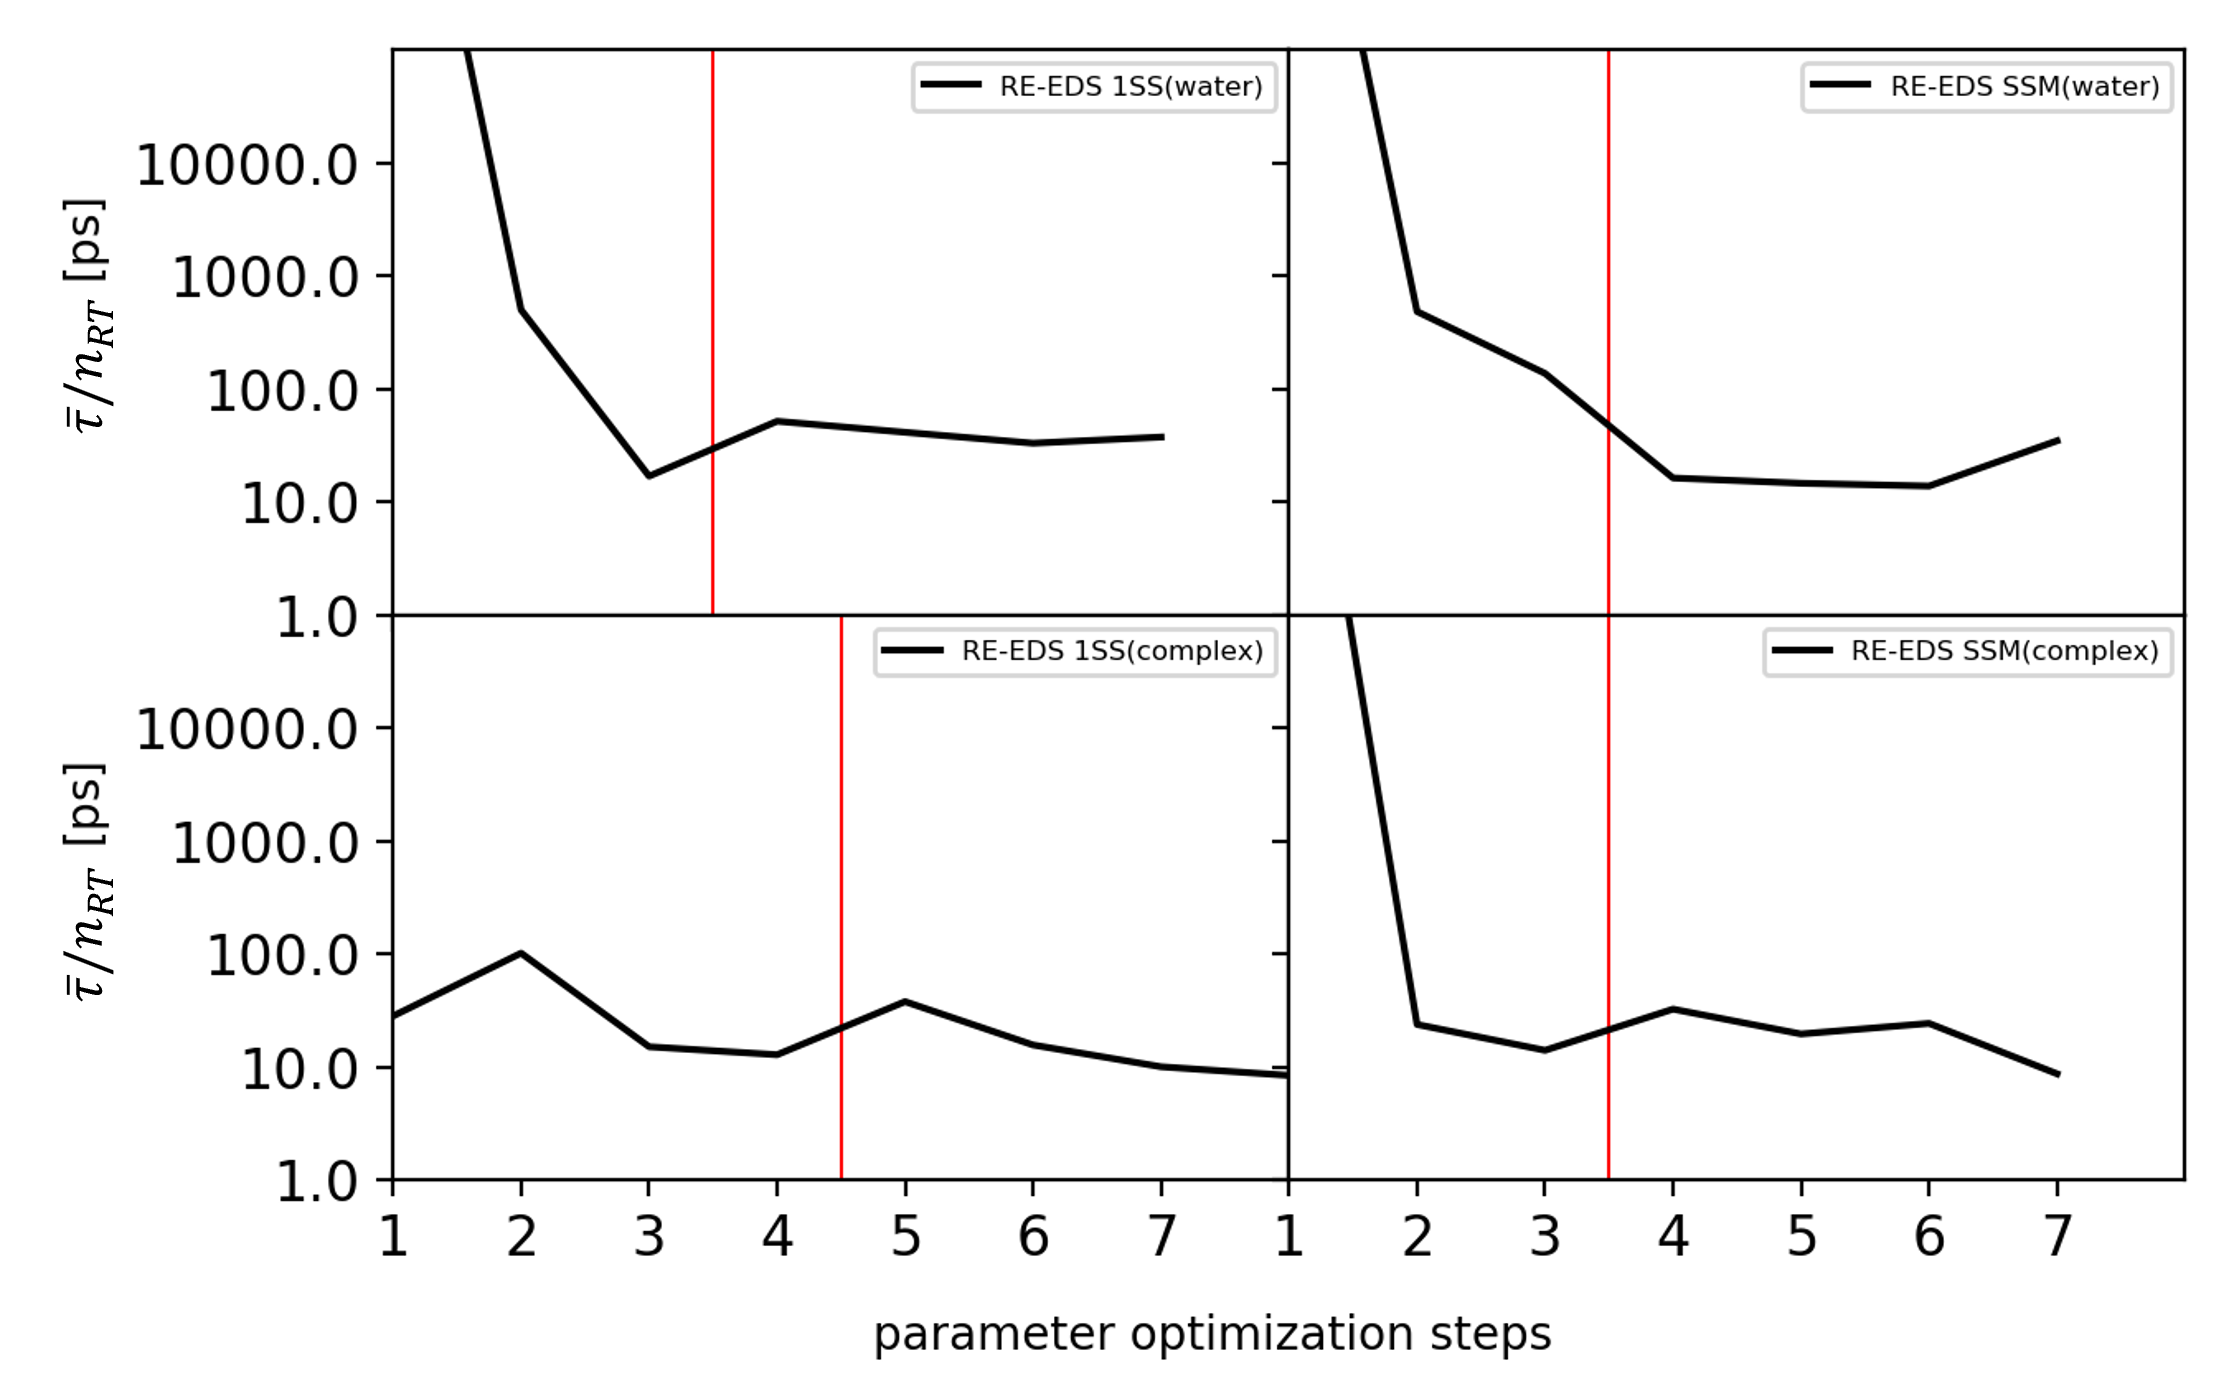
\includegraphics[width=\linewidth]{fig/results/ringOpening/paramOptimization/RingOpening_optimization_RTstat.png}
\caption{Average round-trip time as a function of the optimization steps $i$ ($\overline{\tau}_i$) on a logarithmic scale. The red line indicates the switch from $s$-optimization to energy offset rebalancing.}
\label{SIfig:CHK1_RingOpening_soptimization_efficiency}
\end{figure}

\begin{figure}[H]
\centering
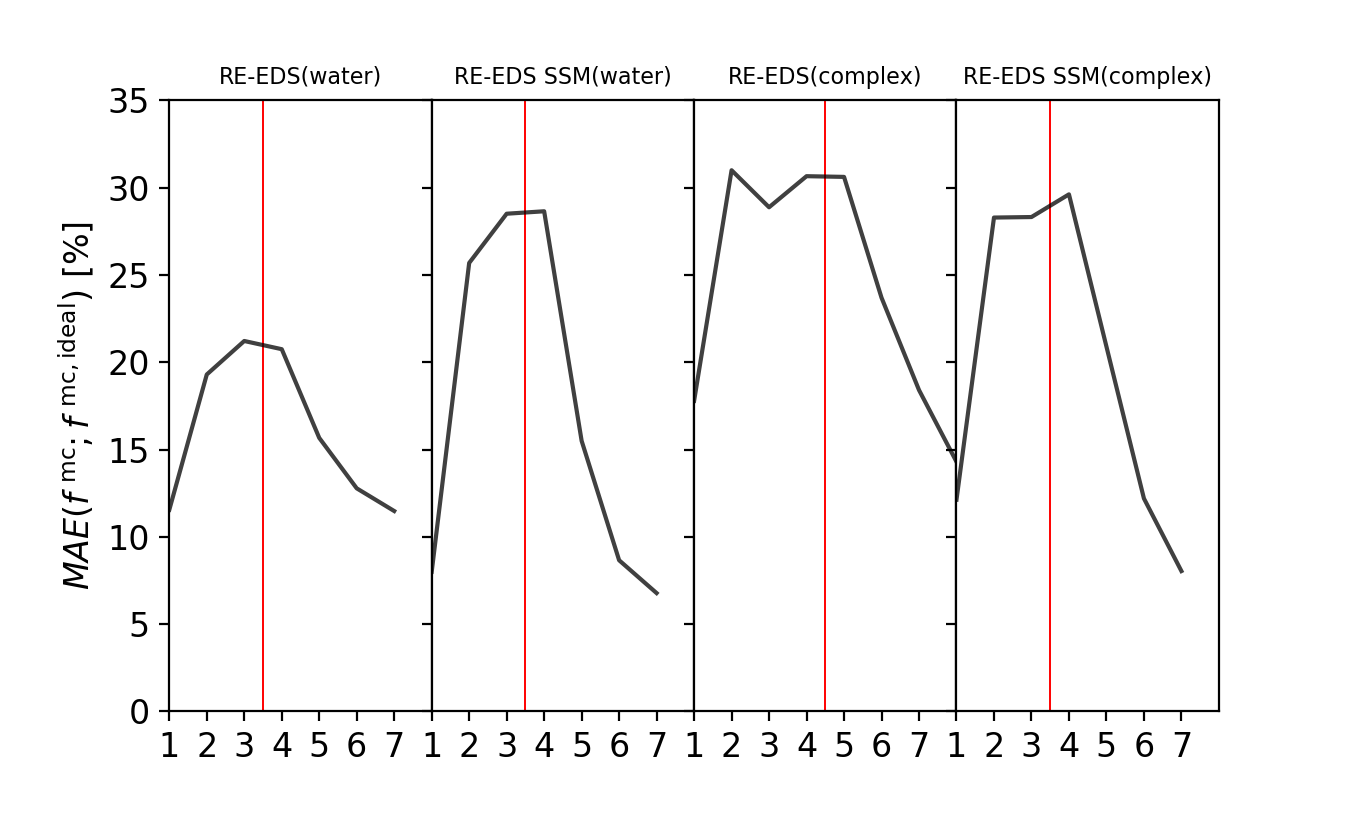
\includegraphics[width=\linewidth]{fig/results/ringOpening/paramOptimization/RingOpening_optimization_fractOptSampMAE.png}
\caption{Mean absolute deviation (MAE, in percentage) of the observed state sampling $f_i^{\text{mc}}$ from the ideal equal distribution $f_i^{\text{mc,ideal}}$ during the short optimization simulations. The red line indicates the switch from $s$-optimization to energy offset rebalancing.}
\label{SIfig:CHK1_RingOpening_optimization_fractOptSampMAE}
\end{figure}


\subsection{Free-Energy Calculation}
\begin{table}[H]
\caption{Free-energy differences in water and in complex calculated from the production run of 3.5~ns of length with the RE-EDS 1SS and RE-EDS SSM approaches.}
\begin{center}
\begin{tabular}{ c c |c c |c c}
  \multicolumn{2}{c|}{Ligand} & \multicolumn{2}{c|}{RE-EDS 1SS} &\multicolumn{2}{c}{RE-EDS SSM}\\ 
  J & I  & water [kJ~mol$^{-1}$] & complex [kJ~mol$^{-1}$]  & water [kJ~mol$^{-1}$] & complex [kJ~mol$^{-1}$] \\
  \hline
        L17 &         L1 &       11.9 $\pm$ 0.0&        17.0 $\pm$ 0.8&   12.4 $\pm$ 0.5&   9.4 $\pm$ 1.9\\
        L19 &         L1 &        2.7 $\pm$ 0.0&        5.7 $\pm$ 1.0&     3.1 $\pm$ 0.0&   8.0 $\pm$ 0.0\\
        L20 &         L1 &      -47.8 $\pm$ 0.0&      -47.6 $\pm$ 0.9& -47.7 $\pm$ 0.0&  -48.1 $\pm$ 0.0\\
        L21 &         L1 &      -61.7 $\pm$ 0.06&     -63.1 $\pm$ 0.8& -61.7 $\pm$ 0.0&  -64.8 $\pm$ 0.0\\
        L19 &         L17 &      -9.2 $\pm$ 0.0&      -11.3 $\pm$ 0.6&  -9.3 $\pm$ 0.5&   -1.4 $\pm$ 1.9\\
        L20 &         L17 &     -59.6 $\pm$ 0.0&      -64.5 $\pm$ 0.1& -60.1 $\pm$ 0.5&  -57.6 $\pm$ 1.9\\
        L21 &         L17 &     -73.6 $\pm$ 0.0&      -80.1 $\pm$ 0.1& -74.1 $\pm$ 0.5&  -74.3 $\pm$ 1.9\\
        L20 &         L19 &     -50.5 $\pm$ 0.0&      -53.2 $\pm$ 0.6& -50.7 $\pm$ 0.0&  -56.2 $\pm$ 0.0\\
        L21 &         L19 &     -64.4 $\pm$ 0.0&      -68.8 $\pm$ 0.6& -64.7 $\pm$ 0.0&  -72.9 $\pm$ 0.0\\
        L21 &         L20 &     -13.9 $\pm$ 0.0&      -15.5 $\pm$ 0.2& -14.0 $\pm$ 0.08& -16.7 $\pm$ 0.0 \\
\end{tabular}
\end{center}
\label{SItab: RE-EDS_FE_RingCycleOpening_dFs}
\end{table}

\begin{figure}[H]
\centering
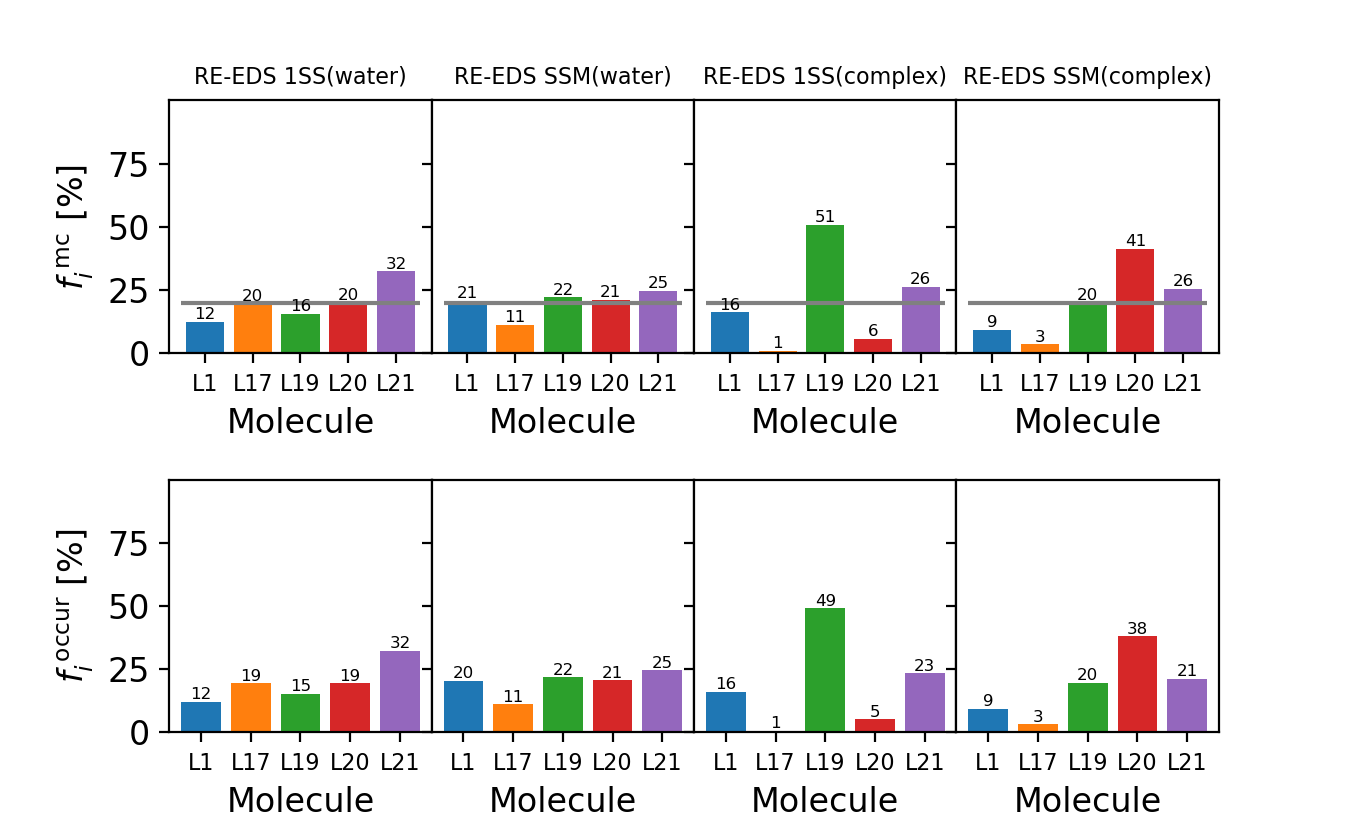
\includegraphics[width=\linewidth]{fig/results/ringOpening/FE/Reeds_RingOpening_production_sampling_s1.png}
\caption{Sampling of the end states in the final production run at replica $s=1.0$. Sampling was assessed by monitoring the maximally contributing end state (top panels) and by counting all end states a potential energy below $T_{i}^{phys}$ (see Table \ref{SItab:RingCycleOpenin_PotentialTresholds}) (bottom panels). Ideally, the sampling fraction as maximally contributing end state should be 1/$N$ (Eq. (8) in the main text) for all end states, indicated as a black horizontal line.}
\label{SIfig:CHK1_RingOpening_soptimization_final_Sampling_s1}
\end{figure}


\begin{figure}[H]
\centering
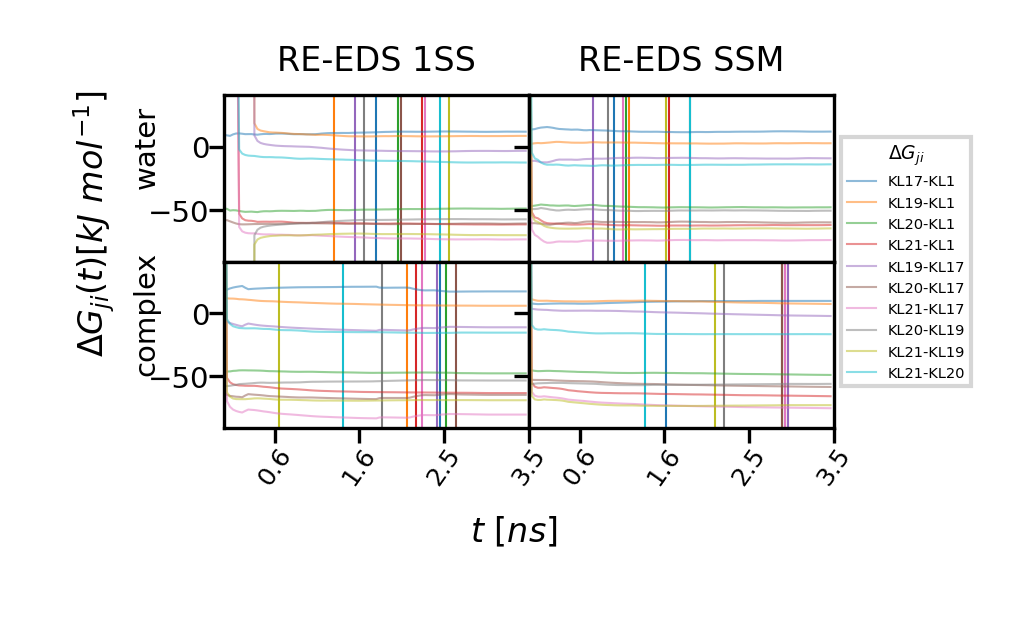
\includegraphics[width=\linewidth]{fig/results/ringOpening/FE/dF_RingOpening_Convergence.png}
\caption{Convergence analysis of the RE-EDS production runs (total 3.5~ns): The free-energy results are plotted as a function of the simulation time. The vertical lines indicate when a particular $\Delta G_{ji}$ value was found to be converged (deviation below 1~kJ~mol$^{-1}$).}
\label{SIfig:CHK1_RingOpening_dF_convergence}
\end{figure}


\clearpage
\newpage

%================================================================================
\section{Conclusion}
%================================================================================

In this work, we presented an efficient algorithm for the placement of distance restraints in a linked dual topology approach that can easily be applied or incorporated into pipelines with the provided git repository and a python anaconda environment \cite{anaconda} \textit{\hyperlink{https://github.com/rinikerlab/restraintmaker}{https://github.com/rinikerlab/restraintmaker}}. The algorithm can be used in python scripts or interactively with a representation of the molecules in PyMol 2.0 (or higher). Distance restraint files can be written in GROMOS and GROMACS format, or in an easily accessible and human-readable JSON format that can be parsed by any JSON parser. \cite{DeLano2020}

The presented algorithm is a graph-based approach and can be straightforwardly applied to molecules with a rigid core. With this, the only required user input is the number of restraints assigned to link two molecules.

%%%%%ToyModelFun
The introduced algorithm was tested, and its time and result performance were analyzed with toy models and compared to brute force approaches. This test found that the algorithm represents a good trade-off between time and algorithmic complexity compared to the brute force approaches.

%%%%%TI
Relative hydration free energy calculations were presented for pairwise TI approaches, showing the influence of the restraints on the convergence of the simulations, and the sampling behavior of molecules containing a rigid core, like commonly used in pharmaceutical drug discovery, is minimal.

%%%%%%REEDS
For multistate methods, we expanded our scheme in order to match the requirements of such approaches. It could be shown that the relative hydration free energies obtained with RE-EDS results in a similar accuracy as the pairwise TI calculations, but using a shorter simulation time.

As an outlook, we would like to point out that our future work on multistate methods will be expanding on this work, and we are looking forward to using the approach for more complex systems. Interesting challenges include increasing the number of states significantly or going to larger molecules.

\clearpage
\pagebreak

%================================================================================
%\section{Appendix}
%================================================================================
\begin{ethappendix}
%================================================================================
\appsection[CBTI and Quadrature]{quad}{Relationship between CBTI and Quadrature Integration}
%================================================================================
This appendix investigates the convergence properties of the CBTI scheme upon
increasing the number $K$ of replicas based on an analogy with quadrature integration. More precisely, it is  shown that the 
\radd{variation amplitude} $G_{\Lamb}^\star$ \radd{of $G_{\Lamb}(\Lamb)$} decreases at least as $K^{-1}$ \radd{in the limit of large $K$}
%upon increasing $K$ 
%\radd{for large $K$}
(with $K$ even), as suggested by \reffig{scheme:ldyn:gotoflat} and \reff{deltag}.


To this purpose, we first observe that the situation of a conveyor belt (CB) spanning the $\lam$-range $[0,1]$ of the free-energy profile $G(\lam)$ with $K$ equidistant replicas at \radd{spacings $2K^{-1}$} along the cable (\reffig{train:cvb}) is mathematically equivalent to the situation of a train spanning a periodic function $g(x)$ of period $2\pi$ with $K$ equidistant carriages at \radd{spacings $2\pi K^{-1}$} spanning one period (\reffig{train:gx}).
%
The function $g(x)$ is obtained by mirroring $G(\lam)$ \radd{at $\lam=0$ or $1$}, periodically translating the mirrored function by integer multiples of two, and stretching $\lam$ by a factor of $\pi$ to define the new variable $x$.

\begin{figure}[H]
  \centering
  \subgraph{fig:train:cvb}{conveyor_belt_sintw_without_arrows.pgf}{.5}\\
%  \subgraph{fig:train:train}{train_sintw.pgf}{1.0}\\
  \subgraph{fig:train:gx}{app_gx.pgf}{.99}%
  \caption{\footnotesize\captitital{Analogy between the CBTI scheme and the sampling of an even
    periodic function by a train of equispaced points.}
    The illustration considers a conveyor belt (CB) with $K=8$ replicas, analog
  to a train with 8 carriages.}
  \label{fig:train}
\end{figure}


In this analogy, we now have a periodic function $g(x)$ of period $2\pi$ that is even over the reference interval $[0,2\pi)$.
%
    This function is sampled by $K$ equidistant points at locations

    \beq{xm}
    x_k = s+kh\quad\text{with}\quad k=0 \dots K-1\quad\text{and}\quad h=2\pi K^{-1},
    \eeq
%
    where $s$ represents the offset position of the first point $k=0$.
%
    Note that $s$ can always be selected in the interval $[0,h)$ 
    by consideration of periodicity, along with an appropriate renumbering of the points carriages. 
We also introduce the negative first derivative of the function

        \beq{fx}
        f(x)=-g'(x).
        \eeq

In practical applications of CBTI, the Hamiltonian-coupling scheme 
will 
%generally 
be defined by a continuously differentiable function of $\lam$, in which case $G(\lam)$ is also continuously differentiable. The same applies to $g(x)$ in the analogy of \reffig{train:gx}, except for the possible occurrence of kinks at integer multiples of $\pi$. These occur because the derivative $G'(\lam)$ of $G(\lam)$ generally differs from zero at the physical end-states $\lam=0$ or $\lam=1$. As a result, $f(x)$ is continuous except at these points, where it will present jumps. An illustrative example for functions $g(x)$ and $f(x)$ with the above properties is shown in \reffigs{app:g} and \reff{app:f}, respectively.

In the analogy of \reffig{train:gx} to the CB situation, the total force on the \radd{train of points} (analog to the mean force on the $\Lamb$-variable) is given for a specific value of $s$ (analog to the $\tilde{\Lamb}$-variable) by 
%
\beq{total_force}
F(s) = \sum\limits_{k=0}^{K-1}f(kh+s).
\eeq
%
As illustrated in \reffig{app:ftrapz}, this sum has a simple interpretation. It represents a trapezoidal quadrature
estimate to the integral of the periodic function $f(x)$ over the period $[s,2\pi+s)$. Because $f(x)$ is the negative derivative of the periodic function $g(x)$, its exact integral over one period must be zero. Thus, \radd{for any $s$,} we expect $F(s)$ to converge to zero in the limit $K\rightarrow \infty$. The following paragraphs investigate the corresponding convergence rate.
%
 
\begin{figure}[H]
  \centering
  \subgraph{fig:app:g}{gx_ene_ana.pgf}{.49}%
  \subgraph{fig:app:f}{fx_ene_ana.pgf}{.49}\\
  \vspace{-1em}%
  \subgraph{fig:app:ftrapz}{fx_trapz_ene_ana.pgf}{.49}\\
  \vspace{-1em}%
  \subgraph{fig:app:tildeF}{tildeF_ene_ana.pgf}{0.49}%
  \subgraph{fig:app:tildeG}{tildeG_ene_ana.pgf}{0.49}\\
  \vspace{-1em}%
  \subgraph{fig:app:Rs}{Rs_ene_ana.pgf}{0.49}%
  \subgraph{fig:app:Rprimes}{Rprimes_ene_ana.pgf}{0.49}\\
  \caption{\footnotesize\captitital{Illustrative functions supporting the discussion in \refsec{quad}.}
    Panel (\subref{fig:app:g}) shows the illustrative function $g(x)$ defined 
    over the reference period $[0;2\pi[$ as 
        $x+\sin (x^2)$ if  $x<\pi$ or 
        $(2\pi-x)+\sin ((2\pi-x)^2)$ if $x\geq\pi$.
    %
    Panel (\subref{fig:app:f}) shows the negative derivative $f(x)$ of $g(x)$.
    %
    Panel (\subref{fig:app:ftrapz}) illustrates the trapezoidal integration of $f(x)$ (blue)
    as a shaded area (orange) with $K=8$ and $s=0.4$. The vertical lines show the positions of the
    carriages at values $x_m$. The trapezoids are seen to represent a poor approximation
    at the discontinuities.
    %
    Panel (\subref{fig:app:tildeF}) illustrates the total force $\tilde{F}(\tilde{s})$ 
    of \refeq{total_force_tilde} for different values of $K$.
    %
    Panel (\subref{fig:app:tildeG}) illustrates the potential energy $\tilde{G}(\tilde{s})$
    for different values of $K$.    which is the running integral of $\tilde{F}$ for different numbers of replicas $K$.
    %
    Panel (\subref{fig:app:Rs}) shows in a log-log form the residual integral 
    $R(\tilde{s})$ of \refeq{r_of_s} 
    as a function of $K$ for different values of $\tilde{s}$. 
    %
    Panel (\subref{fig:app:Rprimes}) shows in a log-log form the corrected residual integral  $R'(\tilde{s})$ of \refeq{r_prime_of_s_tilde}. Note that the logarithm of the absolute value of $R$ or $R'$ is displayed. The cusp in Panel (\subref{fig:app:Rprimes}) is explained by a change of sign.
  %% Bottom left: $log(\tilde{I})$ vs $\log(M)$. The dashed lines denote fits. The slope is always 
  %% -1.
  %% Bottom right: $log(\tilde{F})$ (net force) vs. $\log(M)$
  }
  \label{fig:app}
\end{figure}

     
%
The function $F(s)$ is periodic of period $h$, odd over the reference interval $[0,h)$
and generally discontinuous at $s$ values which are integer multiples of $h$.
%
Introducing  
%
\beq{total_force_tilde}
\tilde{s}=h^{-1}s \quad\text{and}\quad\tilde{F}(\tilde{s}) = F(h\tilde{s})=\sum\limits_{k=0}^{K-1}f((k+\tilde{s})h),
\eeq
%
the function $\tilde{F}(\tilde{s})$ is periodic of period 1, odd over the reference interval $[0,1)$ and generally discontinuous at integer values of $\tilde{s}$.

The corresponding potential energy of the \radd{train of points} (analog to the free-energy profile $G_{\Lamb}(\Lamb)$ of the CB 
%scheme 
over the \radd{interval $[0,2\pi K^{-1}]$}) is given by
%
\beq{train_energy}
G(s)=-\int\limits_{0}^{s} \mathrm{d}s' F(s').
\eeq
%
The function $G(s)$ is periodic of period $h$, even over the reference
interval $[0,h)$ with an extremum at $h/2$, and possibly presents kinks at $s$ values which are integer multiples of $h$.
%
Using the variable $\tilde{s}$ and introducing
%
\beq{train_energy_tilde}
\tilde{G}(\tilde{s})=-\int\limits_{0}^{\tilde{s}} \mathrm{d}\tilde{s}' \tilde{F}(\tilde{s}') \ ,
\eeq
%
one may write
%
\beq{train_energy_to_tilde}
G(s) = h \tilde{G}(h^{-1}s).
\eeq
%
The function $\tilde{G}(\tilde{s})$ is periodic of period 1, even over
the reference interval $[0,1)$ with an extremum at $1/2$,
and possibly presents kinks at integer values of $\tilde{s}$.

The functions $\tilde{F}(\tilde{s})$ and $\tilde{G}(\tilde{s})$
corresponding to the illustrative functions $g(x)$ and $f(x)$ are shown in \reffigs{app:tildeF} and \reff{app:tildeG}, respectively, considering the choices $K=2,4,8,16,32$ or $64$.
%
Convergence is observed upon increasing $K$,
%(decreasing $h$), 
in which
% case 
$\tilde{F}(\tilde{s})$
becomes linear and $\tilde{G}(\tilde{s})$ parabolic over the reference interval
$[0,1)$. Thus, \radd{in the limit of large $K$}, one expects the maximal variation $\tilde{G}^\star$ in $\tilde{G}(\tilde{s})$
to converge to a constant and, \textit{via} \refeq{train_energy_to_tilde}, the maximal variation $G^\star$
in $G(s)$  (analog to the corresponding maximal variation $G_{\Lamb}^\star$ of  $G_{\Lamb}(\Lamb)$ in the CB scheme)
to \radd{scale as $h$, {\em i.e.} as $K^{-1}$}.

This observation, made here in a special case, can be generalized as follows.
%
Given
%
\beq{r_of_s}
R(\tilde{s})=h\tilde{F}(\tilde{s}) = h\sum\limits_{k=0}^{K-1}f(h(k+\tilde{s})),
\eeq
%
$G^\star$ is the absolute extremum (largest absolute value) of the function
%
\beq{s_of_s}
S(\tilde{s})=h\tilde{G}(\tilde{s}) = \int\limits_{0}^{\tilde{s}} \mathrm{d}\tilde{s}' R(\tilde{s}')
\eeq
%
over the $\tilde{s}$-interval $[0,1/2]$.
%
According to \reffig{app:ftrapz}, the quantity $R(\tilde{s})$ is the residual of the trapezoidal quadrature approximation to the integral of $f(x)$ over one period, where the first grid point is offset from the origin by a fraction $\tilde{s}$ of the spacing $h$. 
%
If $f(x)$ was continuous everywhere, the convergence would be quadratic in $h$ (\ie{} scale as $K^{-2}$), as expected from a trapezoidal quadrature. However, the presence of discontinuities in $f(x)$ at $0$ and $\pi$ introduces an error that is linear in $h$.
%
To recover quadratic convergence, one would need to introduce a correcting term for the points $0,K/2-1,K/2$ and $K-1$ surrounding the discontinuities, namely

\begin{align}
\label{eq:r_prime_of_s_tilde}
R'(\tilde{s})=&R(\tilde{s}) + h 
   \bigg\{
    \frac{\tilde{s} - 1}{2} 
    \left  [
      f(h\tilde{s}) + f\left (h\left(\tilde{s}+\frac{K}{2}\right)\right)
    \right ] \nonumber \\
    &- 
     \frac{\tilde{s}}{2} 
    \left  [
      f(h(\tilde{s}+K-1)) + f\left(h\left(\tilde{s}+\frac{K}{2}-1\right)\right)
    \right ] \nonumber \\
    & + \left(\tilde{s} -\frac{1}{2}\right)
    \left ( 
      \Delta_0 + \Delta_\pi
    \right )
  \bigg \}
\end{align}
%
where $\Delta_0$ and $\Delta_\pi$ account for the magnitude of the discontinuities, \ie

\beq{discont}
\Delta_0=\lim_{x\xrightarrow{>} 0}f(x)\quad\text{and}\quad\Delta_\pi=\lim_{x\xrightarrow{>} \pi}f(x).
\eeq

The convergence of $R(\tilde{s})$ and $R'(\tilde{s})$ for the illustrative functions
$g(x)$ and $f(x)$ upon increasing $K$ along with the choices $\tilde{s}=0.01, 0.2, 0.3, 0.4,0.49$ 
is shown in  logarithmic form in \reffigs{app:Rs} and \reff{app:Rprimes}, respectively.
%
As expected, for large $K$, $R$ shows a linear convergence (slope -1) and $R'$
a quadratic one (slope -2). 
%
The limiting cases $\tilde{s}=0$ and $\tilde{s}=1/2$ are special. For $\tilde{s}=0$, \refeq{r_of_s}
implies an evaluation of $f(x)$ at the discontinuity. If one uses an average value of $0$ for these points, $R(0)$ evaluates to 0 for any $K$ by symmetry. 
%Similarly, for $\tilde{s}=1/2$, $R(1/2)$ evaluates to 0 for any $K$ by symmetry. 
\radd{The same applies for $\tilde{s}=1/2$, $R(1/2)$.}
For all other values for $\tilde{s}$, the convergence is as expected, \ie{} linear for $R(\tilde{s})$ and quadratic for $R'(\tilde{s})$.

If $R(\tilde{s})$ converges to zero as $K^{-1}$ for (nearly) all $\tilde{s}$ values,
the function $S(\tilde{s})$ of \refeq{s_of_s} will converge to zero with the same scaling, and so will its absolute extremum $G^\star$. We conclude that the magnitude \radd{$G^\star_{\Lamb}$} of the residual variations
in $G_{\Lamb}(\Lamb)$ for the CBTI scheme scales at least as $K^{-1}$ \radd{in the limit of large $K$}. And if $G(\lam)$ has a vanishing derivative at the physical end-states, it will scale at least as $K^{-2}$.
%
It should be stressed, however, that these are worst-case scalings. A higher level of continuity or specific symmetry properties of $G(\lam)$ may tighten the scaling. 
%
To give an extreme case, for a free-energy profile $G(\lam)=\cos (2\pi\lam)$,
one shows easily that the residual variations \radd{$G^\star_{\Lamb}$} entirely vanish irrespective of $K$. 
%
This follows from 
\beq{cos}
\sum\limits_{k=0}^{K-1}\cos \left (2\pi K^{-1}k + c \right ) = 0\quad\forall~c \quad \text{(for }K\text{ even)}.
\eeq

The present analysis connects the convergence of the CBTI scheme with $K$ to the properties of a quadrature integration. This connection opens interesting tracks for future work. In particular, it suggests that these convergence properties could be improved by altering the coupling scheme (\eg{} to enforce vanishing $G(\lam)$ derivatives at the end-states), the function $\zeta$ in \refeq{cb_lam_of_big_lam} (\eg{} higher system density close to discontinuities) and the CBTI weighting in \refeq{ti_rep_ham} (\eg{} from trapezoidal to higher-level quadrature, \eg{} Simpson or even Romberg).


%================================================================================
\appsection[CBTI Parameters]{othersim}{Choice of the CBTI Parameters}
%================================================================================
Here, we explore the influence of the CBTI 
mass parameter $m_\Lambda$ and thermostat coupling 
time $\tau_\Lambda$ considering different numbers $K$ 
of replicas. 
%

A first set of simulations involves the choices $m_{\Lambda}=$16, 160, 800, 1600 or 3200$\,\mathrm{u}\,\mathrm{nm}^2$,
      along with $K=16$ replicas in the absence of separate thermostat coupling 
      for $\Lambda$, {\em i.e.} $\tau_\Lambda\rightarrow\infty$
      (10 ns simulations after $0.2\unit{ns}$ equilibration).
%
The results are shown graphically in \reffigs{thermo:03_cvb_screen:016:1_0.01} - \reffign{thermo:03_cvb_screen:016:200_0.01} and reported numerically in \reftab{screen} (entries 1-5).
%
In the absence of explicit
%specific 
thermostating for the $\Lamb$-variable, the average
temperature $T_{\Lamb}$ of this variable is controlled exclusively by its 
coupling to the conformational degrees of freedom, 
themselves thermostated by the application of SD with a reference temperature of $298.15\unit{K}$
and an effective coupling time of $0.1\unit{ps}$.
%
All choices of $m_{\Lamb}$ considered lead to average temperatures $T_\Lamb$
close to $298.15\unit{K}$, suggesting an appropriate kinetic-energy exchange.
 The mass-parameter
choices of  $m_\Lamb=16\,\mathrm{u\,nm^2}$ 
and $1600\,\mathrm{u\,nm^2}$ present the largest deviations of about $10\unit{K}$ and $6\unit{K}$,
respectively, while the deviation is at most $2\unit{K}$ for the other choices.


Expectedly, increasing $m_{\Lamb}$ tendentially leads to a decrease in the
diffusion coefficient $D_\Lambda$.
%
This results from a smaller width $\sigma_{\dot{\Lamb}}$ of the $\dot{\Lamb}$ distribution 
(\refeq{ana_vel}; see also \reffig{dynamics:vel} where $m_{\Lamb}$ increases from left to right),
\ie{} a lower average magnitude of the velocity along $\Lamb$. 
However, $D_{\Lamb}$ is also affected by the presence of residual variations 
in the free-energy profile $G_{\Lamb}(\Lamb)$, which may be more easily overcome at higher $m_{\Lamb}$
(more inertia). This is reflected in the increase of the $\dot{\Lamb}$ autocorrelation time $\tau_{\dot{\Lamb}}$ upon increasing $m_{\Lamb}$ (see also \reffig{acf} for the corresponding \radd{normalized} autocorrelation functions). This second effect is likely to have more influence for \radd{small $K$},
where the $G_{\Lamb}(\Lamb)$ variations are more pronounced. 
In the present case with $K=16$, these opposite effects probably 
explain why the trend in $D_{\Lamb}$ upon increasing $m_{\Lamb}$ is not strictly
monotonic, with a comparatively high $D_{\Lamb}$ for 
$m_{\Lamb}=1600\unit{u\,nm^2}$ (see also \reffig{dynamics:dif} where the diffusion trend is non-monotonic
upon increasing $K$ when  $m_{\Lamb}$ is made proportional to $K^{1/2}$).



In terms of the calculated free-energy change $\Delta G$, all simulations provide the same 
values within the statistical error, with a slightly larger deviation for the simulation 
involving the lowest mass $m_{\Lambda}=16\unit{u\,nm^2}$, probably due to the comparatively large $T_{\Lamb}$ deviation.
%
Because it leads to accurate $T_{\Lamb}$ and $\Delta G$ values while presenting a high $D_{\Lamb}$,
the second-to-lowest mass $m_\Lamb=160\,\mathrm{u\,nm^2}$ was chosen for all 
following CBTI simulations employing $K=16$ replicas. 


A second set of simulations involves a separate coupling of the $\Lamb$ variable to a 
Nos\'e-Hoover chain thermostat with the
choices $\tau_\Lambda=$0.05,0.1,0.5,1 or 2$\,\mathrm{ps}$
along with $K=16$ replicas and $m_{\Lambda}=160\,\mathrm{u}\,\mathrm{nm}^2$
($10\unit{ns}$ simulations after $0.2\unit{ns}$ equilibration).
%
The results are shown graphically in \reffigs{thermo:02_cvb_thermo_screen:016:10_0.05} - 
\reffign{thermo:02_cvb_thermo_screen:016:10_2.0} and reported numerically in \reftab{screen} (entries 6-10).
%
Except for the two shortest coupling times,
the average temperature $T_\Lambda$ is very close to the reference temperature, with a maximal
deviation of about $2\unit{K}$. The larger deviations for $\tau_{\Lamb}=0.05$ or $0.1\unit{ps}$ suggest that the coupling of $\Lamb$ to its thermostat should be made less tight than that of the conformational degrees of freedom to their thermostat (here SD with $0.1\unit{ps}$). The coupling parameter $\tau_{\Lamb}$ has no
influence on the width $\sigma_{\dot{\Lamb}}$ of the $\dot{\Lamb}$ distribution,  which is the
same for all five simulations and very close to the Maxwell-Boltzmann one (\refeq{ana_vel}). 
On the other hand, a lower $\tau_{\Lamb}$, \ie{} a tighter coupling, reduces the
inertia of the conveyor belt, which results in a decrease of the autocorrelation time $\tau_{\dot{\Lamb}}$. This leads to a tendential decrease of $D_{\Lamb}$ upon decreasing $\tau_{\Lamb}$.
%
In terms of the calculated $\Delta G$, all simulations provide consistent values within the statistical error, with a slightly larger deviation for the simulation involving $\tau_{\Lamb}=0.05\unit{ps}$, probably again due to the comparatively large $T_{\Lamb}$ deviation. 
%
In comparison to the first set of simulations with $\tau_{\Lamb}\rightarrow \infty$, the $\Delta G$ values are slightly higher ($0.1-0.3\unit{kJ\,mol^{-1}}$), which could be due to the fact that the sampled $\dot{\Lamb}$ distribution $P_{\dot{\Lamb}}$ is even closer to the Maxwell-Boltzmann distribution (\refeq{ana_vel}), also for shorter time intervals.
%
For $\tau_{\Lamb}\geq 0.5\unit{ps}$, the choice of $\tau_{\Lamb}$ has little influence on the calculation, and a coupling time $\tau_{\Lamb}=0.5\,\mathrm{ps}$
was chosen for all following CBTI simulations. Note, however, that a looser coupling could be of advantage by leading to a higher $D_{\Lamb}$.


A third set of simulations considers the choices $K=$8, 16, 32, 64 or 128
along with 
$m_{\Lamb}=40 K^{1/2}\,\mathrm{u}\,\mathrm{nm}^2$
and $\tau_{\Lamb}=0.5\,\mathrm{ps}$ 
($256 K^{-1}\unit{ns}$ simulations after $0.2\unit{ns}$ equilibration). 
%
The results are shown graphically in \reffigs{thermo:04_cvb_thermo:008:10} - \reffign{thermo:04_cvb_thermo:128:10} and reported in \reftab{screen} (entries 11-15).
%
Simulations 11, 13 and 15 are discussed in details in \refsec{results} (see \reffigs{lam} and \reff{dynamics}).
%
For the five simulations, the average temperature $T_{\Lamb}$ is close to the target temperature,
with a maximal deviation of about $6\unit{K}$.
%
The free-energy differences $\Delta G$ are consistent within
the statistical error, except for the simulation employing $K=8$ replicas (entry 11),
which is due to the non-uniform sampling of the $\lam$-range as discussed in \refsec{results}.
%

The rationale for making the mass $m_{\Lamb}$ proportional to the square-root of $K$, \revphil{an arbitrary parameter choice,} is the following. 
If one wishes the CB variable $\Lamb$ to evolve dynamically on comparable timescales irrespective of the number $K$ of replicas attached to it, one should ensure that its acceleration $\ddot{\Lamb}$
depends only weakly on $K$. Assuming that the forces exerted by the $K$ replicas are essentially uncorrelated, their sum (\ie{} the net force on the CB) will scale as $K^{1/2}$. 
Thus, an identical scaling of $m_{\Lamb}$ is required to preserve an approximately constant $\ddot{\Lamb}$. The time series and distributions of $\ddot{\Lamb}$ for different choices of $K$ when using this scaling for $m_{\Lamb}$ (see \reffig{dynamics:acc}) are indeed similar, 
supporting the above considerations.
%this choice for the $m_{\Lamb}$ scaling.

In summary, this appendix shows that when selected within reasonable ranges,
the parameters $m_\Lambda$ and $\tau_\Lambda$ have only a limited 
influence on the kinetic-energy exchange between $\Lambda$ and the conformational
degrees of freedom, on the temperature $T_\Lambda$, on the diffusion constant $D_\Lamb$, 
and on the calculated free energies $\Delta G$.
%
In \refsec{results}, \revphil{working} choice
$m_{\Lamb}=40 K^{1/2}\,\mathrm{u}\,\mathrm{nm}^2$ 
and $\tau_{\Lamb}=0.5\,\mathrm{ps}$ 
is selected for all CBTI calculations.


\revphil{
%================================================================================
\appsection[Simplified Estimators]{CH2C}{\revphil{Simplified Free-energy Estimators}}
%================================================================================
}



%
%
The free-energy estimator employed here for CBTI is
given by \refeq{cbti_formula}.
%
The approximation involved corresponds to a 
simple forward rectangular quadrature, where the Hamiltonian derivative is 
averaged over $J$ successive bins considering all replicas simultaneously.
%
%Since $\tilde{P}(\tilde{\Lamb})$ and thus $p(\lam)$ are typically close to homogeneous, $J$ can be taken very large, resulting in a negligible quadrature error. For example, 
%
If $K$ replicas sample $L$ configurations each, and $p(\lam)$ is close to homogeneous,
the number of data points per bin will be close to $K L/J$, with limited variations across bins. 
%We define the maximal allowed value $J_{\mathrm{max}}$ as the highest value of $J$ for which empty bins 
%(vanishing denominator in the ensemble average of \refeq{cbti_formula}) never occur. 
%In practice, a graph of $\Delta G$ evaluated upon increasing $J$ from 1 to $J_{\mathrm{max}}$ will 
%rapidly level off to a plateau when quadrature errors become sufficiently small. 
%
In this case, one may consider a simpler alternative to \refeq{cbti_formula} that does 
not involve the specification of a number of bins.
%


Considering all the $K$ replicas simultaneously,
the $KL$ pairs of $\lam$-values and associated Hamiltonian 
derivatives are sorted in ascending order for $\lam$ (index $i=0,...,KL-1$),
One then calculates
%
\beq{cbti_formula_app1}
\Delta G_{\mathrm{alt}}=(KL)^{-1}\sum\limits_{i=0}^{KL-1} \frac{\lam_{i+1}-\lam_{i-1}}{2} \left ( \frac{\partial \ham}{\partial \lam}\right )_{i}
\eeq
%
using $\lam_{-1}=\lam_{KL}=0$.
%
This alternative estimate, noted $\Delta G_{\mathrm{alt}}$, considers that each sample $i$ defines 
its own single-point bin, of width determined by contact to the next lower and higher 
data points $i-1$ and $i+1$, respectively, thereby accounting for a possible heterogeneity in the $\lambda$-sampling.
%


In the limit where the sampling becomes sufficiently close to homogeneous, 
\refeqs{cbti_formula} or \refeqn{cbti_formula_app1} can be replaced by an even simpler 
approximate expression, namely 
%
\beq{cbti_formula_average}
  \Delta G_{\mathrm{app}} \approx K^{-1} \sum_{k=0}^{K-1} \left \langle \frac{\partial \ham(\xv_k;\lam_k)}{\partial \lam_k}  \right \rangle ^{\dagger \star} ,
\eeq
%
which corresponds to averaging the Hamiltonian derivative over all replicas and over the entire CBTI simulation. 
This approximate estimate, noted $\Delta G_{\mathrm{app}}$, assumes that the $KL$ data points are on average equispaced along $\lam$, 
which only holds in the limit of homogeneous sampling.
%


The accuracy
of the estimate $\Delta G$ of \refeq{cbti_formula} with $J=500$ (except for entry 11, $J = 200$)
is compared in \reftab{screen}
to those of the simpler expressions $\Delta G_{\mathrm{alt}}$ and $\Delta G_{\mathrm{app}}$, which do not require the specification of a number of bins.
%
%of \refeqs{cbti_formula_app1} and \refeq{cbti_formula_average}
%
%
%The estimate $\Delta G_{\mathrm{alt}}$ assumes that each sampled $\lam$-value
%is at the center of its own bin, limited on the left and on the right by contact to the bin of 
%the next lower and next higher sampled $\lambda$-value.
%
The estimate $\Delta G_{\mathrm{alt}}$ is very close to $\Delta G$ (within error bar),
suggesting that \refeq{cbti_formula_app1}, which assumes that each sampled $\lam$-value
is at the center of its own bin, is a viable parameter-free alternative to \refeq{cbti_formula}. 
%
On the other hand, the estimate $\Delta G_{\mathrm{app}}$,
which assumes that each bin encompasses the same number of sampled $\lambda$-points
irrespective of $J$, is more approximate.
%
As expected from the involved assumption, $\Delta G_{\mathrm{app}}$ is only a good approximation
to $\Delta G$ when the CBTI sampling is indeed close to uniform along $\lambda$.
%
Considering entries 11-17, this is essentially the case for the unbiased simulations with $K\ge 32$.
%
However, for the unbiased simulation with $K=8$ and the two biased simulations, 
the sampling is not sufficiently homogeneous and the discrepancy can be significant
(about $1-5\unit{kJ\, mol^{-1}}$).


%--------------------------------------------------------------------------------
\appsection[Autocorrelation]{CH2D}{Autocorrelation of the Hamiltonian Derivative}
%--------------------------------------------------------------------------------

\begin{figure}[H]
  \centering
    \input{\path/plt/tcf_all_ene_ana.pgf}%
    \caption{\footnotesize\captitital{Normalized autocorrelation function $f(t)$ of the Hamiltonian derivative for the aqueous methanol-to-dummy mutation at $298.15\unit{K}$ and $1\unit{bar}$ with the 2016H66 force field.} These functions are based on the TI calculation relying on $K_{\mathrm{TI}}=17$ $\lam$-points. The functions displayed correspond to every second $\lam$-point. The associated autocorrelation times $\tau_{f}$ are reported in \reftab{tcf}. 
      %
      %% The definition of the discrete autocorrelation function $f(t)$ with lag time $t$ is given as 
      %% $f(t)=1/\sigma_x^2 \sum\limits_{i=0}^{N-t}(x_i-\overline{x})(x_{i+t}-\overline{x})$.
}
    \label{fig:ti:tcf}
\end{figure}
\clearpage

\begin{table}[H]
  \centering
\caption{\footnotesize\captitital{Autocorrelation times $\tau_f$ of the Hamiltonian derivative for the aqueous methanol-to-dummy mutation at $298.15\unit{K}$ and $1\unit{bar}$ with the 2016H66 force field.} These times are based on the TI calculation relying on $K_{\mathrm{TI}}=17$ $\lam$-points. The associated autocorrelation functions $f(t)$ are displayed in \reffig{ti:tcf} for every second $\lam$-point. The autocorrelation times were derived by performing an expontential fit to the $f(t)$ curve.
}
\label{tab:tcf}
\begin{tabular}{*{2}{c} | *{2}{c}}
\hline
$\lam$ & $\tau_{f}\,[\mathrm{ps}]$ & $\lam$ & $\tau_{f}\,[\mathrm{ps}]$ \\
\hline
\hline
     0.000 &      0.339  &     0.562 &      0.161 \\
     0.062 &      0.297  &     0.625 &      0.224 \\
     0.125 &      0.207  &     0.688 &      0.377 \\
     0.188 &      0.150  &     0.750 &      1.080 \\
     0.250 &      0.109  &     0.812 &      1.119 \\
     0.312 &      0.085  &     0.875 &      0.799 \\
     0.375 &      0.087  &     0.938 &      0.555 \\
     0.438 &      0.112  &     1.000 &      0.442 \\
     0.500 &      0.139  &
\end{tabular}
\end{table}



\newcommand\avgti[1]{\subgraph{fig:avgti:#1}{conv_mad_#1_ene_ana.pgf}{0.45}%
}

%================================================================================
\appsection[Reference TI Calculations]{CH2E}{Reference TI Calculations}%
%================================================================================

\begin{figure}[H]
  \centering
   \avgti{03}%
   \avgti{05}\\[-0.2cm]
   \avgti{09}%
   \avgti{17}\\[-0.2cm]
   \avgti{33}
   \avgti{65}\\[-0.2cm]
   \subgraph{fig:avgti:129}{conv_mad_129_wide_ene_ana.pgf}{0.5}%
   \caption{\footnotesize\captitital{Convergence properties of the TI calculations for the aqueous methanol-to-dummy mutation at $298.15\unit{K}$ and $1\unit{bar}$ with the 2016H66 force field. }
     %
     This figure complements \reffig{ti:conv} 
     by also including the TI
     calculations involving fewer than 129 $\lam$-points.
     %
     Here, the running $\Delta G$ estimates are shown for calculations involving
     $K_{\mathrm{TI}}=2^n+1$ equidistant $\lam$-points with $n=1,2,..,7$ resulting in 
     $K_{\mathrm{TI}}=3$ \ref{sub@fig:avgti:03}, %
     5 \ref{sub@fig:avgti:05}, %
     9 \ref{sub@fig:avgti:09}, %
     17 \ref{sub@fig:avgti:17}, %
     33 \ref{sub@fig:avgti:33}, %
     65 \ref{sub@fig:avgti:65} and %
     129 \ref{sub@fig:avgti:129}. %
     Note that the vertical ranges in Panels \ref{sub@fig:avgti:03} and \ref{sub@fig:avgti:05}
     differ from the range used in the other graphs. The corresponding numerical values at full
     sampling time are reported in \reftabs{repeats} and \reftabn{ti}.
   }
   \label{fig:avgti}
\end{figure}


%% The dashed lines correspond to the 10 independent calculations, the blue line is the average of these 10 simulations with a 95\% confidence interval given as a blue shade.
  %

%% The last four rows correspond to the average $\Delta G$ (avg) over the ten repeats
    %% and three different error estimates.
    %% %
    %% $\sigma(\mathrm{avg})$ corresponds to the standard deviation on the mean of the 10 repeats. \davcom{not multiplied with the Student t-factor (as in the graphs), but I can do this.}.
    %% %
    %% $\sigma_{\mathrm{bs,tot}}$ is the bootstrap error of the concatenated trajectories, \ie{} corresponding
    %% to the values in the first parenthesis for the combined trajectories.
    %% %
    %% $\sigma_{\mathrm{tot}}$ (BH17.1) is the the error propagated from the bootstrap errors 
    %% of the Hamiltonian derivative at each $\lam$-point of the concatenated trajectories, 
    %% \ie{} corresponding to the values in the second parenthesis for the combined trajectories.
    %% \davcom{This is the error calculated exactly as in BH17.1/BH18.1}  
\begin{table}[H]
  \centering
  \caption{\footnotesize\captitital{Repeat results over TI 
    calculations for the aqueous methanol-to-dummy mutation at $298.15\unit{K}$
    and $1\unit{bar}$ with the 2016H66 force field.}
    %
    The free-energy change $\Delta G$ is reported for TI calculations involving
    $K_{\mathrm{TI}}=2^n+1$ $\lam$-points with $n=1,2,..,7$.
    %
    For each choice of $K_{\mathrm{TI}}$ the results of ten repeats (successive rows) are listed,
    all involving a total sampling time of $100\unit{ns}$  
    equally distributed over the $\lam$-points.
    %
    For each repeat, the calculated $\Delta G$ (Simpson quadrature)  
    is reported along with a bootstrap error estimate (first parenthesis)
    and an error propagated from the bootstrap errors of the Hamiltonian derivative at each
    $\lam$-point (second parenthesis). These two error estimates do not include a Student $t$-factor.
    %
    Repeat statistics based on this data can be found in \reftab{repeats}.
    }
  \label{tab:ti}
\resizebox{\textwidth}{!}{
 \begin{tabular}{*{8}{c}}
\hline
\multicolumn{8}{c}{$\Delta G\,[\mathrm{kJ\,mol^{-1}}]$}\\
\hline
$n$               &                1 &                2 &                3 &               4 &               5 &               6 &              7 \\
   $K_{\mathrm{TI}}$ &                3 &                5 &                9 &               17 &               33 &               65 &              129 \\
\hline
\hline
   1 &  15.68 (0.08)  (0.10) &   4.82 (0.18)  (0.15) &  19.22 (0.18)  (0.16) &  21.87 (0.17)  (0.15) &  21.48 (0.20)  (0.15) &  21.18 (0.24)  (0.15) &  21.45 (0.30)  (0.14) \\
   2 &  15.52 (0.11)  (0.10) &   4.32 (0.18)  (0.14) &  18.72 (0.17)  (0.16) &  21.83 (0.18)  (0.14) &  21.59 (0.19)  (0.14) &  21.72 (0.22)  (0.14) &  21.87 (0.29)  (0.14) \\
   3 &  15.64 (0.09)  (0.09) &   4.50 (0.22)  (0.16) &  18.92 (0.17)  (0.14) &  21.57 (0.20)  (0.14) &  21.72 (0.17)  (0.14) &  21.62 (0.20)  (0.14) &  21.60 (0.26)  (0.14) \\
   4 &  15.58 (0.10)  (0.09) &   4.98 (0.17)  (0.14) &  19.18 (0.17)  (0.14) &  21.88 (0.18)  (0.14) &  21.85 (0.19)  (0.14) &  21.66 (0.22)  (0.14) &  21.67 (0.31)  (0.14) \\
   5 &  15.71 (0.10)  (0.09) &   4.97 (0.18)  (0.15) &  18.77 (0.17)  (0.15) &  21.37 (0.18)  (0.15) &  21.37 (0.22)  (0.15) &  21.29 (0.25)  (0.14) &  21.30 (0.26)  (0.14) \\
   6 &  15.62 (0.10)  (0.09) &   5.11 (0.18)  (0.16) &  18.99 (0.17)  (0.15) &  21.54 (0.21)  (0.15) &  21.19 (0.17)  (0.15) &  21.66 (0.22)  (0.14) &  21.76 (0.27)  (0.14) \\
   7 &  15.66 (0.10)  (0.08) &   4.75 (0.19)  (0.15) &  18.92 (0.14)  (0.15) &  21.67 (0.14)  (0.15) &  21.71 (0.21)  (0.14) &  21.29 (0.22)  (0.14) &  21.39 (0.29)  (0.14) \\
   8 &  15.48 (0.09)  (0.09) &   4.79 (0.18)  (0.15) &  18.77 (0.16)  (0.15) &  21.37 (0.17)  (0.15) &  21.03 (0.19)  (0.15) &  21.34 (0.25)  (0.14) &  20.99 (0.33)  (0.14) \\
   9 &  15.58 (0.09)  (0.08) &   4.77 (0.19)  (0.16) &  18.98 (0.19)  (0.15) &  21.49 (0.18)  (0.15) &  21.12 (0.18)  (0.14) &  21.02 (0.23)  (0.14) &  21.16 (0.32)  (0.14) \\
  10 &  15.65 (0.10)  (0.09) &   5.06 (0.19)  (0.14) &  19.17 (0.17)  (0.15) &  21.95 (0.19)  (0.15) &  21.45 (0.18)  (0.15) &  21.24 (0.22)  (0.14) &  21.09 (0.26)  (0.14) \\
\end{tabular}
}
\end{table}






\newcommand\simdata[5]{%
\begin{figure}[H]
         \centering%
\subgraph{fig:thermo:#2:#3:#4:lamb}{#2_#3_#4_caplambda_ts_hist_ene_ana.pgf}{0.26}%
\hfill%
\subgraph{fig:thermo:#2:#3:#4:tlamb}{#2_#3_#4_tildelambda_ts_hist_ene_ana.pgf}{0.26}%
\hfill%
\subgraph{fig:thermo:#2:#3:#4:ll}{#2_#3_#4_lambda_ts_hist_ene_ana.pgf}{0.26}\\[-.5em]
\subgraph{fig:thermo:#2:#3:#4:vel}{#2_#3_#4_vel_ts_hist_ene_ana.pgf}{0.26}%
%\hfill%
\subgraph{fig:thermo:#2:#3:#4:acc}{#2_#3_#4_acc_ene_ana.pgf}{0.26}\\[-.5em]%
%\hfill%
%\subgraph{fig:thermo:#2:#3:#4:ll}{#2_#3_#4_lambda_ts_hist_ene_ana.pgf}{0.26}\\
\subgraph{fig:thermo:#2:#3:#4:dif}{#2_#3_#4_diffusion_ene_ana.pgf}{0.26}%
%\hfill%
\subgraph{fig:thermo:#2:#3:#4:acf}{#2_#3_#4_autocorr_vel_ene_ana.pgf}{0.26}\\[-1em]%
%\hfill%
%\subgraph{fig:thermo:#2:#3:#4:ll}{#2_#3_#4_lambda_ts_hist_ene_ana.pgf}{0.26}\\
\caption{\footnotesize #1%
Panel \ref{sub@fig:thermo:#2:#3:#4:lamb} time series (blue) and distribution (orange) of $\Lamb$.
Panel \ref{sub@fig:thermo:#2:#3:#4:tlamb} time series (blue) and distribution (orange) of $\tilde{\Lamb}$.
Panel \ref{sub@fig:thermo:#2:#3:#4:ll} time series of $\lambda$ for replica $k=0$ (blue) along with the $\lam$-values for the $K-1$ other replicas (colored dots) as well as distribution of $\lam$ considering all replicas (orange).
%
Panel \ref{sub@fig:thermo:#2:#3:#4:vel} time series (blue) and distribution (blue) of the velocity $\dot{\Lamb}$ along with the analytical Maxwell-Boltzmann distribution (orange). 
%
Panel \ref{sub@fig:thermo:#2:#3:#4:acc} time series (blue) and distribution (blue) of the acceleration $\ddot{\Lamb}$.
%
%Panel \ref{sub@fig:thermo:#2:#3:#4:frc} time series and distribution of the force $F_{\Lamb}$;
%
Panel \ref{sub@fig:thermo:#2:#3:#4:dif} time series of the mean-square displacement of $\Lamb$ (blue) along with a linear least-square fit (dashed brown).
%
Panel \ref{sub@fig:thermo:#2:#3:#4:acf} autocorrelation function of $\dot{\Lambda}$ (blue) along with an exponential fit (dashed brown).
%
%Panel \ref{sub@fig:thermo:#2:#3:#4:acfsq} autocorrelation function $c_{\dot{\Lamb}^{2}}(t)$ of $\dot{\Lambda}^{2}$ (blue) along with an exponential fit (red).
%% Panel \ref{sub@fig:thermo:#2:#3:#4:dhdl}: The resulting $\langle \dhdl \rangle$ curve using 1000 bins.%
%% Panel \ref{sub@fig:thermo:#2:#3:#4:pes}: The resulting PMF $G(\lam)$ curve using 1000 bins.%
%% Panel \ref{sub@fig:thermo:#2:#3:#4:convdg}: The convergence of $\Delta G$ with total simulation time using 1000 bins for analysis.%
%% Panel \ref{sub@fig:thermo:#2:#3:#4:convbin}: The convergence of $\Delta G$ with employed number of bins.%
 }
\label{fig:thermo:#2:#3:#4}
%\includegraphics[height=.25\textwidth]{/fileserver/oak4/dahahn/J_CONVEYOR_BELT/10_mtl/MTL/in_h2o/#2/#3/#4/conv_prob_#3_datapts_ene_ana.png}
\end{figure}

}
\clearpage


%================================================================================
\appsection[Unbiased CBTI Simulations]{CH2F}{Unbiased CBTI Simulations}%
%================================================================================
\subsection{Exploration of the Influence of $m_{\Lamb}$ in CBTI}%
\textbf{Simulation $\#1$, $m_{\Lamb}=16\unit{u\,nm^2}$}%
\simdata{\captitital{Results from the CBTI simulation of $10\unit{ns}$ employing $K=16$ replicas with a mass-parameter $m_{\Lamb}=16\,\mathrm{u\,nm^2}$ and no thermostat coupling of the $\Lamb$-variable ($\tau_{\Lamb}\rightarrow\infty$).} This simulation corresponds to entry 1 in  \reftab{screen}. }{03_cvb_screen}{016}{1_0.01}{1000}
\clearpage

\textbf{Simulation $\#2$, $m_{\Lamb}=160\unit{u\,nm^2}$}%
\simdata{\captitital{Results from the CBTI simulation of $10\unit{ns}$ employing $K=16$ replicas with a mass-parameter $m_{\Lamb}=160\,\mathrm{u\,nm^2}$ and no thermostat coupling of the $\Lamb$-variable ($\tau_{\Lamb}\rightarrow\infty$).} This simulation corresponds to entry 2 in  \reftab{screen}. }{03_cvb_screen}{016}{10_0.01}{1000}%
\clearpage

\textbf{Simulation $\#3$, $m_{\Lamb}=800\unit{u\,nm^2}$}%
\simdata{\captitital{Results from the CBTI simulation of $10\unit{ns}$ employing $K=16$ replicas with a mass-parameter $m_{\Lamb}=800\,\mathrm{u\,nm^2}$ and no thermostat coupling of the $\Lamb$-variable ($\tau_{\Lamb}\rightarrow\infty$).} This simulation corresponds to entry 3 in  \reftab{screen}. }{03_cvb_screen}{016}{50_0.01}{1000}
\clearpage

\textbf{Simulation $\#4$, $m_{\Lamb}=1600\unit{u\,nm^2}$}%
\simdata{\captitital{Results from the CBTI simulation of $10\unit{ns}$ employing $K=16$ replicas with a mass-parameter $m_{\Lamb}=1600\,\mathrm{u\,nm^2}$ and no thermostat coupling of the $\Lamb$-variable ($\tau_{\Lamb}\rightarrow\infty$).} This simulation corresponds to entry 4 in  \reftab{screen}. }{03_cvb_screen}{016}{100_0.01}{1000}
\clearpage

\textbf{Simulation $\#5$, $m_{\Lamb}=3200\unit{u\,nm^2}$}%
\simdata{\captitital{Results from the CBTI simulation of $10\unit{ns}$ employing $K=16$ replicas with a mass-parameter $m_{\Lamb}=3200\,\mathrm{u\,nm^2}$ and no thermostat coupling of the $\Lamb$-variable ($\tau_{\Lamb}\rightarrow\infty$).} This simulation corresponds to entry 5 in  \reftab{screen}. }{03_cvb_screen}{016}{200_0.01}{1000}
\clearpage


\subsection{Exploration of the Influence of $\tau_{\Lamb}$ in CBTI}
%
\textbf{Simulation $\#6$, $\tau_{\Lamb}=0.05\unit{ps}$}%
\simdata{\captitital{Results from the CBTI simulation of $10\unit{ns}$ employing $K=16$ replicas with a mass-parameter $m_{\Lamb}=160\,\mathrm{u\,nm^2}$ and thermostat coupling of the $\Lamb$-variable with $\tau_{\Lamb}=0.05\unit{ps}$.} This simulation corresponds to entry 6 in  \reftab{screen}. }{02_cvb_thermo_screen}{016}{10_0.05}{1000}
\clearpage

\textbf{Simulation $\#7$, $\tau_{\Lamb}=0.1\unit{ps}$}%
\simdata{\captitital{Results from the CBTI simulation of $10\unit{ns}$ employing $K=16$ replicas with a mass-parameter $m_{\Lamb}=160\,\mathrm{u\,nm^2}$ and thermostat coupling of the $\Lamb$-variable with $\tau_{\Lamb}=0.1\unit{ps}$.} This simulation corresponds to entry 7 in  \reftab{screen}. }{02_cvb_thermo_screen}{016}{10_0.1}{1000}
\clearpage


\textbf{Simulation $\#8$, $\tau_{\Lamb}=0.5\unit{ps}$}%
\simdata{\captitital{Results from the CBTI simulation of $10\unit{ns}$ employing $K=16$ replicas with a mass-parameter $m_{\Lamb}=160\,\mathrm{u\,nm^2}$ and thermostat coupling of the $\Lamb$-variable with $\tau_{\Lamb}=0.5\unit{ps}$.} This simulation corresponds to entry 8 in  \reftab{screen}. }{02_cvb_thermo_screen}{016}{10_0.5}{1000}
\clearpage


\textbf{Simulation $\#9$, $\tau_{\Lamb}=1\unit{ps}$}%
\simdata{\captitital{Results from the CBTI simulation of $10\unit{ns}$ employing $K=16$ replicas with a mass-parameter $m_{\Lamb}=160\,\mathrm{u\,nm^2}$ and thermostat coupling of the $\Lamb$-variable with $\tau_{\Lamb}=1\unit{ps}$.} This simulation corresponds to entry 9 in  \reftab{screen}. }{02_cvb_thermo_screen}{016}{10_1.0}{1000}
\clearpage


\textbf{Simulation $\#10$, $\tau_{\Lamb}=2\unit{ps}$}%
\simdata{\captitital{Results from the CBTI simulation of $10\unit{ns}$ employing $K=16$ replicas with a mass-parameter $m_{\Lamb}=160\,\mathrm{u\,nm^2}$ and thermostat coupling of the $\Lamb$-variable with $\tau_{\Lamb}=2\unit{ps}$.} This simulation corresponds to entry 10 in  \reftab{screen}.}{02_cvb_thermo_screen}{016}{10_2.0}{1000}
\clearpage


\subsection{Exploration of the Influence of $K$ in CBTI}
%
\textbf{Simulation $\#11$, $K=8$}%
\simdata{\captitital{Results from the CBTI simulation of $32\unit{ns}$ employing $K=8$ replicas with a mass-parameter $m_{\Lamb}=113\,\mathrm{u\,nm^2}$ and thermostat coupling of the $\Lamb$-variable with $\tau_{\Lamb}=0.5\unit{ps}$.} This simulation corresponds to entry 11 in  \reftab{screen}. }{04_cvb_thermo}{008}{10}{1000}
\clearpage


\textbf{Simulation $\#12$, $K=16$}%
\simdata{\captitital{Results from the CBTI simulation of $16\unit{ns}$ employing $K=16$ replicas with a mass-parameter $m_{\Lamb}=160\,\mathrm{u\,nm^2}$ and thermostat coupling of the $\Lamb$-variable with $\tau_{\Lamb}=0.5\unit{ps}$.} This simulation corresponds to entry 12 in  \reftab{screen}. }{04_cvb_thermo}{016}{10}{1000}
\clearpage


\textbf{Simulation $\#13$, $K=32$}%
\simdata{\captitital{Results from the CBTI simulation of $8\unit{ns}$ employing $K=32$ replicas with a mass-parameter $m_{\Lamb}=226\,\mathrm{u\,nm^2}$ and thermostat coupling of the $\Lamb$-variable with $\tau_{\Lamb}=0.5\unit{ps}$.} This simulation corresponds to entry 13 in  \reftab{screen}. }{04_cvb_thermo}{032}{10}{1000}
\clearpage


\textbf{Simulation $\#14$, $K=64$}%
\simdata{\captitital{Results from the CBTI simulation of $4\unit{ns}$ employing $K=64$ replicas with a mass-parameter $m_{\Lamb}=320\,\mathrm{u\,nm^2}$ and thermostat coupling of the $\Lamb$-variable with $\tau_{\Lamb}=0.5\unit{ps}$.} This simulation corresponds to entry 14 in  \reftab{screen}. }{04_cvb_thermo}{064}{10}{1000}
\clearpage


\textbf{Simulation $\#15$, $K=128$}%
\simdata{\captitital{Results from the CBTI simulation of $2\unit{ns}$ employing $K=128$ replicas with a mass-parameter $m_{\Lamb}=452\,\mathrm{u\,nm^2}$ and thermostat coupling of the $\Lamb$-variable with $\tau_{\Lamb}=0.5\unit{ps}$.} This simulation corresponds to entry 15 in  \reftab{screen}. }{04_cvb_thermo}{128}{10}{1000}
\clearpage

\appsection[Repeats of a CBTI Simulation]{CH2I}{Repeats of a CBTI Simulation}
%
\begin{table}[H]
  \centering
  \caption{\footnotesize\captitital{Repeat results of a CBTI calculation for the aqueous methanol-to-dummy mutation at $298.15\unit{K}$ and
    $1\unit{bar}$ using the 2061H66 force field.} The free-energy change $\Delta G$ is reported for the CBTI
    calculation involving $K=16$ replicas along with $m_{\Lamb}=160\unit{u\,nm^2}$  and $\tau_{\Lamb}=0.5\unit{ps}$.
    %
    The results of ten repeats (successive rows) are listed, all of $6.25\unit{ns}$ duration (total
    single-system sampling time of $100\unit{ns}$).
    %
    For each repeat, the calculated $\Delta G$ (Eq. \ref{eq:cbti_formula} with $J=500$) is reported along with a
    bootstrap error estimate. This error does not include a Student $t$-factor.
    %
    Repeat statistics based on this data can be found in  \reftab{repeats}.
  }
  \label{tab:cvbseed}
  \begin{tabular}{*{2}{c}}
\hline
    &       $\Delta G\,[\mathrm{kJ\,mol^{-1}}]$  \\
\hline
\hline
   1  &  21.42  (0.16)\\
   2  &  21.33  (0.16)\\
   3  &  21.44  (0.17)\\
   4  &  21.38  (0.15)\\
   5  &  21.08  (0.14)\\
   6  &  21.43  (0.15)\\
   7  &  21.59  (0.15)\\
   8  &  21.54  (0.15)\\
   9  &  21.31  (0.15)\\
  10  &  21.42  (0.16)\\
\end{tabular}
\end{table}
\clearpage



%================================================================================
\appsection[CBTI Simulations with Biasing]{CH2J}{CBTI Simulations with Biasing Potential}
%================================================================================

\begin{table}[H]
  \centering
  \caption{\footnotesize\captitital{Parameters and results of biased CBTI simulations of the aqueous methanol-to-dummy 
    mutation at $298.15\unit{K}$ and $1\unit{bar}$ with the 2016H66 force field.}
  %
  The successive entries are
  the index of the simulation (sim),
  the number $K$ of replicas,
  the number $N_{\mathrm{gp}}$ of gridpoints for $\tilde{\Lamb}$ in the range $[0;2\pi/K]$,
  the build-up force constant $c_{\mathrm{LE}}$,
  the reduction factor $f_{\mathrm{red}}$,
  the LE build-up time $t_{\mathrm{LE}}$ for the replica system,
  the number $N_{\mathrm{ds}}$ of double-sweeps over the $\tilde{\Lamb}$ range during the build-up,
  the US umbrella sampling time $t_{\mathrm{US}}$ for the replica system,
  and the free-energy difference $\Delta G$ calculated using Eq. \ref{eq:cbti_formula} with $J=500$.
  The corresponding  results are illustrated graphically  in \reffigs{leus:8} and \reff{leus:16}.
    Only entries 2 and 8 are discussed in \refsec{results}.
}
  \label{tab:leus}
  \resizebox{\textwidth}{!}{
  \begin{tabular}{*{9}{c}}
\hline
sim & $K$ & $N_{\mathrm{gp}}$ & $c_{\mathrm{LE}}\,[\mathrm{kJ\,mol^{-1}}]$ & $f_{\mathrm{red}}$  & $t_{\mathrm{LE}}\,[\mathrm{ns}]$ & $N_{\mathrm{ds}}$ & $t_{\mathrm{US}}\,[\mathrm{ns}]$  &   $\Delta G\,[\mathrm{kJ\,mol^{-1}}]$  \\
\hline
\hline
   $1$  &  8 & 10 & 0.01  & 0.1 & 0.050 & 3 & 22 & 21.11$\pm$  0.15 \\ %05_cvb_leus/008/10
   $2$  &  8 & 34 & 0.001 & 0.1 & 0.150 & 3 & 22 & 21.48$\pm$  0.18 \\ %09_cvb_leus/008/3
   $3$  &  8 & 34 & 0.001 & 0.1 & 0.200 & 6 & 22 & 21.29$\pm$  0.17 \\ %09_cvb_leus/008/4
   $4$  &  8 & 34 & 0.001 & 0.8 & 0.054 & 3 & 22 & 21.54$\pm$  0.22 \\ %10_cvb_leus/008/3
   $5$  &  8 & 34 & 0.001 & 0.8 & 0.128 & 6 & 22 & 21.38$\pm$  0.17 \\ %10_cvb_leus/008/6
   $6$  &  8 & 34 & 0.001 & 0.8 & 0.156 & 9 & 22 & 21.46$\pm$  0.16 \\ %10_cvb_leus/008/9
\hline
   $7$  & 16 &  6 & 0.01  & 0.1 & 0.050 & 3 & 22 & 21.23$\pm$  0.22 \\ %05_cvb_leus/008/10
   $8$  & 16 & 18 & 0.001 & 0.1 & 0.070 & 3 & 22 & 21.30$\pm$  0.13 \\ %09_cvb_leus/008/3
   $9$  & 16 & 18 & 0.001 & 0.1 & 0.083 & 6 & 22 & 21.48$\pm$  0.16 \\ %09_cvb_leus/008/4
   $10$ & 16 & 18 & 0.001 & 0.8 & 0.030 & 3 & 10 & 21.00$\pm$  0.14 \\ %10_cvb_leus/008/3
   $11$ & 16 & 18 & 0.001 & 0.8 & 0.050 & 6 & 20 & 21.57$\pm$  0.14 \\ %10_cvb_leus/008/6
   $12$ & 16 & 18 & 0.001 & 0.8 & 0.084 & 9 & 20 & 21.21$\pm$  0.17 \\ %10_cvb_leus/008/9
\end{tabular}
}
\end{table}
\clearpage



\begin{figure}[H]
  \centering
\subgraph{leus:caplamhist:008:1}{05_cvb_leus_008_10_lambda_leus_hist_ene_ana.pgf}{0.48}%
\subgraph{leus:lamhist:008:1}{05_cvb_leus_008_10_lambda_ts_hist_008_leus_ene_ana.pgf}{0.48}\\
\subgraph{leus:caplamhist:008:2}{09_cvb_leus_gridpoints_008_3_lambda_leus_hist_ene_ana.pgf}{0.48}%
\subgraph{leus:lamhist:008:2}{09_cvb_leus_gridpoints_008_3_lambda_ts_hist_008_leus_ene_ana.pgf}{0.48}\\
\subgraph{leus:caplamhist:008:3}{09_cvb_leus_gridpoints_008_4_lambda_leus_hist_ene_ana.pgf}{0.48}%
\subgraph{leus:lamhist:008:3}{09_cvb_leus_gridpoints_008_4_lambda_ts_hist_008_leus_ene_ana.pgf}{0.48}\\
  \hfill \textit{Continued next page.}
\end{figure}
\begin{figure}[H]
  \centering
  \setcounter{subfigure}{6}
\subgraph{leus:caplamhist:008:4}{10_cvb_leus_fred_008_3_lambda_leus_hist_ene_ana.pgf}{0.48}%
\subgraph{leus:lamhist:008:4}{10_cvb_leus_fred_008_3_lambda_ts_hist_008_leus_ene_ana.pgf}{0.48}\\
\subgraph{leus:caplamhist:008:5}{10_cvb_leus_fred_008_6_lambda_leus_hist_ene_ana.pgf}{0.48}%
\subgraph{leus:lamhist:008:5}{10_cvb_leus_fred_008_6_lambda_ts_hist_008_leus_ene_ana.pgf}{0.48}\\
\subgraph{leus:caplamhist:008:6}{10_cvb_leus_fred_008_9_lambda_leus_hist_ene_ana.pgf}{0.48}%
\subgraph{leus:lamhist:008:6}{10_cvb_leus_fred_008_9_lambda_ts_hist_008_leus_ene_ana.pgf}{0.48}
\caption{\footnotesize\captitital{Time series and probability distributions of the relevant CB-variables
in biased CBTI calculations of the aqueous methanol-to-dummy mutation
at 298.15 K and 1 bar with the 2016H66 force field.}
%
The calculations rely on $K=8$ replicas.
%
Each row shows the probability distribution $P(\Lamb)$ of the CB advance 
variable $\Lamb$ (left)
and the time series $\lam(t)$ and probability distribution $p(\lambda)$
of the coupling variable $\lambda$ for all replicas (right).
The successive panels correspond
to different protocol settings listed in  \reftab{leus}.
%
             Panels (a,b) entry $1$. %
%
             Panels (c,d) entry $2$. %
%
             Panels (e,f) entry $3$. %
%
             Panels (g,h) entry $4$. %
%
             Panels (i,j) entry $5$. %
%
             and Panels (k,l) entry $6$. %
%
}
\label{fig:leus:8}
\end{figure}



\begin{figure}[H]
  \centering
\subgraph{leus:caplamhist:016:1}{05_cvb_leus_016_10_lambda_leus_hist_ene_ana.pgf}{0.48}%
\subgraph{fig:leus:lamhist:016:1}{05_cvb_leus_016_10_lambda_ts_hist_016_leus_ene_ana.pgf}{0.48}\\
\subgraph{fig:leus:caplamhist:016:2}{09_cvb_leus_gridpoints_016_3_lambda_leus_hist_ene_ana.pgf}{0.48}%
\subgraph{fig:leus:lamhist:016:2}{09_cvb_leus_gridpoints_016_3_lambda_ts_hist_016_leus_ene_ana.pgf}{0.48}\\
\subgraph{fig:leus:caplamhist:016:3}{09_cvb_leus_gridpoints_016_6_lambda_leus_hist_ene_ana.pgf}{0.48}%
\subgraph{fig:leus:lamhist:016:3}{09_cvb_leus_gridpoints_016_6_lambda_ts_hist_016_leus_ene_ana.pgf}{0.48}\\
  \hfill \textit{Continued next page.}
\end{figure}
\begin{figure}[H]
  \centering
  \setcounter{subfigure}{6}
\subgraph{fig:leus:caplamhist:016:4}{10_cvb_leus_fred_016_3_lambda_leus_hist_ene_ana.pgf}{0.48}%
\subgraph{fig:leus:lamhist:016:4}{10_cvb_leus_fred_016_3_lambda_ts_hist_016_leus_ene_ana.pgf}{0.48}\\
\subgraph{fig:leus:caplamhist:016:5}{10_cvb_leus_fred_016_6_lambda_leus_hist_ene_ana.pgf}{0.48}%
\subgraph{fig:leus:lamhist:016:5}{10_cvb_leus_fred_016_6_lambda_ts_hist_016_leus_ene_ana.pgf}{0.48}\\
\subgraph{fig:leus:caplamhist:016:6}{10_cvb_leus_fred_016_9_lambda_leus_hist_ene_ana.pgf}{0.48}%
\subgraph{fig:leus:lamhist:016:6}{10_cvb_leus_fred_016_9_lambda_ts_hist_016_leus_ene_ana.pgf}{0.48}\\
\caption{\footnotesize\captitital{Time series and probability distributions of the relevant CB-variables
in biased CBTI calculations of the aqueous methanol-to-dummy mutation
at 298.15 K and 1 bar with the 2016H66 force field.}
%
The calculations rely on $K=16$ replicas.
%
Each row shows the probability distribution $P(\Lamb)$ of the CB advance 
variable $\Lamb$ (left)
and the time series $\lam(t)$ and probability distribution $p(\lambda)$
of the coupling variable $\lambda$ for all replicas (right).
The successive panels correspond
to different protocol settings listed in \reftab{leus}.
%
             Panels (a,b) entry $7$. %
%
             Panels (c,d) entry $8$. %
%
             Panels (e,f) entry $9$. %
%
             Panels (g,h) entry $10$. %
%
             Panels (i,j) entry $11$. %
%
             and Panels (k,l) entry $12$. %
             %
}
\label{fig:leus:16}
\end{figure}


%================================================================================
\appsection[Free-energy Profiles]{CH2fep}{Free-energy Profiles $G_{\tilde{\Lamb}}(\tilde{\Lamb})$  along $\tilde{\Lamb}$}
%================================================================================
%
\begin{figure}[H]
\centering
\subgraph{fig:gprof:008}{gprofile_008_ene_ana.pgf}{0.48}%
\hfill%
\subgraph{fig:gprof:016}{gprofile_016_ene_ana.pgf}{0.48}\\
\subgraph{fig:gprof:032}{gprofile_032_ene_ana.pgf}{0.48}%
\hfill%
\subgraph{fig:gprof:064}{gprofile_064_ene_ana.pgf}{0.48}\\
\subgraph{fig:gprof:128}{gprofile_128_ene_ana.pgf}{0.48}%
  \caption{\footnotesize\captitital{Free-energy profiles $G_{\tilde{\Lamb}}(\tilde{\Lamb})$ in unbiased CBTI simulations 
    of the aqueous methanol-to-dummy mutation at $298.15\unit{K}$ and $1\unit{bar}$ with the 
    2016H66 force field. }
    %
    The simulations relied on
    $K=8$ \protect\subref{fig:gprof:008},
    $K=16$ \protect\subref{fig:gprof:016}, %
    $K=32$ \protect\subref{fig:gprof:032}, %
    $K=64$ \protect\subref{fig:gprof:064}, and %
    $K=128$ \protect\subref{fig:gprof:128} replicas, %
    a mass-parameter $m_{\Lamb}=40K^{1/2}\,\mathrm{u\,nm^2}$ and  thermostat coupling 
    of the $\Lamb$-variable with $\tau_{\Lamb}=0.5\unit{ps}$.
    %
    The free-energy profiles were calculated as  
    $G_{\tilde{\Lamb}}(\Lamb)=-\beta^{-1} \ln P_{\tilde{\Lamb}}(\tilde{\Lamb})$, 
    where $P_{\tilde{\Lamb}}(\tilde{\Lamb})$ is the normalized 
    probability distribution of $\tilde{\Lamb}$, and anchored to zero at their minimum. 
    %
    The value at the maximum corresponds to $G^\star_{\tilde{\Lamb}}$,
    shown graphically in \reffig{deltag}.
  }
\label{fig:gprof}
\end{figure}


%================================================================================
\appsection[HRE Simulations]{CH2K}{HRE Simulations}
%================================================================================

\newcommand\hre[1]{\subgraph{fig:hre:#1}{06_hre_#1_lambda_ene_ana.pgf}{0.32}%
}

\begin{figure}[H]
  \centering
   \hre{017}%
   \hre{033}%
   \hre{065}
   \caption{\footnotesize\captitital{Time series $\lam (t)$ and probability distributions $p(\lambda)$ of 
     the coupling variable $\lam$ in HRE simulations 
     of the aqueous methanol-to-dummy mutation
     at 298.15 K and 1 bar with the 2016H66 force field.}
     The time series is shown as a blue curve for replica $k=0$, and as individual colored points
     at $0.5\unit{ns}$ interval for the $K_{\mathrm{HRE}}-1$ other replicas.
     Panel \protect\subref{fig:hre:017}: $K_{\mathrm{HRE}}=17$.
     Panel \protect\subref{fig:hre:033}: $K_{\mathrm{HRE}}=33$.
     Panel \protect\subref{fig:hre:065}: $K_{\mathrm{HRE}}=65$.
   }
 \label{fig:hre}
\end{figure}

\newpage

\renewcommand\hre[1]{\subgraph{fig:hre:dhdl:#1}{06_hre_#1_dhdl_ene_ana.pgf}{0.48}%
\subgraph{fig:hre:dg:#1}{06_hre_#1_conv_ene_ana.pgf}{0.48}
}

\begin{figure}[H]
  \centering
   \hre{017}\\%
   \hre{033}\\%
   \hre{065}
   \caption{\footnotesize\captitital{Relevant results from HRE 
     calulations of the aqueous methanol-to-dummy mutation at 298.15 K and 1 bar 
     with the 2016H66 force field. }
     %
     Panels  \protect\subref{fig:hre:dhdl:017}, \protect\subref{fig:hre:dhdl:033} 
     and \protect\subref{fig:hre:dhdl:065} show the Hamiltonian derivative curve considering a total
     single-system sampling time of $100\unit{ns}$.
     Panel \protect\subref{fig:hre:dhdl:017}: $K_{\mathrm{HRE}}=17$.
     Panel \protect\subref{fig:hre:dhdl:033}: $K_{\mathrm{HRE}}=33$.
     Panel \protect\subref{fig:hre:dhdl:065}: $K_{\mathrm{HRE}}=65$.
     %
     Panels  \protect\subref{fig:hre:dg:017}, \protect\subref{fig:hre:dg:033} 
     and \protect\subref{fig:hre:dg:065} show the Hamiltonian derivative curve considering a total
     single-system sampling time of $100\unit{ns}$.
     Panel \protect\subref{fig:hre:dg:017}: $K_{\mathrm{HRE}}=17$.
     Panel \protect\subref{fig:hre:dg:033}: $K_{\mathrm{HRE}}=33$.
     Panel \protect\subref{fig:hre:dg:065}: $K_{\mathrm{HRE}}=65$.
     }
 \label{fig:hre:results}
\end{figure}


%================================================================================
\appsection[TI/EXTI Calculations]{CH2L}{TI/EXTI Calculations}
%================================================================================

\newcommand\exti[1]{\subgraph{fig:exti:dhdl:#1}{07_exti_ana_exti_dhdl_#1_ene_ana.pgf}{0.48}%
\subgraph{fig:exti:conv:#1}{07_exti_ana_exti_conv_#1_ene_ana.pgf}{0.48}
}

\begin{figure}[H]
  \centering
   %% \exti{02}\\%
   %% \exti{03}\\%
   %% \exti{05}\\%
   \exti{09}\\%
   \exti{17}%
%% \sidesubfloat[]{
%%     \hspace{-2em}%
%%     \includegraphics[width=.5\textwidth]{07_exti/ana/exti/dhdl_all_ene_ana.png}
%%     \label{fig:extilam:dhdl}%
%%   }%
%% \sidesubfloat[]{
%%     \hspace{-2em}%
%%     \includegraphics[width=.5\textwidth]{07_exti/ana/exti/conv_lampts_ene_ana.png}
%%     \label{fig:extilam:conv}%
%%   }%
   \caption{\footnotesize\captitital{Relevant results from TI/EXTI
     calulations of the aqueous methanol-to-dummy mutation at 298.15 K and 1 bar 
     with the 2016H66 force field.}%
     %The resulting Hamiltonian-derivative curve of EXTI simulations for %% \protect\subref{fig:exti:dhdl:02} 2, \protect\subref{fig:exti:dhdl:03} 3, \protect\subref{fig:exti:dhdl:05} 5,
     Panels \protect\subref{fig:exti:dhdl:09} and  \protect\subref{fig:exti:dhdl:17} show the Hamiltonian derivative curve, which was predicted at 129 $\lam$-points. Panel \protect\subref{fig:exti:dhdl:09}: $K_{\mathrm{TI}}=9$. Panel \protect\subref{fig:exti:dhdl:17}: $K_{\mathrm{TI}}=17$.%
     Panels \protect\subref{fig:exti:conv:09} and  \protect\subref{fig:exti:conv:17} show the convergence of the $\Delta G$ value dependent on the total single-system sampling time. Panel \protect\subref{fig:exti:conv:09}: $K_{\mathrm{TI}}=9$. Panel \protect\subref{fig:exti:conv:17}: $K_{\mathrm{TI}}=17$.}
 \label{fig:exti}
\end{figure}


\newcommand\mbar[1]{
%\sidesubfloat[]{
  %%   \includegraphics[width=.4\textwidth]{07_exti/ana/mbar/pes_#1_ene_ana.png}
  %%   \label{fig:bar:pes:#1}%
  %% }%
  %% \qquad
\subgraph{fig:bar:conv:#1}{07_exti_ana_mbar_2_conv_#1_ene_ana.pgf}{0.48}
}


%================================================================================
\appsection[TI/MBAR Calculations]{CH2M}{TI/MBAR Calculations}%
%================================================================================
\nopagebreak%
\begin{figure}[H]
  \centering
   %% \mbar{2}%
   %%  \hspace{-5em}%
   %% \mbar{3}\\
   %% \mbar{5}
   %%  \hspace{-5em}%
   \mbar{9}%
   \mbar{17}\\%
   \caption{\footnotesize\captitital{Convergence properties of TI/MBAR
     calulations for the aqueous methanol-to-dummy mutation at 298.15 K and 1 bar 
     with the 2016H66 force field. }
     %The resulting Hamiltonian-derivative curve of EXTI simulations for %% \protect\subref{fig:exti:dhdl:02} 2, \protect\subref{fig:exti:dhdl:03} 3, \protect\subref{fig:exti:dhdl:05} 5,
     Panels \protect\subref{fig:exti:conv:09} and  \protect\subref{fig:exti:conv:17} show the convergence of the $\Delta G$ value dependent on the total single-system sampling time. Panel \protect\subref{fig:bar:conv:9}: $K_{\mathrm{TI}}=9$. Panel \protect\subref{fig:bar:conv:17}: $K_{\mathrm{TI}}=17$.
}
 \label{fig:barlam}
\end{figure}

%% \newpage

%% \begin{figure}[H]
%% \sidesubfloat[]{
%%     \includegraphics[width=.4\textwidth]{07_exti/ana/mbar/pes_all_ene_ana.png}
%%     \label{fig:barlam:dhdl}%
%%   }%
%% \qquad
%% \sidesubfloat[]{
%%     \includegraphics[width=.4\textwidth]{07_exti/ana/mbar/conv_lampts_ene_ana.png}
%%     \label{fig:barlam:conv}%
%%   }%
%% \caption{\subref{fig:barlam:dhdl} All resulting free-energy profiles $G(\lam)$ curve with 2, 3, 5, 9, and 17 simulated equispaced $\lam$-points. \subref{fig:barlam:conv} The free energy difference $\Delta G$ dependent on the number of simulated $\lam$-points.}
%% \label{fig:barlam}
%% \end{figure}

\end{ethappendix}
\clearpage
\pagebreak

%% %================================================================================
%% \begin{thebibliography}{74}
%% \input{\path/inc/paper.lrs}
%% \end{thebibliography}
%% %================================================================================

\end{document}
